\documentclass[11pt]{article}

    \usepackage[breakable]{tcolorbox}
    \usepackage{parskip} % Stop auto-indenting (to mimic markdown behaviour)
    

    % Basic figure setup, for now with no caption control since it's done
    % automatically by Pandoc (which extracts ![](path) syntax from Markdown).
    \usepackage{graphicx}
    % Keep aspect ratio if custom image width or height is specified
    \setkeys{Gin}{keepaspectratio}
    % Maintain compatibility with old templates. Remove in nbconvert 6.0
    \let\Oldincludegraphics\includegraphics
    % Ensure that by default, figures have no caption (until we provide a
    % proper Figure object with a Caption API and a way to capture that
    % in the conversion process - todo).
    \usepackage{caption}
    \DeclareCaptionFormat{nocaption}{}
    \captionsetup{format=nocaption,aboveskip=0pt,belowskip=0pt}

    \usepackage{float}
    \floatplacement{figure}{H} % forces figures to be placed at the correct location
    \usepackage{xcolor} % Allow colors to be defined
    \usepackage{enumerate} % Needed for markdown enumerations to work
    \usepackage{geometry} % Used to adjust the document margins
    \usepackage{amsmath} % Equations
    \usepackage{amssymb} % Equations
    \usepackage{textcomp} % defines textquotesingle
    % Hack from http://tex.stackexchange.com/a/47451/13684:
    \AtBeginDocument{%
        \def\PYZsq{\textquotesingle}% Upright quotes in Pygmentized code
    }
    \usepackage{upquote} % Upright quotes for verbatim code
    \usepackage{eurosym} % defines \euro
    
    
    \setcounter{page}{1} % custom page numbering 
    \renewcommand{\thepage}{7-\arabic{page}}

    \usepackage{iftex}
    \ifPDFTeX
        \usepackage[T1]{fontenc}
        \IfFileExists{alphabeta.sty}{
              \usepackage{alphabeta}
          }{
              \usepackage[mathletters]{ucs}
              \usepackage[utf8x]{inputenc}
          }
    \else
        \usepackage{fontspec}
        \usepackage{unicode-math}
    \fi

    \usepackage{fancyvrb} % verbatim replacement that allows latex
    \usepackage{grffile} % extends the file name processing of package graphics
                         % to support a larger range
    \makeatletter % fix for old versions of grffile with XeLaTeX
    \@ifpackagelater{grffile}{2019/11/01}
    {
      % Do nothing on new versions
    }
    {
      \def\Gread@@xetex#1{%
        \IfFileExists{"\Gin@base".bb}%
        {\Gread@eps{\Gin@base.bb}}%
        {\Gread@@xetex@aux#1}%
      }
    }
    \makeatother
    \usepackage[Export]{adjustbox} % Used to constrain images to a maximum size
    \adjustboxset{max size={0.9\linewidth}{0.9\paperheight}}

    % The hyperref package gives us a pdf with properly built
    % internal navigation ('pdf bookmarks' for the table of contents,
    % internal cross-reference links, web links for URLs, etc.)
    \usepackage{hyperref}
    % The default LaTeX title has an obnoxious amount of whitespace. By default,
    % titling removes some of it. It also provides customization options.
    \usepackage{titling}
    \usepackage{longtable} % longtable support required by pandoc >1.10
    \usepackage{booktabs}  % table support for pandoc > 1.12.2
    \usepackage{array}     % table support for pandoc >= 2.11.3
    \usepackage{calc}      % table minipage width calculation for pandoc >= 2.11.1
    \usepackage[inline]{enumitem} % IRkernel/repr support (it uses the enumerate* environment)
    \usepackage[normalem]{ulem} % ulem is needed to support strikethroughs (\sout)
                                % normalem makes italics be italics, not underlines
    \usepackage{soul}      % strikethrough (\st) support for pandoc >= 3.0.0
    \usepackage{mathrsfs}
    \usepackage{pdfpages}
    

    
    % Colors for the hyperref package
    \definecolor{urlcolor}{rgb}{0,.145,.698}
    \definecolor{linkcolor}{rgb}{.71,0.21,0.01}
    \definecolor{citecolor}{rgb}{.12,.54,.11}

    % ANSI colors
    \definecolor{ansi-black}{HTML}{3E424D}
    \definecolor{ansi-black-intense}{HTML}{282C36}
    \definecolor{ansi-red}{HTML}{E75C58}
    \definecolor{ansi-red-intense}{HTML}{B22B31}
    \definecolor{ansi-green}{HTML}{00A250}
    \definecolor{ansi-green-intense}{HTML}{007427}
    \definecolor{ansi-yellow}{HTML}{DDB62B}
    \definecolor{ansi-yellow-intense}{HTML}{B27D12}
    \definecolor{ansi-blue}{HTML}{208FFB}
    \definecolor{ansi-blue-intense}{HTML}{0065CA}
    \definecolor{ansi-magenta}{HTML}{D160C4}
    \definecolor{ansi-magenta-intense}{HTML}{A03196}
    \definecolor{ansi-cyan}{HTML}{60C6C8}
    \definecolor{ansi-cyan-intense}{HTML}{258F8F}
    \definecolor{ansi-white}{HTML}{C5C1B4}
    \definecolor{ansi-white-intense}{HTML}{A1A6B2}
    \definecolor{ansi-default-inverse-fg}{HTML}{FFFFFF}
    \definecolor{ansi-default-inverse-bg}{HTML}{000000}

    % common color for the border for error outputs.
    \definecolor{outerrorbackground}{HTML}{FFDFDF}

    % commands and environments needed by pandoc snippets
    % extracted from the output of `pandoc -s`
    \providecommand{\tightlist}{%
      \setlength{\itemsep}{0pt}\setlength{\parskip}{0pt}}
    \DefineVerbatimEnvironment{Highlighting}{Verbatim}{commandchars=\\\{\}}
    % Add ',fontsize=\small' for more characters per line
    \newenvironment{Shaded}{}{}
    \newcommand{\KeywordTok}[1]{\textcolor[rgb]{0.00,0.44,0.13}{\textbf{{#1}}}}
    \newcommand{\DataTypeTok}[1]{\textcolor[rgb]{0.56,0.13,0.00}{{#1}}}
    \newcommand{\DecValTok}[1]{\textcolor[rgb]{0.25,0.63,0.44}{{#1}}}
    \newcommand{\BaseNTok}[1]{\textcolor[rgb]{0.25,0.63,0.44}{{#1}}}
    \newcommand{\FloatTok}[1]{\textcolor[rgb]{0.25,0.63,0.44}{{#1}}}
    \newcommand{\CharTok}[1]{\textcolor[rgb]{0.25,0.44,0.63}{{#1}}}
    \newcommand{\StringTok}[1]{\textcolor[rgb]{0.25,0.44,0.63}{{#1}}}
    \newcommand{\CommentTok}[1]{\textcolor[rgb]{0.38,0.63,0.69}{\textit{{#1}}}}
    \newcommand{\OtherTok}[1]{\textcolor[rgb]{0.00,0.44,0.13}{{#1}}}
    \newcommand{\AlertTok}[1]{\textcolor[rgb]{1.00,0.00,0.00}{\textbf{{#1}}}}
    \newcommand{\FunctionTok}[1]{\textcolor[rgb]{0.02,0.16,0.49}{{#1}}}
    \newcommand{\RegionMarkerTok}[1]{{#1}}
    \newcommand{\ErrorTok}[1]{\textcolor[rgb]{1.00,0.00,0.00}{\textbf{{#1}}}}
    \newcommand{\NormalTok}[1]{{#1}}

    % Additional commands for more recent versions of Pandoc
    \newcommand{\ConstantTok}[1]{\textcolor[rgb]{0.53,0.00,0.00}{{#1}}}
    \newcommand{\SpecialCharTok}[1]{\textcolor[rgb]{0.25,0.44,0.63}{{#1}}}
    \newcommand{\VerbatimStringTok}[1]{\textcolor[rgb]{0.25,0.44,0.63}{{#1}}}
    \newcommand{\SpecialStringTok}[1]{\textcolor[rgb]{0.73,0.40,0.53}{{#1}}}
    \newcommand{\ImportTok}[1]{{#1}}
    \newcommand{\DocumentationTok}[1]{\textcolor[rgb]{0.73,0.13,0.13}{\textit{{#1}}}}
    \newcommand{\AnnotationTok}[1]{\textcolor[rgb]{0.38,0.63,0.69}{\textbf{\textit{{#1}}}}}
    \newcommand{\CommentVarTok}[1]{\textcolor[rgb]{0.38,0.63,0.69}{\textbf{\textit{{#1}}}}}
    \newcommand{\VariableTok}[1]{\textcolor[rgb]{0.10,0.09,0.49}{{#1}}}
    \newcommand{\ControlFlowTok}[1]{\textcolor[rgb]{0.00,0.44,0.13}{\textbf{{#1}}}}
    \newcommand{\OperatorTok}[1]{\textcolor[rgb]{0.40,0.40,0.40}{{#1}}}
    \newcommand{\BuiltInTok}[1]{{#1}}
    \newcommand{\ExtensionTok}[1]{{#1}}
    \newcommand{\PreprocessorTok}[1]{\textcolor[rgb]{0.74,0.48,0.00}{{#1}}}
    \newcommand{\AttributeTok}[1]{\textcolor[rgb]{0.49,0.56,0.16}{{#1}}}
    \newcommand{\InformationTok}[1]{\textcolor[rgb]{0.38,0.63,0.69}{\textbf{\textit{{#1}}}}}
    \newcommand{\WarningTok}[1]{\textcolor[rgb]{0.38,0.63,0.69}{\textbf{\textit{{#1}}}}}
    \newcommand\freefootnote[1]{%
  \let\thefootnote\relax%
  \footnotetext{#1}%
  \let\thefootnote\svthefootnote%
}

    % Define a nice break command that doesn't care if a line doesn't already
    % exist.
    \def\br{\hspace*{\fill} \\* }
    % Math Jax compatibility definitions
    \def\gt{>}
    \def\lt{<}
    \let\Oldtex\TeX
    \let\Oldlatex\LaTeX
    \renewcommand{\TeX}{\textrm{\Oldtex}}
    \renewcommand{\LaTeX}{\textrm{\Oldlatex}}
    % Document parameters
    % Document title
    \title{Estimating Active Transportation Annual Average Daily Traffic}
    
    
    \date{April, 2024}
    
    
    
    
    \author{Jacob Spertus, Philip Stark}
    
    
    
% Pygments definitions
\makeatletter
\def\PY@reset{\let\PY@it=\relax \let\PY@bf=\relax%
    \let\PY@ul=\relax \let\PY@tc=\relax%
    \let\PY@bc=\relax \let\PY@ff=\relax}
\def\PY@tok#1{\csname PY@tok@#1\endcsname}
\def\PY@toks#1+{\ifx\relax#1\empty\else%
    \PY@tok{#1}\expandafter\PY@toks\fi}
\def\PY@do#1{\PY@bc{\PY@tc{\PY@ul{%
    \PY@it{\PY@bf{\PY@ff{#1}}}}}}}
\def\PY#1#2{\PY@reset\PY@toks#1+\relax+\PY@do{#2}}

\@namedef{PY@tok@w}{\def\PY@tc##1{\textcolor[rgb]{0.73,0.73,0.73}{##1}}}
\@namedef{PY@tok@c}{\let\PY@it=\textit\def\PY@tc##1{\textcolor[rgb]{0.24,0.48,0.48}{##1}}}
\@namedef{PY@tok@cp}{\def\PY@tc##1{\textcolor[rgb]{0.61,0.40,0.00}{##1}}}
\@namedef{PY@tok@k}{\let\PY@bf=\textbf\def\PY@tc##1{\textcolor[rgb]{0.00,0.50,0.00}{##1}}}
\@namedef{PY@tok@kp}{\def\PY@tc##1{\textcolor[rgb]{0.00,0.50,0.00}{##1}}}
\@namedef{PY@tok@kt}{\def\PY@tc##1{\textcolor[rgb]{0.69,0.00,0.25}{##1}}}
\@namedef{PY@tok@o}{\def\PY@tc##1{\textcolor[rgb]{0.40,0.40,0.40}{##1}}}
\@namedef{PY@tok@ow}{\let\PY@bf=\textbf\def\PY@tc##1{\textcolor[rgb]{0.67,0.13,1.00}{##1}}}
\@namedef{PY@tok@nb}{\def\PY@tc##1{\textcolor[rgb]{0.00,0.50,0.00}{##1}}}
\@namedef{PY@tok@nf}{\def\PY@tc##1{\textcolor[rgb]{0.00,0.00,1.00}{##1}}}
\@namedef{PY@tok@nc}{\let\PY@bf=\textbf\def\PY@tc##1{\textcolor[rgb]{0.00,0.00,1.00}{##1}}}
\@namedef{PY@tok@nn}{\let\PY@bf=\textbf\def\PY@tc##1{\textcolor[rgb]{0.00,0.00,1.00}{##1}}}
\@namedef{PY@tok@ne}{\let\PY@bf=\textbf\def\PY@tc##1{\textcolor[rgb]{0.80,0.25,0.22}{##1}}}
\@namedef{PY@tok@nv}{\def\PY@tc##1{\textcolor[rgb]{0.10,0.09,0.49}{##1}}}
\@namedef{PY@tok@no}{\def\PY@tc##1{\textcolor[rgb]{0.53,0.00,0.00}{##1}}}
\@namedef{PY@tok@nl}{\def\PY@tc##1{\textcolor[rgb]{0.46,0.46,0.00}{##1}}}
\@namedef{PY@tok@ni}{\let\PY@bf=\textbf\def\PY@tc##1{\textcolor[rgb]{0.44,0.44,0.44}{##1}}}
\@namedef{PY@tok@na}{\def\PY@tc##1{\textcolor[rgb]{0.41,0.47,0.13}{##1}}}
\@namedef{PY@tok@nt}{\let\PY@bf=\textbf\def\PY@tc##1{\textcolor[rgb]{0.00,0.50,0.00}{##1}}}
\@namedef{PY@tok@nd}{\def\PY@tc##1{\textcolor[rgb]{0.67,0.13,1.00}{##1}}}
\@namedef{PY@tok@s}{\def\PY@tc##1{\textcolor[rgb]{0.73,0.13,0.13}{##1}}}
\@namedef{PY@tok@sd}{\let\PY@it=\textit\def\PY@tc##1{\textcolor[rgb]{0.73,0.13,0.13}{##1}}}
\@namedef{PY@tok@si}{\let\PY@bf=\textbf\def\PY@tc##1{\textcolor[rgb]{0.64,0.35,0.47}{##1}}}
\@namedef{PY@tok@se}{\let\PY@bf=\textbf\def\PY@tc##1{\textcolor[rgb]{0.67,0.36,0.12}{##1}}}
\@namedef{PY@tok@sr}{\def\PY@tc##1{\textcolor[rgb]{0.64,0.35,0.47}{##1}}}
\@namedef{PY@tok@ss}{\def\PY@tc##1{\textcolor[rgb]{0.10,0.09,0.49}{##1}}}
\@namedef{PY@tok@sx}{\def\PY@tc##1{\textcolor[rgb]{0.00,0.50,0.00}{##1}}}
\@namedef{PY@tok@m}{\def\PY@tc##1{\textcolor[rgb]{0.40,0.40,0.40}{##1}}}
\@namedef{PY@tok@gh}{\let\PY@bf=\textbf\def\PY@tc##1{\textcolor[rgb]{0.00,0.00,0.50}{##1}}}
\@namedef{PY@tok@gu}{\let\PY@bf=\textbf\def\PY@tc##1{\textcolor[rgb]{0.50,0.00,0.50}{##1}}}
\@namedef{PY@tok@gd}{\def\PY@tc##1{\textcolor[rgb]{0.63,0.00,0.00}{##1}}}
\@namedef{PY@tok@gi}{\def\PY@tc##1{\textcolor[rgb]{0.00,0.52,0.00}{##1}}}
\@namedef{PY@tok@gr}{\def\PY@tc##1{\textcolor[rgb]{0.89,0.00,0.00}{##1}}}
\@namedef{PY@tok@ge}{\let\PY@it=\textit}
\@namedef{PY@tok@gs}{\let\PY@bf=\textbf}
\@namedef{PY@tok@gp}{\let\PY@bf=\textbf\def\PY@tc##1{\textcolor[rgb]{0.00,0.00,0.50}{##1}}}
\@namedef{PY@tok@go}{\def\PY@tc##1{\textcolor[rgb]{0.44,0.44,0.44}{##1}}}
\@namedef{PY@tok@gt}{\def\PY@tc##1{\textcolor[rgb]{0.00,0.27,0.87}{##1}}}
\@namedef{PY@tok@err}{\def\PY@bc##1{{\setlength{\fboxsep}{\string -\fboxrule}\fcolorbox[rgb]{1.00,0.00,0.00}{1,1,1}{\strut ##1}}}}
\@namedef{PY@tok@kc}{\let\PY@bf=\textbf\def\PY@tc##1{\textcolor[rgb]{0.00,0.50,0.00}{##1}}}
\@namedef{PY@tok@kd}{\let\PY@bf=\textbf\def\PY@tc##1{\textcolor[rgb]{0.00,0.50,0.00}{##1}}}
\@namedef{PY@tok@kn}{\let\PY@bf=\textbf\def\PY@tc##1{\textcolor[rgb]{0.00,0.50,0.00}{##1}}}
\@namedef{PY@tok@kr}{\let\PY@bf=\textbf\def\PY@tc##1{\textcolor[rgb]{0.00,0.50,0.00}{##1}}}
\@namedef{PY@tok@bp}{\def\PY@tc##1{\textcolor[rgb]{0.00,0.50,0.00}{##1}}}
\@namedef{PY@tok@fm}{\def\PY@tc##1{\textcolor[rgb]{0.00,0.00,1.00}{##1}}}
\@namedef{PY@tok@vc}{\def\PY@tc##1{\textcolor[rgb]{0.10,0.09,0.49}{##1}}}
\@namedef{PY@tok@vg}{\def\PY@tc##1{\textcolor[rgb]{0.10,0.09,0.49}{##1}}}
\@namedef{PY@tok@vi}{\def\PY@tc##1{\textcolor[rgb]{0.10,0.09,0.49}{##1}}}
\@namedef{PY@tok@vm}{\def\PY@tc##1{\textcolor[rgb]{0.10,0.09,0.49}{##1}}}
\@namedef{PY@tok@sa}{\def\PY@tc##1{\textcolor[rgb]{0.73,0.13,0.13}{##1}}}
\@namedef{PY@tok@sb}{\def\PY@tc##1{\textcolor[rgb]{0.73,0.13,0.13}{##1}}}
\@namedef{PY@tok@sc}{\def\PY@tc##1{\textcolor[rgb]{0.73,0.13,0.13}{##1}}}
\@namedef{PY@tok@dl}{\def\PY@tc##1{\textcolor[rgb]{0.73,0.13,0.13}{##1}}}
\@namedef{PY@tok@s2}{\def\PY@tc##1{\textcolor[rgb]{0.73,0.13,0.13}{##1}}}
\@namedef{PY@tok@sh}{\def\PY@tc##1{\textcolor[rgb]{0.73,0.13,0.13}{##1}}}
\@namedef{PY@tok@s1}{\def\PY@tc##1{\textcolor[rgb]{0.73,0.13,0.13}{##1}}}
\@namedef{PY@tok@mb}{\def\PY@tc##1{\textcolor[rgb]{0.40,0.40,0.40}{##1}}}
\@namedef{PY@tok@mf}{\def\PY@tc##1{\textcolor[rgb]{0.40,0.40,0.40}{##1}}}
\@namedef{PY@tok@mh}{\def\PY@tc##1{\textcolor[rgb]{0.40,0.40,0.40}{##1}}}
\@namedef{PY@tok@mi}{\def\PY@tc##1{\textcolor[rgb]{0.40,0.40,0.40}{##1}}}
\@namedef{PY@tok@il}{\def\PY@tc##1{\textcolor[rgb]{0.40,0.40,0.40}{##1}}}
\@namedef{PY@tok@mo}{\def\PY@tc##1{\textcolor[rgb]{0.40,0.40,0.40}{##1}}}
\@namedef{PY@tok@ch}{\let\PY@it=\textit\def\PY@tc##1{\textcolor[rgb]{0.24,0.48,0.48}{##1}}}
\@namedef{PY@tok@cm}{\let\PY@it=\textit\def\PY@tc##1{\textcolor[rgb]{0.24,0.48,0.48}{##1}}}
\@namedef{PY@tok@cpf}{\let\PY@it=\textit\def\PY@tc##1{\textcolor[rgb]{0.24,0.48,0.48}{##1}}}
\@namedef{PY@tok@c1}{\let\PY@it=\textit\def\PY@tc##1{\textcolor[rgb]{0.24,0.48,0.48}{##1}}}
\@namedef{PY@tok@cs}{\let\PY@it=\textit\def\PY@tc##1{\textcolor[rgb]{0.24,0.48,0.48}{##1}}}

\def\PYZbs{\char`\\}
\def\PYZus{\char`\_}
\def\PYZob{\char`\{}
\def\PYZcb{\char`\}}
\def\PYZca{\char`\^}
\def\PYZam{\char`\&}
\def\PYZlt{\char`\<}
\def\PYZgt{\char`\>}
\def\PYZsh{\char`\#}
\def\PYZpc{\char`\%}
\def\PYZdl{\char`\$}
\def\PYZhy{\char`\-}
\def\PYZsq{\char`\'}
\def\PYZdq{\char`\"}
\def\PYZti{\char`\~}
% for compatibility with earlier versions
\def\PYZat{@}
\def\PYZlb{[}
\def\PYZrb{]}
\makeatother


    % For linebreaks inside Verbatim environment from package fancyvrb.
    \makeatletter
        \newbox\Wrappedcontinuationbox
        \newbox\Wrappedvisiblespacebox
        \newcommand*\Wrappedvisiblespace {\textcolor{red}{\textvisiblespace}}
        \newcommand*\Wrappedcontinuationsymbol {\textcolor{red}{\llap{\tiny$\m@th\hookrightarrow$}}}
        \newcommand*\Wrappedcontinuationindent {3ex }
        \newcommand*\Wrappedafterbreak {\kern\Wrappedcontinuationindent\copy\Wrappedcontinuationbox}
        % Take advantage of the already applied Pygments mark-up to insert
        % potential linebreaks for TeX processing.
        %        {, <, #, %, $, ' and ": go to next line.
        %        _, }, ^, &, >, - and ~: stay at end of broken line.
        % Use of \textquotesingle for straight quote.
        \newcommand*\Wrappedbreaksatspecials {%
            \def\PYGZus{\discretionary{\char`\_}{\Wrappedafterbreak}{\char`\_}}%
            \def\PYGZob{\discretionary{}{\Wrappedafterbreak\char`\{}{\char`\{}}%
            \def\PYGZcb{\discretionary{\char`\}}{\Wrappedafterbreak}{\char`\}}}%
            \def\PYGZca{\discretionary{\char`\^}{\Wrappedafterbreak}{\char`\^}}%
            \def\PYGZam{\discretionary{\char`\&}{\Wrappedafterbreak}{\char`\&}}%
            \def\PYGZlt{\discretionary{}{\Wrappedafterbreak\char`\<}{\char`\<}}%
            \def\PYGZgt{\discretionary{\char`\>}{\Wrappedafterbreak}{\char`\>}}%
            \def\PYGZsh{\discretionary{}{\Wrappedafterbreak\char`\#}{\char`\#}}%
            \def\PYGZpc{\discretionary{}{\Wrappedafterbreak\char`\%}{\char`\%}}%
            \def\PYGZdl{\discretionary{}{\Wrappedafterbreak\char`\$}{\char`\$}}%
            \def\PYGZhy{\discretionary{\char`\-}{\Wrappedafterbreak}{\char`\-}}%
            \def\PYGZsq{\discretionary{}{\Wrappedafterbreak\textquotesingle}{\textquotesingle}}%
            \def\PYGZdq{\discretionary{}{\Wrappedafterbreak\char`\"}{\char`\"}}%
            \def\PYGZti{\discretionary{\char`\~}{\Wrappedafterbreak}{\char`\~}}%
        }
        % Some characters . , ; ? ! / are not pygmentized.
        % This macro makes them "active" and they will insert potential linebreaks
        \newcommand*\Wrappedbreaksatpunct {%
            \lccode`\~`\.\lowercase{\def~}{\discretionary{\hbox{\char`\.}}{\Wrappedafterbreak}{\hbox{\char`\.}}}%
            \lccode`\~`\,\lowercase{\def~}{\discretionary{\hbox{\char`\,}}{\Wrappedafterbreak}{\hbox{\char`\,}}}%
            \lccode`\~`\;\lowercase{\def~}{\discretionary{\hbox{\char`\;}}{\Wrappedafterbreak}{\hbox{\char`\;}}}%
            \lccode`\~`\:\lowercase{\def~}{\discretionary{\hbox{\char`\:}}{\Wrappedafterbreak}{\hbox{\char`\:}}}%
            \lccode`\~`\?\lowercase{\def~}{\discretionary{\hbox{\char`\?}}{\Wrappedafterbreak}{\hbox{\char`\?}}}%
            \lccode`\~`\!\lowercase{\def~}{\discretionary{\hbox{\char`\!}}{\Wrappedafterbreak}{\hbox{\char`\!}}}%
            \lccode`\~`\/\lowercase{\def~}{\discretionary{\hbox{\char`\/}}{\Wrappedafterbreak}{\hbox{\char`\/}}}%
            \catcode`\.\active
            \catcode`\,\active
            \catcode`\;\active
            \catcode`\:\active
            \catcode`\?\active
            \catcode`\!\active
            \catcode`\/\active
            \lccode`\~`\~
        }
    \makeatother

    \let\OriginalVerbatim=\Verbatim
    \makeatletter
    \renewcommand{\Verbatim}[1][1]{%
        %\parskip\z@skip
        \sbox\Wrappedcontinuationbox {\Wrappedcontinuationsymbol}%
        \sbox\Wrappedvisiblespacebox {\FV@SetupFont\Wrappedvisiblespace}%
        \def\FancyVerbFormatLine ##1{\hsize\linewidth
            \vtop{\raggedright\hyphenpenalty\z@\exhyphenpenalty\z@
                \doublehyphendemerits\z@\finalhyphendemerits\z@
                \strut ##1\strut}%
        }%
        % If the linebreak is at a space, the latter will be displayed as visible
        % space at end of first line, and a continuation symbol starts next line.
        % Stretch/shrink are however usually zero for typewriter font.
        \def\FV@Space {%
            \nobreak\hskip\z@ plus\fontdimen3\font minus\fontdimen4\font
            \discretionary{\copy\Wrappedvisiblespacebox}{\Wrappedafterbreak}
            {\kern\fontdimen2\font}%
        }%

        % Allow breaks at special characters using \PYG... macros.
        \Wrappedbreaksatspecials
        % Breaks at punctuation characters . , ; ? ! and / need catcode=\active
        \OriginalVerbatim[#1,codes*=\Wrappedbreaksatpunct]%
    }
    \makeatother

    % Exact colors from NB
    \definecolor{incolor}{HTML}{303F9F}
    \definecolor{outcolor}{HTML}{D84315}
    \definecolor{cellborder}{HTML}{CFCFCF}
    \definecolor{cellbackground}{HTML}{F7F7F7}

    % prompt
    \makeatletter
    \newcommand{\boxspacing}{\kern\kvtcb@left@rule\kern\kvtcb@boxsep}
    \makeatother
    \newcommand{\prompt}[4]{
        {\ttfamily\llap{{\color{#2}[#3]:\hspace{3pt}#4}}\vspace{-\baselineskip}}
    }
    

    
    % Prevent overflowing lines due to hard-to-break entities
    \sloppy
    % Setup hyperref package
    \hypersetup{
      breaklinks=true,  % so long urls are correctly broken across lines
      colorlinks=true,
      urlcolor=urlcolor,
      linkcolor=linkcolor,
      citecolor=citecolor,
      }
    % Slightly bigger margins than the latex defaults
    
    \geometry{verbose,tmargin=1in,bmargin=1in,lmargin=1in,rmargin=1in}
    
    

\begin{document}
    
    \maketitle
    
    

    
    \section{Background}\label{background}

\freefootnote{\noindent This document is available as an interactive Jupyter Notebook at \url{https://github.com/spertus/active-transportation-counts}.}

\subsection{What would we like to
know?}\label{what-would-we-like-to-know}

Transportation agencies could use spatiotemporal information on bicycle
and pedestrian traffic for a variety of purposes, including improving
safety, planning infrastructure improvements, measuring the impact of
infrastructure changes, and measuring and increasing mode shift from
motor vehicles to active transportation
(\href{https://www.tandfonline.com/doi/pdf/10.1080/01441647.2022.2147240?casa_token=SSsPiStT46QAAAAA:dDCsBpXEL6xOX5kWXTwGTK_ntj3uVKNHzO2-ESdR9ZFIgELVQ4s4ivx6AiFMRM9YH-mTdrm6REb_2w}{Bhomwick
et al, 2024};
\href{https://nap.nationalacademies.org/catalog/27925/guide-on-methods-for-assigning-counts-to-adjustment-factor-groups}{NCHRP,
2024}).

In an ideal world, such information might take the form of a map of the
average density of different modes of transportation at every point in a
managed network over any time period of interest. Unfortunately, it is
impossible to conduct a genuine census of such information. Agencies
instead rely on point data from count stations and, in some recent
cases, spatio-temporal tracking data from location-based services (LBSs)
like Strava Metro (\href{https://arxiv.org/abs/2410.08522}{Gupta et al,
2024};
\href{https://www.sciencedirect.com/science/article/pii/S0143622821000047}{Ferster
et al, 2021};
\href{https://isprs-archives.copernicus.org/articles/XLI-B2/587/2016/isprs-archives-XLI-B2-587-2016.pdf}{Selala
and Musakwa, 2016}). Direct GPS tracing has also been used in some
instances to augment motor-vehicle traffic data (e.g.,
\href{https://escholarship.org/uc/item/19f152mt}{McNally et al (2003)}),
but the privacy issues are substantial.

Here we consider the design and analysis of point data measured at a mix
of continuous count station (CCSs) and short-term count stations (SCSs).
CCSs are in place for a year or more and (disregarding measurement error
and missing data) completely enumerate AT traffic at a location. SCSs
are in place temporarily---typically hours to weeks. SCS counts are
widely used because they are much cheaper to obtain than CCS counts.

This document focuses on estimating temporal averages of bicycle and
pedestrian traffic at particular locations. In particular, we focus on
estimating annual average daily traffic (AADT): the average number of
cyclists and pedestrians who pass a particular point per day in a given
year. If there is a CCS at a location where the agency wants to know the
AADT, AADT can be \emph{calculated} exactly (up to instrumental
measurement error). When AADT is desired at a location with only an SCS
or no station at all, it must instead be \emph{estimated} using
appropriate statistical methods. Along the way, we also discuss methods
for estimating the (spatial) average of the AADTs (A-AADT) across some
set of locations. For instance, the A-AADT could be the average AADT on
all Class I bikeways in District 12. An A-AADT is proportional to the
total volume of AT traffic across the set of locations that define it,
and estimates of several A-AADTs may be useful in planning
infrastructure or allocating budgets, among other tasks.

\subsection{Data sources}\label{data-sources}

Data on which to base estimates of AADT may come from fixed SCS or CCS
counters (with various technologies including inductive loops, pneumatic
tubes, infrared sensors, video processing, LIDAR, etc; see
\href{https://www.oregon.gov/odot/Programs/ResearchDocuments/SPR772_Bicycle_PedestrianTechnologies.pdf}{Nordback
et al (2016)}) or from LBSs (e.g.,
\href{https://isprs-archives.copernicus.org/articles/XLI-B2/587/2016/isprs-archives-XLI-B2-587-2016.pdf}{Selala
and Musakwa (2016)}).

\subsubsection{A note on LBS Data}\label{a-note-on-lbs-data}

In principle, LBS data are richer than fixed counts because they track
individuals through time and space, rather than simply recording the
number of times a pedestrian or cyclist passes a point. Sufficiently
accurate and complete LBS data could be used to estimate or infer the
distance or duration of a trip, the purpose of a trip, the number of
distinct riders who use a particular piece of infrastructure, the usage
patterns of individuals over time or space, and the infrastructure
utilized on a given trip.

In practice, LBS data have large biases resulting from who chooses to
use a particular app and to share their location data (e.g.,
\href{https://www.sciencedirect.com/science/article/pii/S0169204623000051}{Venter
et al (2023)}). Moreover, the quantity and quality of LBS data have
decreased in the last few years, in part because default privacy
settings on smartphones have changed. In particular, Streetlight's
estimates are far lower quality since January 2022, when new privacy
defaults took effect.

\subsubsection{CCS and SCS Data}\label{ccs-and-scs-data}

CCS data can have substantial uncertainties and different CCS
technologies are subject to different systematic and random errors. CCS
data often have temporal gaps due to equipment failures of various kinds
(\href{https://www.researchgate.net/publication/377362665_DATA_CHECKS_FOR_BICYCLE_AND_PEDESTRIAN_COUNTS}{Glazer
et al, 2024}). While SCSs are generally assumed to be accurate, the
seasonal, daily, and hourly variability of AT traffic are often large,
so the naive estimate of AADT from SCS---the average daily traffic
during the observation period---is likely to have substantial bias, bias
that it might be possible to model and thereby adjust for.

It is expensive to install and maintain CCSs. Moreover, no matter how
many CCSs are deployed, there will still be a need to estimate AADT in
other places. Thus, we need methods to estimate AADT using CCS data from
elsewhere. The accuracy of such estimates depends on the predictability
of traffic at a location from CCSs measurements and observable
characteristics of that site (\emph{covariates}), such as whether the
site is in a central business district, whether it is a dedicated bike
lane, or the weather during the short-term count (if a short-term count
from an SCS is available). Other covariates that might be useful to
improve estimates are mentioned below. Combining SCS data with CCS data
raises important \emph{design} questions---e.g., how to install CCSs to
maximize the accuracy of AADT estimates at locations where an SCS will
be installed or where an AADT estimate will be made with no count
whatsoever. Using a given set of CCS and SCS data to estimate AADT at
various locations is a matter of \emph{analysis}.

This document is primarily concerned with generating an accurate set of
AADT estimates across the infrastructure network of interest. To that
end, we first outline how to design a statistically representative
network of count stations, and then explore a method for using CCS and
SCS data to estimate AADTs where there is no CCS (and possibly no SCS
either).
An overview of our recommended workflow is mapped to the contents of this notebook in the flowchart on the next page. (Two additional flowcharts illustrating specific, hypothetical workflows can be found later in this chapter.)

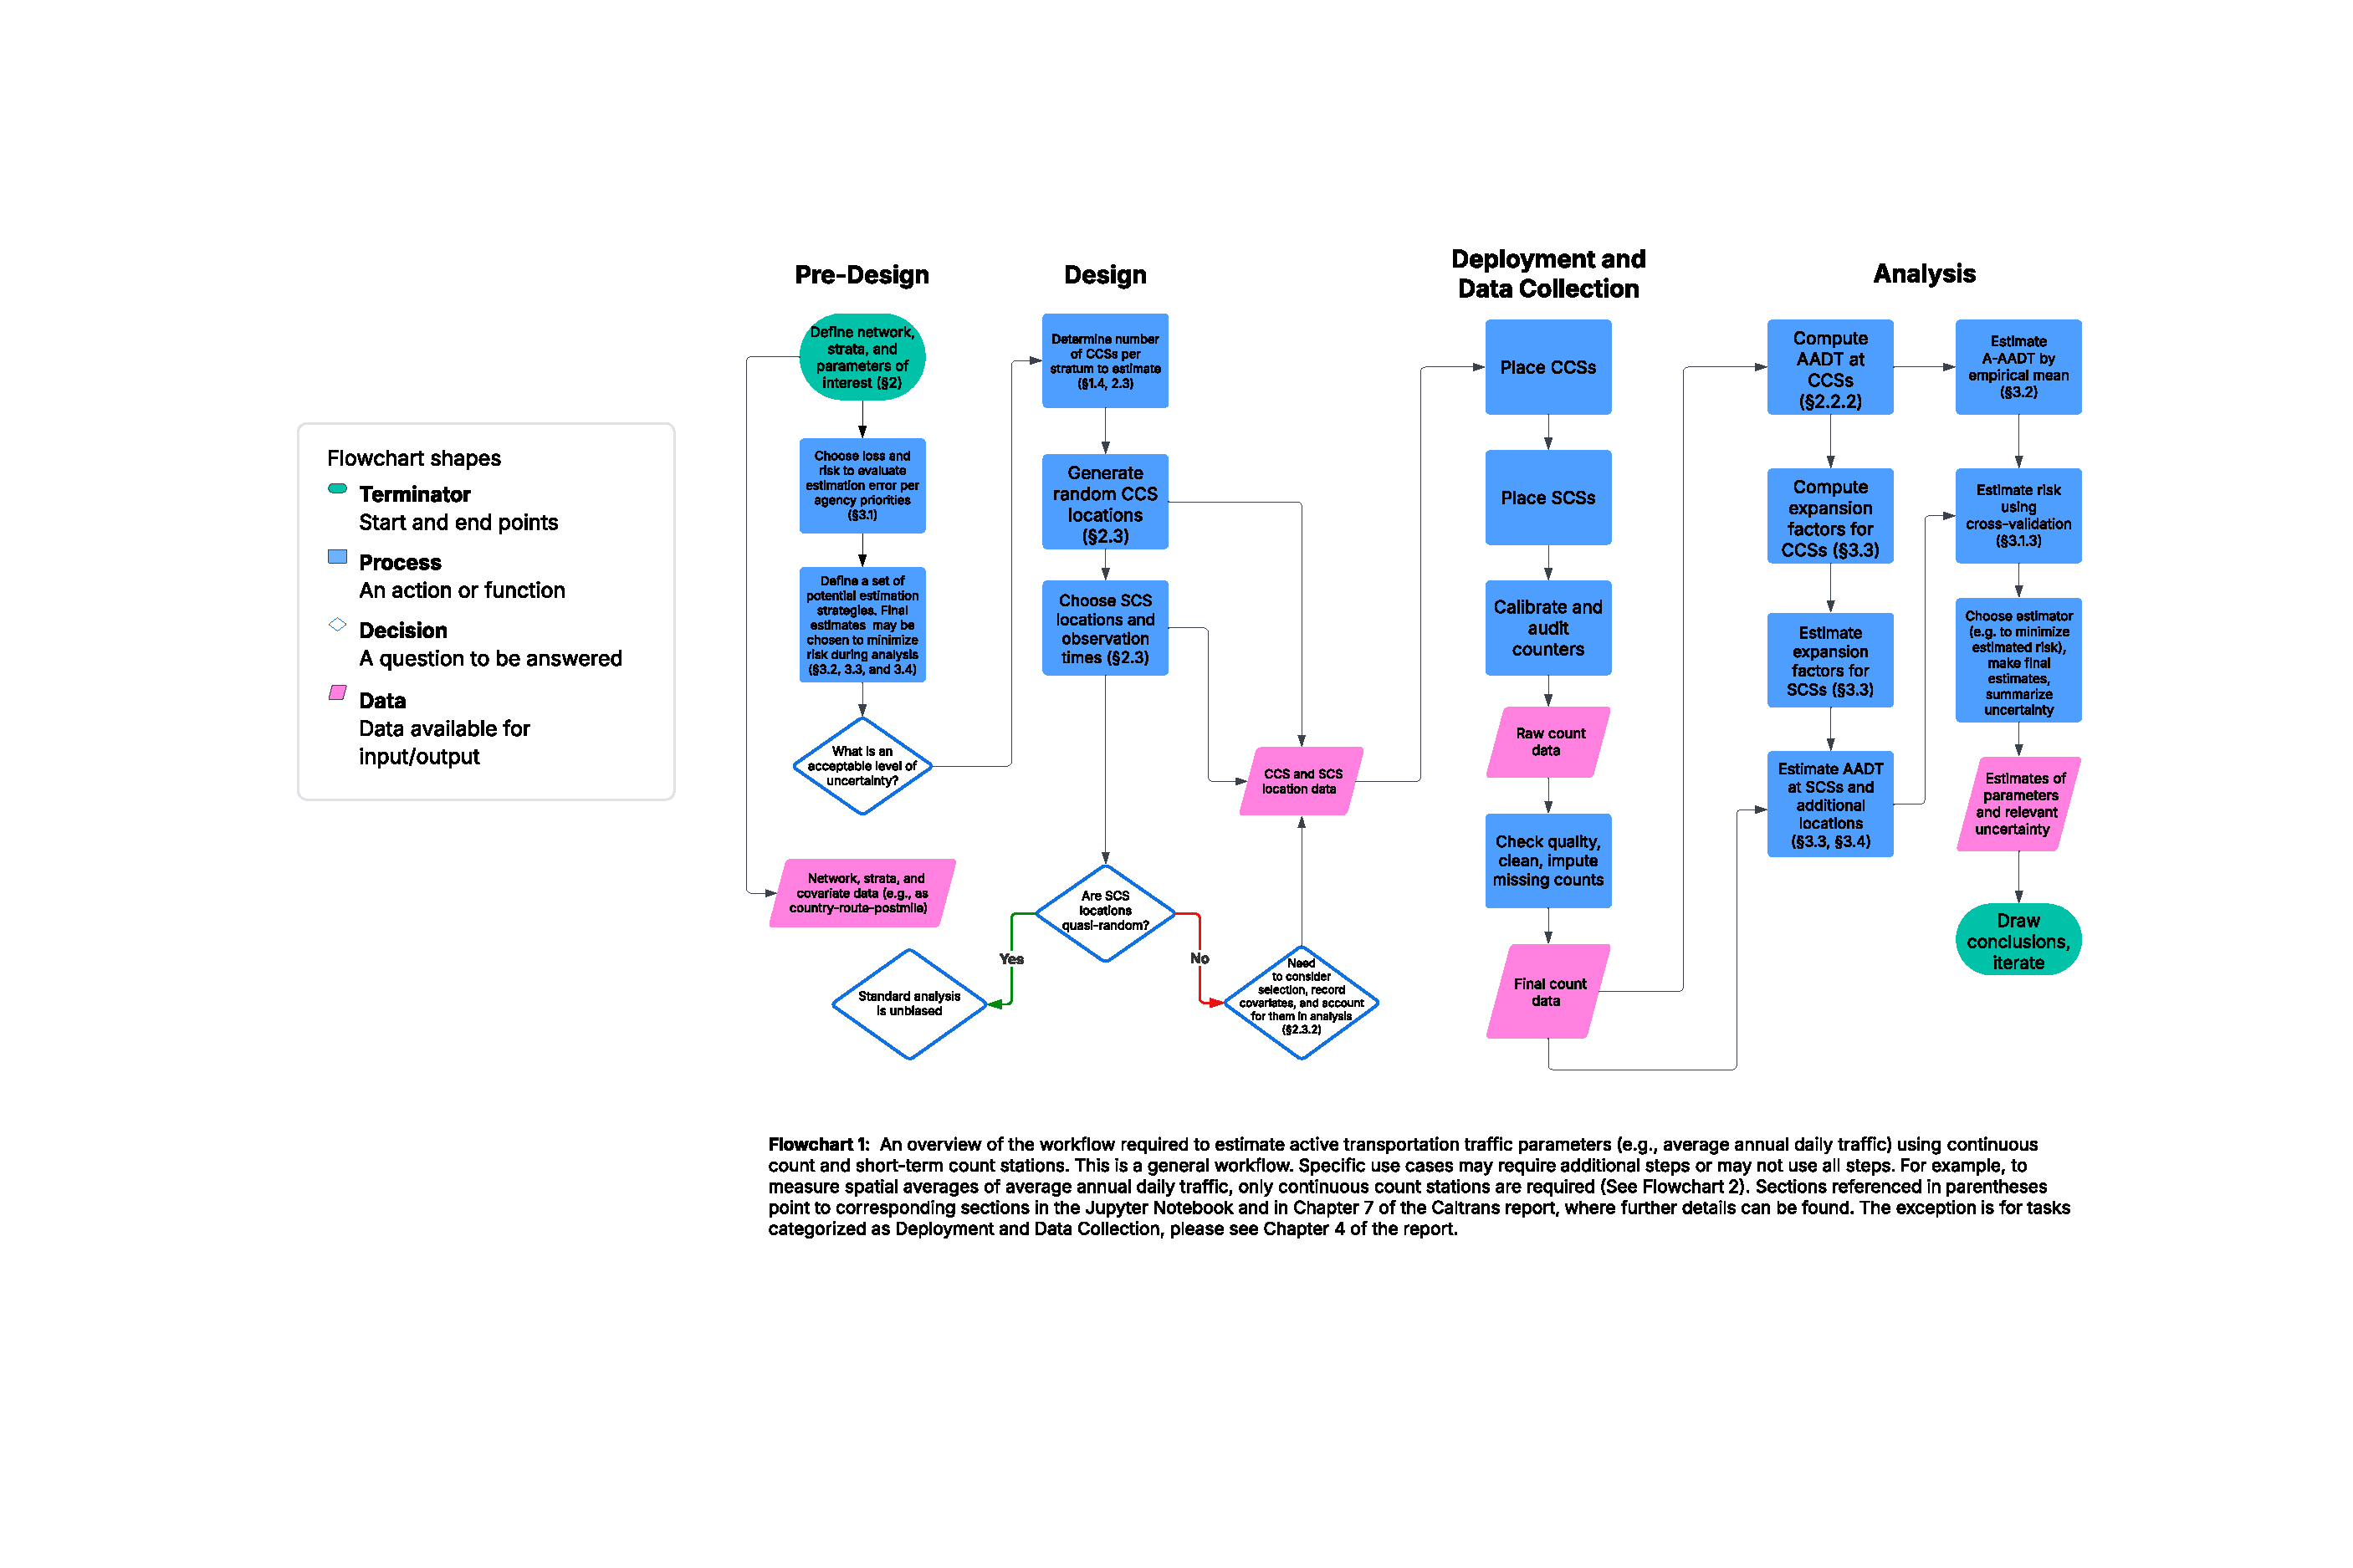
\includepdf[pages = 1]{../Output/Flowchart_overview.pdf}

    \subsection{Previous work on AADT}\label{previous-work-on-aadt}

AADT estimation is well established for motor vehicle estimates, with a
history spanning more than 100 years. In the 1920s, government agencies
recognized the need for accurate, standardized traffic estimates in
response to expanding motor vehicle ownership and infrastructure
requirements. The Federal-Aid Highway Act of 1944 tied traffic estimates
to federal funding, while the use of SCS counts in conjunction with
statistical methods became increasingly common between 1940 and and the
mid-1950s (\href{https://trid.trb.org/View/365623}{Albright, 1991}). The
1966
\href{https://onlinepubs.trb.org/Onlinepubs/hrr/1966/118/118-005.pdf}{Drusch
report} codified the factor group method as a standard AADT estimation
technique for motor vehicle traffic
(\href{https://nap.nationalacademies.org/catalog/27925/guide-on-methods-for-assigning-counts-to-adjustment-factor-groups}{NCHRP,
2024}). Factor groups remain the standard for estimating AADTs from SCS
data, as evidenced by the recommendations in the FHWA's 2018
\href{https://www.fhwa.dot.gov/policyinformation/pubs/pl18027_traffic_data_pocket_guide.pdf}{Traffic
Data Computation Method Pocket Guide} and 2024
\href{https://www.fhwa.dot.gov/policyinformation/tmguide/}{\emph{Traffic
Monitoring Guide}} (TMG). A comprehensive review of AADT estimation via
the factor group is available in
\href{https://nap.nationalacademies.org/catalog/27925/guide-on-methods-for-assigning-counts-to-adjustment-factor-groups}{NCHRP
(2024)} (pages 8-10), but that report does not dwell on the design. The
assumption that CCSs ``are equivalent to a simple random sample
selection,'' quoted from the
\href{https://www.fhwa.dot.gov/policyinformation/tmguide/}{TMG}, is not
meaningful without both (a) a well defined population and (b) either
genuinely random location selection or a reasonable argument that
locations can be treated \emph{as if} they are random---that they are
not subject to selection bias. In practice, station locations are
typically chosen for specific a priori reasons like high traffic volume
or accident rates, so selection bias is the rule rather than the
exception and CCS data are not representative of a larger population of
interest. We include an extended discussion of the design issues in CCS
and SCS placement below. In short, to estimate AADT at SCSs it suffices
if SCSs are representative of CCSs (via random partioning, for example),
but that assumption is not sufficient to estimate AADT at locations with
no station whatsoever.

Beyond the factor group method, prediction algorithms---including
ordinary least squares, generalized linear models, Kalman filters,
decision trees, random forests, boosting, nearest neighbors, and
ARIMA---have long been applied to motorized traffic estimation
(\href{https://www.sciencedirect.com/science/article/abs/pii/S1389128620311877}{Boukerche
and Wang, 2020}). These are surveyed in some detail in
\href{https://nap.nationalacademies.org/catalog/27925/guide-on-methods-for-assigning-counts-to-adjustment-factor-groups}{NCHRP
(2024)}. More recently, researchers have deployed a host of
sophisticated prediction methods often dubbed \emph{deep learning} or
\emph{artificial intelligence} and primarily based on variants of neural
networks (e.g., \href{https://arxiv.org/pdf/1707.01926}{Li et al
(2018)}, \href{https://arxiv.org/pdf/1709.04875}{Yu et al (2018)}).

Agencies have become increasingly interested in measuring and estimating
AADT for AT (in addition to motor-vehicle traffic) since the early 2000s
(\href{https://www.oregon.gov/odot/Programs/ResearchDocuments/SPR772_Bicycle_PedestrianTechnologies.pdf}{Nordback
et al, 2016}). Since 2013, the FHWA \emph{Traffic Monitoring Guide} has
included an entire chapter on AT counting technologies. The AT field has
generally borrowed methods from the motor vehicle sector, including the
factor group method for AADT estimation. Similarly, researchers have
used algorithmic regression methods for estimating AT utilization at
various points
(\href{https://www.sciencedirect.com/science/article/abs/pii/S0169204612001910}{Hankey
et al, 2012};
\href{https://www.jtlu.org/index.php/jtlu/article/view/892}{Chen et al,
2017};
\href{https://www.jtlu.org/index.php/jtlu/article/view/296}{Strauss and
Miranda-Moreno, 2013}). Recent work has attempted to map AADT for AT
using LBS data and deep learning (e.g.,
\href{https://arxiv.org/abs/2410.08522}{Gupta et al (2024)}). As
discussed above, there are systematic biases in LBS data
(\href{https://www.sciencedirect.com/science/article/pii/S0169204623000051}{Venter
et al, 2023}) and in smartphone data more generally
(\href{https://hbr.org/2013/04/the-hidden-biases-in-big-data}{Crawford,
2013}) that make generalizing from LBS data unreliable. Our goal of
estimating AADT at point locations using CCS and SCS data is more
modest, but under design assumptions the estimates are unbiased and
their uncertainty can be reliably quantified.

While translating long-used methods from the motor vehicle literature
seems straightforward, there are measurement and data sparsity issues
that are unique to AT. In particular, AT sensors can be plagued by
various sources of measurement noise
(\href{https://www.oregon.gov/odot/Programs/ResearchDocuments/SPR772_Bicycle_PedestrianTechnologies.pdf}{Nordback
et al, 2016}), and in most places in the U.S., there is far less
pedestrian and bicycle traffic than motor vehicle traffic
(\href{https://arxiv.org/abs/2410.08522}{Gupta et al, 2024}). Even a
small misclassification rate (a sensor mistaking a car for a pedestrian
or bicycle, or vice versa) can cause large errors in SCS and CCS counts
(\href{https://trec.pdx.edu/sites/default/files/smol-IBPI\%20Guide\%20to\%20Bicycle\%20\%26\%20Pedestrian\%20Count\%20Programs_final.pdf}{Nordback,
2013};
\href{https://www.oregon.gov/odot/Programs/ResearchDocuments/SPR772_Bicycle_PedestrianTechnologies.pdf}{Nordback
et al, 2016};
\href{https://www.researchgate.net/publication/377362665_DATA_CHECKS_FOR_BICYCLE_AND_PEDESTRIAN_COUNTS}{Glazer
et al 2024}).

    \subsection{Designing a network of counters to make reliable statistical
estimates of AT
traffic}\label{designing-a-network-of-counters-to-make-reliable-statistical-estimates-of-at-traffic}

It is critical to begin at the \emph{design} stage: unless data are
collected appropriately, the data cannot be used to estimate traffic
reliably anywhere it is not directly measured, i.e., anywhere there is
not a CCS. Randomization is the key to sound statistical inference. If
CCS sites are selected using a suitable random design, the resulting
data can be used to estimate average properties of traffic for all or
part of the road network, for example, for particular types of
infrastructure in particular geographic areas.

Generically, we call portions of the transportation network ``strata.''
\emph{Pre-stratification} involves selecting count sites by partitioning
the network into non-overlapping groups of locations, then selecting
locations separately from each such group. Post-stratification involves
combining samples from groups of CCSs that have common features, without
ensuring ahead of time that each such group will contain some number of
CCSs.

Pre- or post-stratification can improve the estimates for subsets of the
transportation network. ``Pre-stratification'' occurs at the design
stage, and entails placing CCSs at random locations within strata,
independently across strata. Pre-stratification guarantees that the
sample size in a subpopulation of interest (e.g., rural bike paths in
District 1) is adequate to get estimates of the required precision for
that subpopulation. It has a history of use in active transportation,
including to estimate ``bicycle miles traveled'' in the Twin Cities
region
(\href{https://www.cts.umn.edu/publications/report/sample-based-estimation-of-bicycle-miles-of-travel-bmt}{Davis
and Wicklatz, 2001}) and in Washington state
(\href{https://www.wsdot.wa.gov/research/reports/fullreports/828.1.pdf}{Nordback
and Sellinger, 2014}).

``Post-stratification'' occurs at the \emph{analysis} stage, and entails
estimating averages within strata defined by covariates that were not
used to design the sample. It allows inferences to be drawn about a
subset of the network that was not specifically targeted when the
locations of CCSs were selected, but consequently cannot guarantee that
there will be enough CCSs in that subset to estimate properties of
traffic with adequate accuracy.

In AT sampling, strata correspond to subsets of the network where AT
estimates are desired (by the agency): stratification ensures that there
are enough stations in each subset to make reliable estimates of traffic
in each of them. In contrast, the typical use of stratified sampling in
statistics is to improve population-level estimates by taking advantage
of homogeneity within subsets: the strata themselves may not be of
particular interest, but are merely a tool to enhance the estimate of a
global quantity (e.g., the total yearly traffic across the entire
population or network). Strata are not the same as factor groups, even
though both involve dividing the population up into subgroups. Factor
groups are sets of CCSs that are used to generate expansion factors,
which are then combined with an SCS counts to estimate an AADT. Factor
groups are generally constructed by post-stratification: finding sets of
CCSs with similar covariates and are thus expected to have similar
expansion factors.

We will discuss estimating two kinds of quantities: an average within a
pre- or post-stratum, and traffic at a particular location within a
stratum where no CCS was deployed. If CCS locations are selected at
random within pre-strata, the first kind of quantity can be estimated in
a way that is statistically unbiased and that has known uncertainty. To
estimate the second kind of quantity in a way that is statistically
unbiased is in general possible only if the specific location is
selected at random from the stratum, \emph{even if a SCS is installed at
that location}. Traffic at randomly selected CCSs is representative of
traffic at SCS locations if the SCS locations are also selected at
random. However, SCS locations are often selected because those
locations are interesting, not because they are typical of their stratum
or genuinely generated at random. We provide approaches whose
statistical performance is guaranteed when SCS locations are ``as if''
selected at random. Post-stratification may help to meet this
assumption, but it is ultimately up to the user to decide whether (as
if) random selection is an adequate approximation to reality.

As an example, the agency might pre-stratify on broad geography
(Caltrans District), infrastructure (road, trail, path, etc.), and
anticipated AT traffic (e.g., fewer than 10 cyclists per day, 10-100,
and 100+), selecting CCS locations at random within each stratum. Using
data from those CCS locations, the agency can measure AADT and other
summaries of traffic at those CCS locations and can make unbiased
estimates of the overall traffic or ``average'' AADT within each
stratum. The agency might also care about divisions smaller than the
original strata. To estimate traffic in those areas, the agency might
then poststratify on finer geography (City of Oakland, unincorporated
Humboldt, etc.) or other aspects (proximity to schools, proximity to
roadways, estimated motor vehicle traffic, etc) and use the average
within a poststratum to estimate ``average'' AADT within that
post-stratum; under these assumptions, such estimates are also
statistically unbiased and their uncertainty is well understood.

Furthermore, an unbiased estimate of average AADT in a pre-stratum or
post-stratum is an unbiased estimates of the same parameter for a
location \emph{selected at random} from the pre-stratum or post-stratum,
and uncertainties can be estimated from the variability of the CCS
measurements within the stratum.

However, if the location within the pre- or post-stratum is not selected
at random but because it is of special interest, any estimate derived
from the CCS data within the stratum can be biased and its uncertainty
cannot be quantified without assumptions about how much traffic can vary
between CCS locations. In this situation, it is common to augment CCS
data in the stratum with SCS data collected at the particular locations
of interest. To estimate AADT at purposively chosen sites, we make the
convenient but strained assumption that a given site is selected ``as if
at random'' from the pre-stratum or post-stratum. The statistical bias
of the resulting estimates and the accuracy of their uncertainties
depend on whether that assumption is approximately correct.

As an example, suppose an SCS is deliberately placed at a location near
a school. The expansion factors for that SCS could be estimated from (a)
all CCSs in the stratum or (b) all CCS in the stratum that are near a
school. Choice (b) may lead to an AADT estimate with lower bias and a
better sense of associated uncertainty because the SCS in question is
better represented by the subset of CCSs near schools than by all CCSs.

We recommend stratified sampling to ensure there is an adequate number
of CCSs in the main divisions of the population, e.g., rural and urban
areas, bike paths and bike lanes. ``Adequate number'' depends on the
desired precision of the estimates and on the variability of traffic
across locations within each stratum (which typically will not be known
until stations are deployed, although one might deploy SCSs to get pilot
estimates). There is no magic number, but at a \emph{minimum}, we would
recommend 30 CCSs per stratum. That might be inadequate for many
purposes, for instance, if the variability of AADT within the stratum is
large or if there will be post-stratification into finer geography at
the analysis stage. The selection of strata should be informed by
subject matter experts at the agency to ensure that it is possible to
make adequately precise estimates for the places of interest to
management. We will assume that post-stratification is a finer division
of the sampling strata: no post-stratum has any locations in common with
more than one initial stratum. It is possible to construct estimates for
post-strata that intersect multiple pre-strata, but we do not address
the mechanics of that here.

    \section{Formalizing the questions
statistically}\label{formalizing-the-questions-statistically}

As mentioned above, CCS and SCS data have errors and uncertainties:
counters need to be calibrated. The development below assumes that count
measurements are perfect, i.e., that CCS and SCS counts are the true
numbers of bicycles and/or pedestrians that passed that location while
the counters were in place.

Our exposition focuses on a single stratum or post-stratum and assumes
that the CCS locations were selected at random uniformly within that
stratum. Generally, this involves deploying new counters: previously
deployed CCS locations were typically chosen deliberately rather than
randomly. The development below explains how one would analyze data from
an as-yet-unbuilt network of CCSs designed to support statistical
inferences.

\emph{Average AADT} (A-AADT) means the spatial average of the AADT
within a stratum, uniformly weighted across all points in the stratum.
A-AADT for a given year is a fixed, unknown parameter. We will assume
that CCS locations are selected uniformly at random within a stratum,
i.e., that every location in a stratum is equally likely to receive a
CCS. We will also assume that the CCS data are complete (there is no
missing data, such as temporal gaps in measurement) and perfect (there
is no measurement error, e.g.~missed counts or added counts).

We consider three problems:

\begin{itemize}
\tightlist
\item
  Estimating A-AADT from CCS data, which can be achieved by taking the
  usual (unweighted) sample mean within the pre-stratum or post-stratum
  of interest.
\item
  Estimating AADT at a particular location in a stratum where there is
  no CCS from CCS data collected from the stratum, which might involve
  modeling how AADT varies within a stratum.
\item
  Estimating AADT at a particular location in a stratum using CCS data
  augmented with SCS data, which typically involves adjusting for
  temporal patterns and taking into account observable features of the
  target location (\emph{covariates}), for instance using the factor
  group method.
\end{itemize}

We introduce formal notation and propose a variety of estimation
strategies in what follows.

    \subsection{Statistical aside: parameters, estimators,
estimates}\label{statistical-aside-parameters-estimators-estimates}

A \emph{parameter} is a property of the population; for instance, the
true AADT at a particular location or the true A-AADT across a stratum.
Parameters do not depend on the observed data. An \emph{estimator} is a
function of the observed data that does not depend on any unknown
aspects of the population. For example, multiplying the total measured
traffic at a location for a week by 52 is an estimator of the annual
traffic at that location--although it might not be a good estimator.
When the data come from a random sample, the estimator is random and can
be described by a probability distribution (its \emph{sampling
distribution}). An \emph{estimate} is the realized value of an
estimator. For instance, if the measured traffic in the previous example
is 500 bicycles, then the estimate is 500 \(\times\) 52 = 26,000
bicycles. The verb ``calculate'' should be associated with a parameter
while ``estimate'' should be associated with an estimator.

There is some confusion in the literature about whether AADT is a
parameter or an estimate; we treat it as a parameter. Because we are
assuming that CCS data are perfectly accurate, AADT can be
\emph{calculated} wherever there is a CCS, but can only be
\emph{estimated} where there is no CCS. Finding a good estimator of AADT
from incomplete or noisy data requires appropriate statistical analysis.

    \subsection{Notation: Population, parameters, estimators, and
estimates}\label{notation-population-parameters-estimators-and-estimates}

In general, we will use bold font Roman letters (e.g., \(\mathbf{y}\))
to denote
\href{https://en.wikipedia.org/wiki/Euclidean_vector}{vectors}. For
instance if \(\mathbf{y} = [1, 2, 5]\), \(\mathbf{y}\) consists of the
numbers 1, 2, and 5, in that order. We generally use vectors to
represent multiple quantities simultaneously, e.g.~a vector may
represent the week 1 count for every CCS in the stratum or the list of
expansion factors for every time period for a particular CCS. We will
use overbars to denote averages (\(\bar{y}\), \(\bar{\bar{y}}\)), and
carets (``hats'') to denote estimators and estimates (\(\hat{y}\)). The
symbol \(r\) denotes location in space, and \(t\) denotes time. We
typically use lower-case Roman letters for constants and parameters. The
expected value and variance of a random variable \(Y\) are denoted
\(\mathbb{E} [Y]\) and \(\mathbb{V}[Y]\), respectively.

    \subsubsection{Population}\label{population}

There is some network of infrastructure--roads, paths, trails, and so
on. Each point in that network can be uniquely identified with a value
between 0 and 1. To do so, imagine laying the segments of the road
network end-to-end, with the first point on the first segment lying at 0
and the last point of the last segment lying at mile \(x\); dividing
every point by \(x\) then squashes the network to \([0,1]\) so that 0 is
the start of the network and 1 is the end. For instance, if there are
1,000 miles of infrastructure, milepost 0 of the road whose name comes
first in the alphabet could be identified with the point 0; the first
mile of that road maps to the interval \([0, 1/1000]\). If that road is
\(m\) miles long, the road maps to the interval \([0, m/1000]\). The
next road alphabetically starts at \(m/1000\), and so on. In this way,
we can think of any aspect of traffic (for instance, AADT) as a function
defined on the interval \([0, 1]\). We stress that the interval
\([0,1]\) is merely one way to \emph{represent} or \emph{embed} a
continuous road network. We could just as easily represent the road
network by the interval \([0,500]\). Alternatively, the road network
could be represented in two dimensions, e.g., by \((x,y)\) with \(x\)
the latitude and \(y\) the longitude for every point in the network.
However, compared to the standard interval \([0,1]\), these alternative
embeddings add unnecessary complexity to conceptualizing the population
of interest and to the subsequent design and analysis of count data.

The network is \emph{partitioned} into \(K\) strata in such a way that
any piece of infrastructure is in exactly one stratum. In the
development below, we consider a single stratum. We note that the
development extends immediately to a network with multiple strata by
implementing the techniques for each stratum in turn. Narrowing focus to
a single stratum simplifies our notation.

Time is discrete and indexed by \(t \in \{1,\ldots, t_{\max}\}\), where
\(t_{\max}\) is the total number of counting periods in the year of
interest. The counting period might be a 15-minute increment, an hour, a
day, or a week, for instance.

We assume we are interested in AADT for a particular historic year.
Results from one year are immediately stale unless some aspect of AADT
is approximately \emph{stationary} from year to year. For instance,
expansion factors for a particular year may continue to be useful in
future years despite the fact that traffic varies from year to year,
provided annual \emph{patterns} of traffic do not change (that they are
stationary from year to year). If patterns also change, all bets are
off. For example, compared to motor vehicle traffic, bicycle and
pedestrian traffic are particularly sensitive to seasonal, annual, and
secular variations in weather. Such variations (e.g., a cooler summer
and warmer, dryer winter) could effect traffic patterns, making
forecasts less accurate.

Let \(y_t(r)\) denote the count of traffic in the \(t\)th time interval
at location \(r\) in the stratum. Let
\(\mathbf{y}(r) = [y_t(r)]_{t=1}^{t_{\max}}\) be a length-\(T\) vector
representing all the counts at point \(r\) over the course of the year.
The counts \(\mathbf{y}(r) = [y_t(r)]_{t=1}^{t_{\max}}\) are fully
observed at locations \(r\) where there are CCSs, partially observed at
locations where there are SCSs, and not observed at all for points \(r\)
with neither a CCS nor an SCS. The population comprises \emph{all}
counts \(\mathbf{y}(r)\) for \(r \in [0, 1]\), even at locations \(r\)
with no observations. Any parameter of interest (e.g.~AADT) at any point
\(r\) could be calculated if the entire population were known. Finally,
every location in the population has a length-\(p\) vector of
\emph{covariates} \(\mathbf{x}(r) := [x_j(r)]_{j=1}^p\) recording
features of the location.

    \subsubsection{AADT at a point location}\label{aadt-at-a-point-location}

The AADT at location \(r\), is the temporal average of its count vector:
the total amount of AT traffic passing location \(r\) over the course of
the year divided by the number of days in the year. In symbols, we
define the AADT at \(r\) as \[
\bar{y}(r) := \frac{1}{365} \sum_{t=1}^{t_{\max}} y_t(r)
\] for an ordinary year (not a leap year). We stress that the counts
\(y_t(r)\) \textbf{may be partially or entirely unobserved} at location
\(r\): AADT is a parameter, not an estimate based on observed data. The
AADT for a given location in a given year is the \emph{actual} total
count of traffic passing that location in that year, divided by the
number of days in that year. It is not the count observed by an SCS or
even observed by a CCS (which may have measurement errors or gaps).
Disregarding the potential for measurement error and missing data, AADT
can simply be calculated wherever there is a CCS station, since the
entire count vector is observed, and thus the total count is known. The
collection of AADTs \(\{\bar{y}(r)\}_{r \in [0, 1]}\) for the whole
population represents the set of target parameters that the agency might
wish to know. In reality, only the AADTs at locations with CCSs are
calculable; AADT at other locations must be estimated.

    \subsubsection{A-AADT within strata}\label{a-aadt-within-strata}

The \emph{average AADT}, A-AADT, is simply the spatial average of the
AADTs over the entire stratum. That is, the A-AADT is the total A-AADT
in the stratum divided by the size of the stratum. If location were
discrete (i.e., if the stratum were represented by a finite list of
locations), the A-AADT would be a simple averageL: the sum of the AADT
at every location divided by the number of locations in the list. Since
the stratum is a continuous network with uncountably infinite locations,
the A-AADT is instead expressed in symbols as an integral over the
stratum. \[
\bar{\bar{y}} := \int_0^1 \bar{y}(r) dr.
\] A-AADT (or total traffic) may be an important parameter its own
right, e.g., if funding is dispersed to strata proportional to the
amount of traffic in each. An A-AADT estimate can also serve as a
rudimentary estimate of AADT at a given point in the stratum. This
estimation technique is discussed further below.

    \subsubsection{AASHTO-AADT}\label{aashto-aadt}

Some studies focus on a different annual average, the
\href{https://www.fhwa.dot.gov/policyinformation/tmguide/tmg_2022/Appendix-L-AASHTO-AADT-Calculation.pdf}{AASHTO-AADT},
rather than AADT as defined above. The AASHTO-AADT takes the average
traffic on each day of the week each month (e.g., the average Monday in
January), averages the 12 monthly day-of-week averages for each of the
seven days with equal weight (e.g., the average of the average Monday in
January, the average Monday in February, \ldots, and the average Monday
in December), then averages those seven averages with equal weight. This
is a different parameter because the number of Mondays varies from month
to month and year to year. If desired, AASHTO-AADT at a point location
or stratum average AASHTO-AADT could be the target parameter, in place
of AADT and A-AADT. AADT can be calculated from annual total traffic at
a site; AASHTO-AADT requires daily totals.

    \subsection{Data}\label{data}

\subsubsection{Random selection}\label{random-selection}

We assume that error-free and complete CCS counts are observed at
\(n_c\) discrete locations \(\{r_j^c\}_{j=1}^{n_c}\) selected uniformly
and independently at random from the stratum. (Deviations from this
assumption are discussed in the next section.) Every location within the
stratum has an equal probability to be sampled for selection; it is
possible, but outside the scope of this document, to sample locations
with unequal (but still known) probabilities and adjust for the unequal
weighting at the analysis stage (e.g.,
\href{https://projecteuclid.org/journals/statistical-science/volume-32/issue-2/Probability-Sampling-Designs--Principles-for-Choice-of-Design-and/10.1214/16-STS606.full}{Tille
and Wilhelm (2017)}).

We may set \(n_c\) to be small in strata that are relatively low
priority (e.g., because they are suspected to have very low traffic),
and high in strata that are higher priority. Strata with relatively high
variability in AADT should also receive more CCSs (especially when that
variability is not well proxied by covariates) when it is important to
estimate A-AADT more precisely in that stratum. For instance, consider a
``less variable stratum,'' wherein AADT is distributed uniformly between
400 and 800 (A-AADT = 600), and a ``more variable stratum,'' wherein
AADT is distributed uniformly between 100 and 1100 (A-AADT = 600). When
estimating A-AADT using CCS data, the less variable stratum would need
fewer CCSs than the more variable stratum would in order to achieve a
given level of precision.

Deploying CCSs at random locations makes it possible to quantify the
uncertainty in estimating A-AADT (conversely, without random sampling
the uncertainty cannot be quantified reliably). This model may not be
realistic for CCSs that have already been deployed. It is our
understanding that existing CCS locations in California were not
selected at random, but were usually selected because the sites were in
some sense special (for instance, because there were collisions, because
new infrastructure was contemplated or had been installed, or because
the agency wanted to measure motor vehicle traffic and decided to
measure AT traffic at the same time). It is wishful thinking to believe
that A-AADT can be estimated well from CCS data unless the CCS locations
are representative. (And it is wishful thinking to believe that AADT can
be estimated reliably from SCS data at some location using CCS data from
other locations unless the SCS site is suitably similar to the CCS
sites.)

While the locations of already-deployed CCSs were not selected at random
(the \emph{design} assumption is false for extant counters), Caltrans
can deploy stations at random within strata (code is provided below) to
create a statistical network of counters to make it possible to estimate
A-AADT reliably, with known uncertainties.

Finally, we assume that SCSs are deployed at \(n_s\) locations
\(\{r_j^s\}_{j=1}^{n_s}\) in the stratum. Unless these \(n_s\) locations
are also selected at random, they will be of little help in estimating
A-AADT for the stratum. Unless there is a stable relationship between
AADT and covariates of sites, having an SCS at location \(r\) is not
necessarily helpful in estimating AADT at the point \(r\).

    For each CCS location \(r_i^c\), \(i = 1, \ldots, n_c\), the entire
count vector \(\mathbf{y}(r_i)\) is observed.

For each SCS location \(r_i^s\), \(i = 1, \ldots, n_s\), we only observe
counts at times \(\mathbf{t}_i \subset \{1,\ldots,T\}\). We will
generally assume that observations at each SCS are contiguous. (E.g., we
do not sample January 1st and January 15th without the intervening days.
If it were practical to observe non-contiguous counts, e.g., a day in
January, a day in April, a day in July, and a day in October, higher
accuracy might be possible from the same number of counts, but the
logistics and costs are likely prohibitive.)

From counts at a location \(r\) observed at random times, one can make
an unbiased estimate of AADT at that location. If the random times are
selected independently, the uncertainty of that estimate can be
characterized. In what follows, we will not necessarily assume that the
times at which SCS measurements are made at a particular location are
selected at random.

The count vectors for all \(n_c + n_s\) sampled stations can be stacked
into a matrix \(\mathbf{Y}\), where row \(j\) is \(\mathbf{y}(r_j)\) and
CCS counts are in the first \(n_c\) rows. The observed data matrix
\(\mathbf{Y}^*\) is a censored version of the matrix \(\mathbf{Y}\),
where rows \(j \in \{n_c + 1, \ldots, n_c + n_s\}\) are missing every
element except in columns \(\mathbf{t}_j\). The covariate vectors
\(\mathbf{x}_j\) can be stacked in the same order into a matrix
\(\mathbf{X}\), and the observed data can be written:
\((\mathbf{Y}^*, \mathbf{X})\).

\subsubsection{Data without random
selection}\label{data-without-random-selection}

What if station locations are \emph{not} chosen by a random selection
mechanism like the one above? For instance, a site might be selected
because it is known to have high traffic or to be particularly
dangerous. In that case, the random sampling mechanism described above
may not be a good model for the real selection mechanism generating the
data, and there is likely to be substantial bias from the selection.

For example, if CCSs are installed where yearly counts are suspected to
be high, simple extrapolation to other locations will have an upward
bias: estimates of AADT and A-AADT will tend to be too big. In some
circumstances, that bias can be modeled well enough to adjust for it
using covariates. In particular, post-stratifying on variables that
influence selection can reduce selection bias.

However, it is generally not possible to estimate selection bias from
the data alone. Contextual reasoning and experience are required to
determine if the data are sufficiently accurate to inform policy
decisions. In what follows, we propose using cross-validation to measure
the quality of predictions of long-term counts, but
\textbf{cross-validation only provides accurate quantification of
prediction risk under the random sampling assumptions}. Researchers and
policy advisors need to judge whether their data is sufficiently
representative.

Valid conclusions may still be possible in the presence of unknown
selection bias, though the scope of those conclusions may be limited. In
particular, suppose both CCSs and SCSs are a weighted (i.e., biased)
sample from a stratum and the weights are unknown, but identical for
both groups of stations: both samples are subject to the same selection
bias. For example, this occurs if SCSs and CCSs are both placed
preferentially along high traffic paths, and the (hypothetical)
probabilities of placement at a particular location can be assumed equal
for a given SCS and CCS. Then the choice of whether a given station is a
CCS or SCS is essentially arbitrary, the CCSs are representative of the
SCSs, and the A-AADT for the \(n_s\) SCSs (but not the whole stratum!)
can be estimated from observed data on SCSs and CCSs. Combined, the SCSs
and CCSs are not necessarily representative of the stratum, and it is
not possible to provide statistical guarantees about the accuracy of
stratum-level A-AADT or about AADT at locations without stations.

Even these assumptions may be unrealistic considering the historic
placement of count stations. Different counting technologies are often
used for CCSs (infrared or inductive loops) compared to SCSs (video
counts), and the technologies tend to function differently in different
settings: loops work well on trails, while video counts are better for
roads with bike lanes. Thus, in practice, SCSs may be preferentially
placed on bike lanes while CCSs are placed on trails, so that CCS counts
are not properly representative of SCS counts.

    \section{Estimation}\label{estimation}

A-AADT across a stratum and AADT at a point without a CCS can be
estimated using data from a well-designed network of count stations. We
will focus on estimation techniques that use \emph{post-stratification},
which includes the factor group method for expanding SCS counts.

An estimate of A-AADT is denoted \(\hat{\bar{\bar{y}}}\), while an
estimate of the AADT for a location \(r_i\) is denoted
\(\hat{\bar{y}}(r_i)\). If \(n_0\) estimates are made, the vector of
estimates is
\(\hat{\bar{\mathbf{y}}} := [\hat{\bar{y}}(r_j)]_{j = 1}^{n_0}\) (bold
font) while the vector of true, unknown AADTs is
\(\bar{\mathbf{y}} := [\bar{y}(r_j)]_{j = 1}^{n_0}\) (also bold font).
Roughly speaking, an estimator of A-AADT is ``good'' if the predictions
\(\hat{\bar{\mathbf{y}}}\) are close to the true AADTs
\(\bar{\mathbf{y}}\) in a sense that reflects the priorities of the
agency. Because there are countless estimators one could use, we suggest
selecting an estimator by first choosing an error measure aligned with
agency goals, then choosing an estimator that approximately minimizes
that error. Additional qualitative properties such as interpretability,
covariate sparsity, or privacy may also weigh into the choice of
estimator.

In this section, we discuss a few possibilities for defining the
distance between estimates and parameters, propose a general method to
measure that distance under random sampling assumptions using only the
observed data, and suggest some estimators of AADT and A-AADT.

\subsection{Figures of merit (loss and
risk)}\label{figures-of-merit-loss-and-risk}

\subsubsection{Loss functions}\label{loss-functions}

We denote a generic \emph{loss function} by \(\ell\). We will use the
same notation for the loss function for AADT at a point \(r_i\) and for
A-AADT. For instance, \(\ell(\bar{y}(r_i), \hat{\bar{y}}(r_i))\) is the
loss in estimating AADT at location \(r_i\), i.e., the ``cost'' incurred
by claiming that the truth is \(\hat{\bar{y}}_i\) when it is really
\(\bar{y}_i\); \(\ell(\bar{\bar{y}}, \hat{\bar{\bar{y}}})\) is the loss
in estimating A-AADT, i.e., the ``cost'' incurred by claiming that the
truth is \(\hat{\bar{\bar{y}}}\) when it is really \(\bar{\bar{y}}\).

The choice of loss function encodes priorities of the agency. In
particular, consider the following two loss functions.

\begin{itemize}
\item
  \textbf{Squared-error loss} penalizes estimates based on their squared
  distance from the true AADTs. It takes the difference between the true
  AADT and the estimated AADT and squares it (so that the loss is always
  positive). In symbols:
  \[\ell_s(\bar{y}(r_i), \hat{\bar{y}}(r_i)) := (\bar{y}(r_i) - \hat{\bar{y}}(r_i))^2.\]
  For example, if the true AADT is 30 and the estimated AADT is 33, the
  squared-error loss is \((30 - 33)^2 = (-3)^2 = 9\). Larger errors are
  penalized more (an error of \(2 \epsilon\) incurs 4 times the loss as
  error \(\epsilon\)), and there is no adjustment for the size of
  stations: an off-by-5 error in an AADT estimate receives the same
  penalty whether the true AADT for station \(i\) is 10 bikes or 1,000
  bikes.
\item
  \textbf{Proportional loss} normalizes by the true counts, so the error
  is in terms of the proportion rather than volume. It takes the
  absolute value (so that the loss is always positive) of the difference
  between the true AADT and estimated AADT and divides by the true AADT
  (so that the difference is expressed in proportion to the truth). In
  symbols:
  \[\ell_p(\bar{y}(r_i), \hat{\bar{y}}(r_i)) := \frac{|\bar{y}(r_i) - \hat{\bar{y}}(r_i)|}{\bar{y}(r_i)}.\]
  Multiplying the proportinal loss by 100 gives the loss on a percent
  scale. For example, if the true AADT is 30 and the estimated AADT is
  33, the proportional loss is \(|30 - 33|/30 = 0.10\), or, multiplying
  by 100, it is \(10\%\). Proportional loss is less analytically
  tractable than squared-error loss, but prediction methods can be
  evaluated numerically for their proportional loss.
\end{itemize}

These loss functions correspond to different priorities. The choice
between them is substantive, not statistical. For squared-error loss,
the overall numerical error in counts is important, so predictions will
be particularly attuned to high-traffic stations in urban areas. For
proportional loss, percent error in counts is important, so predictions
will be more uniformly accurate across stations with varying traffic
volume. Thus, proportional loss leads to predictive equity across
stations rather than individual riders. Furthermore, proportional loss
is sensitive to errors on the order of magnitude (e.g., overestimating
the AADT by a factor of 10), not on an absolute scale (e.g.,
overestimating by 10). Agencies may prefer estimates to be ``in the
ballpark'' on most stations rather than absolutely accurate for large
stations.

Both proportional and squared-error loss are symmetric: they penalize
undershooting and overshooting by exactly the same amount. In some
situations, it might be better to use an asymmetric loss. For instance,
when the AADT estimates are inputs to models prioritizing safety
upgrades, overestimating the AADT may cost some additional money in
upgrades, while underestimating the AADT might contribute to additional
accidents and even fatalities: traffic is higher in reality than the
agency believes.

\href{https://nap.nationalacademies.org/catalog/27925/guide-on-methods-for-assigning-counts-to-adjustment-factor-groups}{NCHRP
(2024)} proposes a few performance metrics, including homogeneity of the
factors, proportional loss (``absolute percent error''), the algebraic
(signed) difference \(\hat{\bar{y}}(r_i) - \bar{y}(r_i)\), and the
coefficient of variation
\(100 \times (2 \times |\hat{\bar{y}}(r_i) - \bar{y}(r_i)|) / \sqrt{2} (\hat{\bar{y}}(r_i) + \bar{y}(r_i))\).
Homogeneity of the factors is related to squared-error loss under random
sampling assumptions, but is not itself a loss function: all else equal,
if the expansion factors for a given factor group are more homogenous,
the estimate of A-AADT within that factor group is more precise and the
squared-error loss is lower. The signed difference is not an appropriate
loss function in our view because it can be negative, and thus will not
aggregate into a sensible risk measure---overshooting an estimate for
one sample can be offset by undershooting for another sample so that the
expected loss is 0 even though no single estimate is particularly close
to the true AADT. The coefficient of variation is valid but not
particularly easy to interpret; it is equal to
\(100 \times \sqrt{2} \approx 10.4\) whenever
\(\hat{\bar{y}}(r_i) = 0\), \(0\) when
\(\hat{\bar{y}}(r_i) = \bar{y}(r_i)\), and converges back to \(140\) as
\(\hat{\bar{y}}(r_i)\) gets large.

\subsubsection{Risk}\label{risk}

Because estimates are random under the random sampling assumptions
above, the loss is a random variable. To compare estimators, we evaluate
their \emph{risk}: their expected loss under the random sampling design.
That is, for estimating AADT at location \(r_i\) the risk is
\(R(\bar{y}(r_i), \hat{\bar{y}}(r_i)) := \mathbb{E}[\ell(\bar{y}(r_i), \hat{\bar{y}}(r_i)]\)
and for estimating A-AADT the risk is
\(R(\bar{\bar{y}}, \hat{\bar{\bar{y}}}) := \mathbb{E}[\ell(\bar{\bar{y}}, \hat{\bar{\bar{y}}})],\)
where both expectations are with respect to the (deliberate) randomness
in selecting where to install CCSs. We might also evaluate the risk in
estimating AADT at \(n_0\) locations \(\{r_i\}_{i=1}^{n_0}\) as a
weighted average of the risks for the individual locations:
\[R(\bar{\mathbf{y}}, \hat{\bar{\mathbf{y}}}) := \sum_{i=1}^{n_0} q_i R(\bar{y}(r_i), \hat{\bar{y}}(r_i)).\]
The weights \(q_i := q(r_i)\) must be nonnegative and sum to 1. They
encode the priority assigned to location \(r_i\): if location \(r_i\) is
higher priority, \(q_i > 1/n_0\), and \(q_i = 1\) implies that only the
prediction accuracy at \(r_i\) matters to the agency; vice versa,
weights \(q_i < 1/n_0\) correspond to lower priority locations and
\(q_i = 0\) implies location \(r_i\) does not matter at all. If all
\(n_0\) estimation locations are prioritizied equally, the weights are
\(q_i = 1/n_0\) and the aggregate risk is the standard average of the
risks at individual locations.

\subsubsection{Estimating Risk Using
Cross-validation}\label{estimating-risk-using-cross-validation}

In practice, the risk is unknown because the true parameters (AADT or
A-AADT) are unknown. The risk must itself be estimated by a quantity
\(\hat{R}\), which is computed using only observed CCS data. This
estimate is reasonable under the random sampling assumptions described
above, because then the CCSs are representative of the entire stratum.
(If stations are not sited randomly, estimates of risk based on CCS data
may have large bias.) Furthermore, when estimating the risk of an AADT
estimate at the point \(r_i\), we are tacitly assuming that the location
\(r_i\) was itself randomly selected by the mechanism that was used to
select the CCS locations. This assumption is \emph{never} true in
practice because locations for estimation will be chosen deliberately by
the agency. If this assumption is very far from true, the estimates are
useless. There is no way to make this appraisal entirely algorithmic. It
requires specific knowledge about the network: is the location \(r_i\)
where an estimate is desired exceptional or similar to the CCSs in its
stratum, especially with regard to characteristics that are not
represented by its covariates? On the other hand, the risk of A-AADT
estimation can be quantified with no additional assumptions.

In either case, we will generally choose an estimator that minimizes the
estimated risk \(\hat{R}\), but other considerations like transparency
and interpretability may weigh in as well. For instance, when choosing
between a black-box machine learning algorithm and a simple estimator
based on taking averages over strata, we may favor the simple estimator
even if it has a higher value of \(\hat{R}\).

Now, the cross-validation risk estimate \(\hat{R}\) is an unbiased
empirical estimate of \(R\) under the random sampling assumptions
presented above. Cross-validation splits the CCS data at random into
\(K\) groups, ``trains'' the estimator on \((K-1)\) of the groups, and
evaluates the performance of that estimator on the remaining group. The
process is repeated \(K\) times, with each group held out in turn, and
the performance averaged to form the estimate \(\hat{R}\). Example code
is provided below.

Cross validation is not the only sensible choice to obtain \(\hat{R}\),
for instance, one could instead estimate \(R\) using the bootstrap or
other resampling methods. See, e.g.,
\href{https://www.statlearning.com/}{James et al.~(2023)}.

    \subsection{Estimating A-AADT}\label{estimating-a-aadt}

Estimating the A-AADT \(\bar{\bar{y}}\) across a stratum is the simplest
of the three estimation tasks we discuss, and can be done with the
smallest uncertainty. Indeed, the usual sample mean of the AADTs for the
observed CCSs (dividing the sum of CCS AADTs by the number of CCSs)
\[\frac{1}{n_c} \sum_{i=1}^{n_c} \bar{y}(r_i^c)\] is an unbiased
estimate of the true A-AADT, and has a standard error equal to the
heterogeneity (standard deviation) \(\sigma\) of AADT across the stratum
divided by the sample size \(\sqrt{n_c}\). Its risk under any loss
function of interest can be estimated using cross-validation or other
resampling methods.

CCS data could also be augmented with data from randomly located SCSs to
improve A-AADT estimates. AADT is first estimated at SCS locations using
a method like factor group estimation, described below. The AADT
estimates at SCS locations and the AADT calculations at CCS locations
are then averaged across the stratum. However, in the (hypothetical)
case that CCSs are randomly located while SCSs are purposively located,
factoring SCSs into the estimates could make them worse than the sample
mean of AADT across CCSs. Even if SCSs were randomly located, the usual
standard error estimate (ignoring the variability in AADT estimates at
the SCS sites) would underestimate the true uncertainty. The correct
formula includes the uncertainty in estimating AADT at each SCS
\[\mbox{SE}[\hat{\bar{\bar{y}}}] := \sqrt{\frac{1}{(n_c + n_s)^2}\bigg [n_c \sigma + \sum_{i=1}^{n_s} \mathbb{V}[\hat{\bar{y}}(r_i^s)] \bigg ]},\]
where the variance \(\mathbb{V}[\hat{\bar{y}}(r_i^s)] \geq \sigma\) in
each SCS AADT estimate is a function of the random sampling (hence it is
lower bounded by the heterogeneity \(\sigma\)) as well as specifics of
the station's characteristics and the estimation procedure used. If the
AADT estimate is perfect and incurs no additional error, then
\(\mathbb{V}[\hat{\bar{y}}(r_i^s)] = \sigma\) and
\(\mbox{SE}[\hat{\bar{\bar{y}}}] = \frac{\sigma}{\sqrt{n_c + n_s}}\),
which is a lower bound on the standard error of the sample mean estimate
of A-AADT when combining CCSs and SCSs.

When covariates are available, they might be used to refine estimates of
A-AADT. In essence, these methods work by estimating AADT at every point
in the stratum before averaging those estimates to estimate A-AADT.
Post-stratification may be used in this way: averages are computed
within post-strata and combined by a weighted average across post-strata
(the weights are proportional to the relative size of each post-stratum)
to estimate A-AADT. This ``adjusts'' for small, random deviations in the
representativeness of CCSs. A complete treatment of such strategies is
outside the scope of this document (but see, e.g.,
\href{https://link.springer.com/book/9780387406206?utm_medium=referral&utm_source=google_books&utm_campaign=3_pier05_buy_print&utm_content=en_08082017}{Sarndal
et al (1992)}).


The workflow for estimating A-AADT using CCS stations is illustrated by the flowchart on the next page. 
We emphasize that it is merely an example and the specific details we have chosen for illustration should not be taken as recommendations.

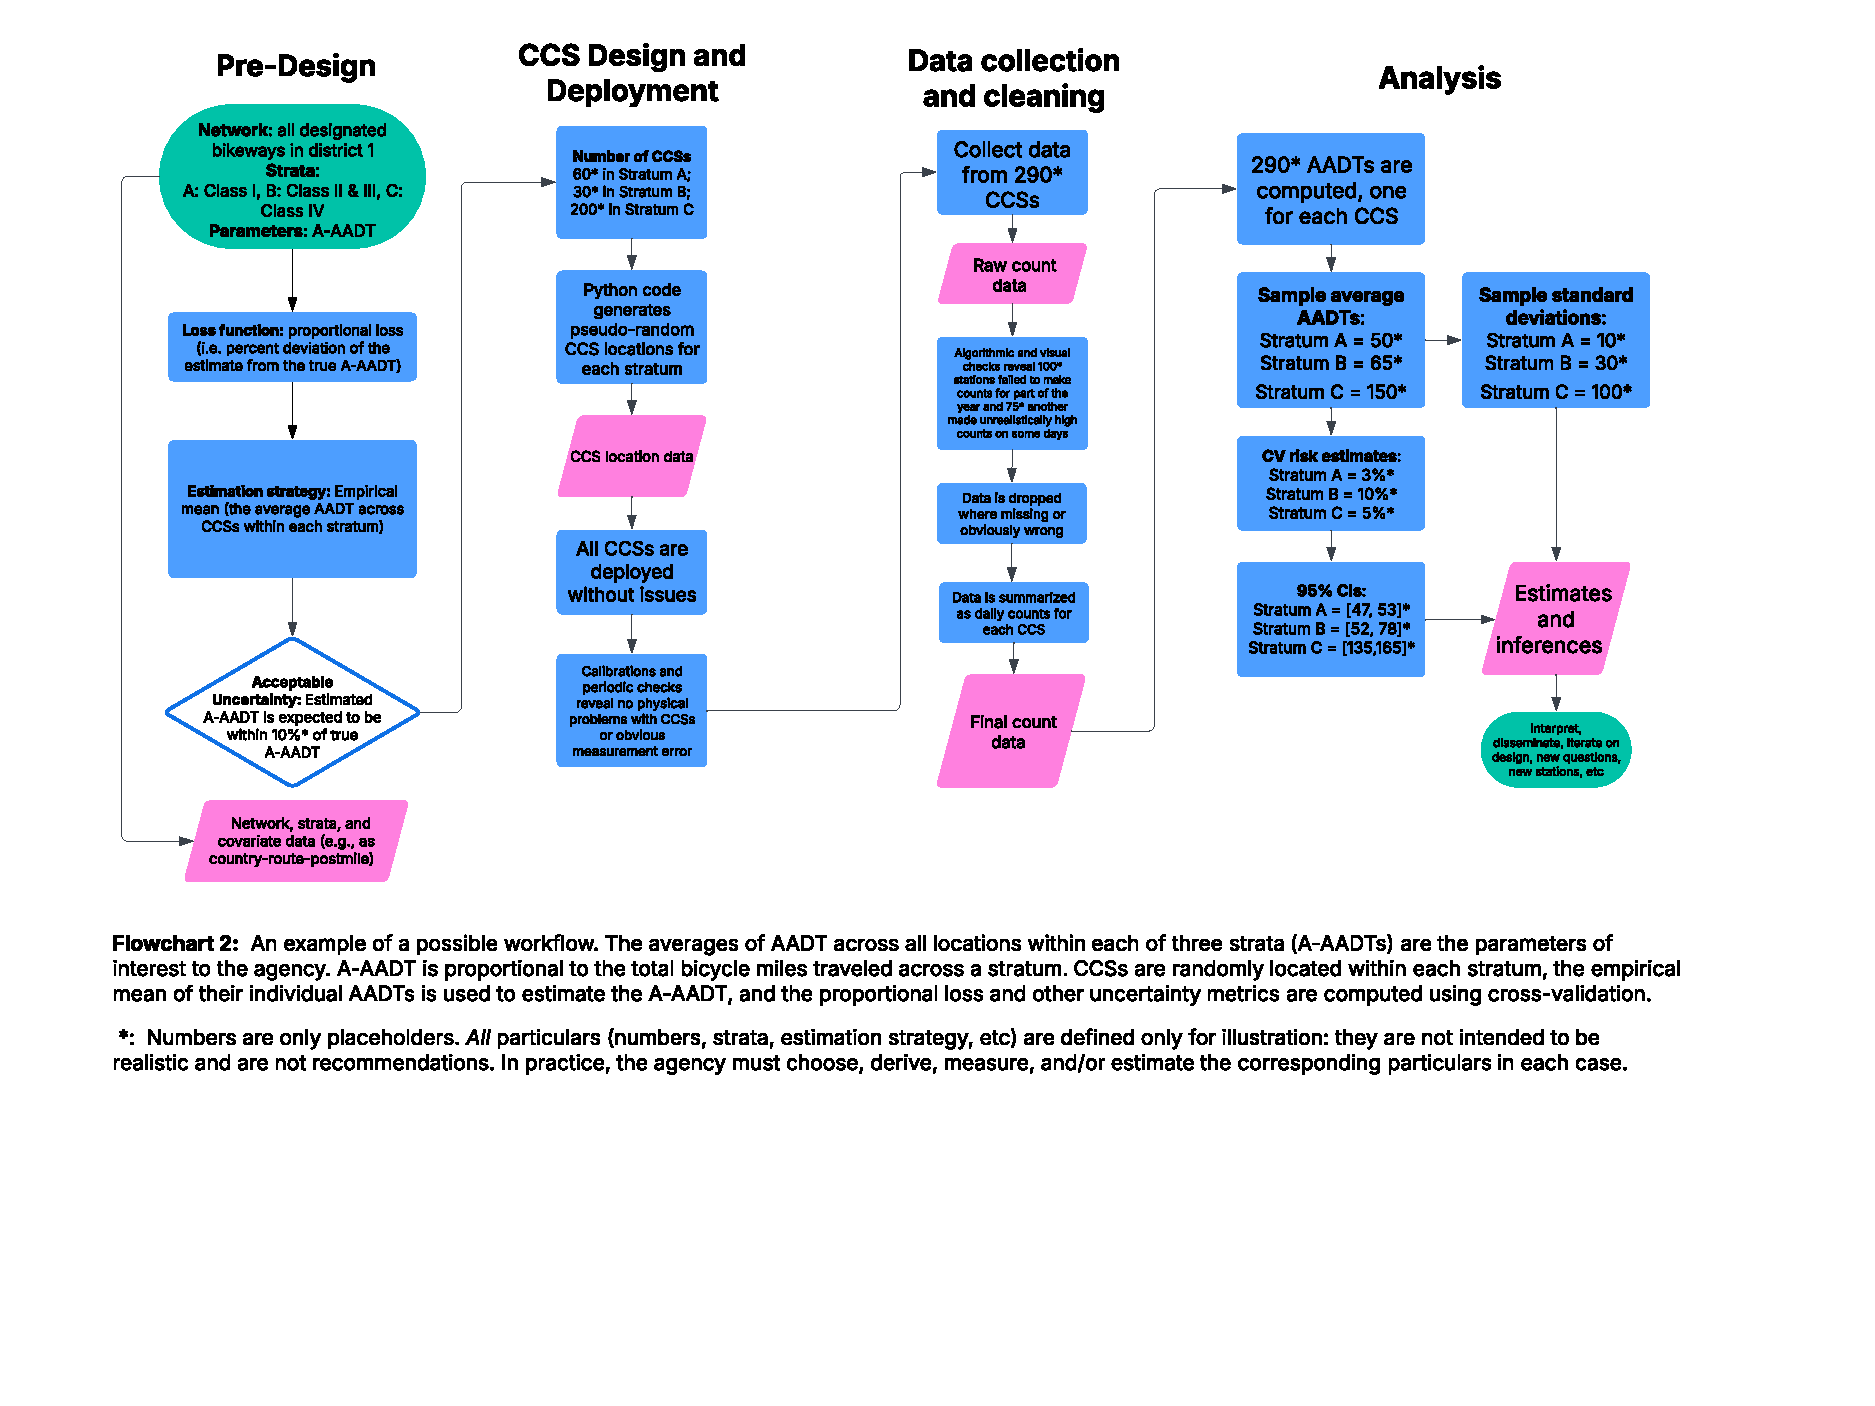
\includepdf[pages = 1]{../Output/Flowchart_example_1.pdf}

    \subsection{Estimating AADT at an SCS station using expansion
factors}\label{estimating-aadt-at-an-scs-station-using-expansion-factors}

Agencies have typically estimated motor vehicle and AT AADT at SCSs
using \emph{expansion factors}. Expansion factor methods multiply an SCS
count by a constant estimated from CCS data (the expansion factor) in
order to estimate AADT at that SCS location. The expansion factor for a
particular SCS location for a particular SCS measurement period (e.g.,
the 21st week of the year) is derived by averaging the corresponding
ratio for some subset of the CCSs. The subsets are called \emph{factor
groups}. A factor group could represent all the CCSs in the stratum or
all the CCSs within a smaller poststratum defined by additional
covariates.

Formally, a factor group for the SCS \(i\) located at \(r_i^s\) is any
subset of the CCS locations
\(\mathcal{F}_i \subset \{r^c_i\}_{i=1}^{n_c}\). Factor groups could be
based on covariates, counts, priorities, hunches, or other discretionary
considerations of the agency. The factor group average AADT is the sum
of the CCS AADTs within the factor group divided by the number of CCSs
in the factor group. Letting \(|\mathcal{F}_i|\) denote the number of
CCSs in \(\mathcal{F}_i\), this is denoted in symbols by
\[\bar{y}_{\mathcal{F}_i} := \frac{1}{|\mathcal{F}_i|} \sum_{r_j^c \in \mathcal{F}_i} \bar{y}(r_j^c),\]
and is a known and calculable quantity because the AADTs at all the CCSs
are known.

From here on, we assume that the sampling period provides a single
observed count (e.g., total traffic in a week) so that the observation
period is a scalar (\(\mathbf{t}_i = t_i\)) and the observed count can
be written \([y_t(r_i^s)]_{t \in \mathbf{t}_i} = y_{t_i}(r_i^s)\). This
assumpion accomodates daily or hourly counts that are summarized as
weekly counts; finer (e.g.~hourly) counting periods may still be used to
compute covariates, e.g., the ratio of weekend to weekday traffic, which
may be useful in defining factor groups.

For each location \(r\), there are \(T\) expansion factors
\(\{w_t(r)\}_{t=1}^T\) that would scale the observed count for each
period to the true AADT at that location. In other words, an expansion
factor at location \(r\) for period \(t\) is the AADT at \(r\) divided
by the count in period \(t\). In symbols,
\[w_t(r) := \frac{\bar{y}(r)}{y_t(r)}.\] For instance, for weekly
counts, there are 52 expansion factors for each location, one for each
week of the year. If the AADT at \(r\) is 100 and its count for week 1
is 5, the corresponding expansion factor is \(w_1(r) = 100/5 = 20\),
indicating that the AADT is 20 times higher than the week 1 traffic
(this seems reasonable since bicycle traffic may be much lower in
mid-winter compared to typical traffic for the year).

We emphasize that, in our framing, expansion factors are fixed, but
typically unknown. In fact, expansion factors are only known when there
is a CCS at \(r = r_i^c\). In that case, the expansion factors at
\(r_i^c\) can be calculated exactly (barring measurement error or
missing data) because all the counts are known. Expansion factors (fixed
parameters) may be conflated with estimates of expansion factors
(uncertain functions of observed data). As above, we attempt to
distinguish parameters from estimates of those parameters as much as
possible.

At an SCS location \(r_i^s\), the true expansion factor for the observed
period \({w}_{t_i}(r_i^s)\) is unknown (because the AADT is unknown).
Instead, we use an uncertain but known \emph{estimated expansion factor}
\(\hat{w}_{t_i}(r_i^s)\) to estimate the AADT \(r_i\). In particular,
the AADT estimate at \(r_i^s\) is estimated as the product of the
observed count at \(r_i^s\) in period \(t_i\) and the estimated
expansion factor for \(r_i^s\). In symbols,
\[\hat{\bar{y}}(r_i^s) := \hat{w}_{t_i}(r_i^s) \times y_{t_i}(r_i^s).\]
We next discuss how to obtain the estimated expansion factor
\(\hat{w}_{t_i}(r_i^s)\).

    \subsubsection{Estimating expansion
factors}\label{estimating-expansion-factors}

Expansion factors for an SCS in a particular factor group are estimated
by the average of the known CCS expansion factors across the factor
group, i.e., by the sum of CCS expansion factors across the factor group
divided by the number of CCSs in the factor group. In symbols, the
estimated expansion factor is written
\[\hat{w}_{t}(r_i^s) := \frac{1}{|\mathcal{F}_i|} \sum_{r_j^c \in \mathcal{F}_i} w_{t}(r_j^c),\]
where \(w_{t}(r_j^c) = y_{t}(r_j^c) / \bar{y}(r_j^c)\) is the known
expansion factor for the CCS station at \(r_j^c\). Each CCS expansion
factor is self-normalized by the volume of the CCS station, so the CCS
stations in factor group \(\mathcal{F}_i\) are given equal weight in
determining the overall expansion factor estimate for SCS \(i\). We call
this the ``averaging'' estimator for expansion factors.

It isn't clear whether giving equal weight to all CCSs in
\(\mathcal{F}_i\), preferentially weighting by volume, or any other form
of weighting (e.g., giving higher weight to CCSs in \(\mathcal{F}_i\)
that are closer in covariate space to SCS \(i\)) minimizes the error in
AADT estimates and hence the risk of the estimator. Under the
assumptions made above, cross-validation provides a principled way to
choose an estimated expansion factor as well as a factor grouping method
by providing an unbiased estimate of the risk under any proposed
strategy.

    \paragraph{\texorpdfstring{A factor group \(\mathcal{F}_i\) comprising
all CCSs in the
stratum}{A factor group \textbackslash mathcal\{F\}\_i comprising all CCSs in the stratum}}\label{a-factor-group-mathcalf_i-comprising-all-ccss-in-the-stratum}

The choice \(\mathcal{F}_i := \{r_j^c\}_{j=1}^{n_c}\) uses all the CCSs
in the stratum to compute expansion factors. For example, suppose we
observe 100 bikes at SCS \(i\) in week 1 (January 1-7), so that
\(y_1(r_i^s) = 100\). Also suppose there are 3 CCSs in the stratum (this
is very few) with week 1 expansion factors \(w_1(r_1^c) = 5\),
\(w_1(r_2^c) = 5\), and \(w_1(r_3^c) = 20\). That is, for CCSs 1 and 2,
the week 1 count is 5 times less than the AADT at those stations, while
for station 3 the week 1 count is 20 times less than the AADT at that
station. Since the factor group for SCS \(i\) consists of all 3 CCSs in
the stratum, we estimate the expansion factor for SCS \(i\) as
\(\hat{w}_{t}(r_i^s) = (5 + 5 + 20) / 3 = 10\). We then take the
estimate of AADT at SCS \(i\) to be its estimated expansion factor for
week 1 multiplied by its observed count for week 1:
\[\hat{\bar{y}}(r_i^s) = 10 \times 100 = 1000.\]

    \paragraph{\texorpdfstring{Refinements of
\(\mathcal{F}_i\)}{Refinements of \textbackslash mathcal\{F\}\_i}}\label{refinements-of-mathcalf_i}

Factor groups may be defined using covariates available at SCSs, or by
any other means at the discretion of the agency. Compared to using all
CCSs, refinements can improve estimates of \(\bar{y}(r_i^s)\) by giving
greater weight to CCSs that are more similar to SCS \(i\). However,
smaller factor groups do not always mean better AADT estimates: as a
rule of thumb, good factor groups are both relatively homogenous in
terms of expansion factors (the CCSs are similar to each other) and
large (there are many CCSs).

For example, suppose the pre-strata were defined as Caltrans Districts
and SCS \(r_i^s\) is located in a small rural town in District 4 (the
greater Bay Area). Rather than all CCSs in District 4, we may want to
set \(\mathcal{F}_i\) to include only CCSs in small rural towns in
District 4. This is an example of post-stratification, where the
post-strata could be derived from categorizing and combining continuous
covariates like ``population'' or ``distance from a major metropolitan
center.''

There are two main reasons post-stratification can improve estimates of
\(\bar{y}(r_i^s)\):

\begin{enumerate}
\def\labelenumi{\arabic{enumi}.}
\item
  The SCS location may not have been chosen at random. For example, it
  may have been deliberately placed in an area with a high population or
  where traffic fatalities are suspected to be high. In that case, the
  expansion factors for the whole set of (randomly located) CCSs would
  not be representative of the unobserved expansion factors at the SCS.
  The unknown expansion factors might be better estimated by refining to
  CCSs with a high population, high traffic fatalities, or similarities
  along other features that entered into the SCS location selection
  process. In short, incorporating covariate information to refine the
  factor group could help \emph{decrease bias}.
\item
  The counts can be well-approximated by a simple function of the
  covariates. For example, suppose station \(i\) is placed in a rural
  location. A working \emph{model} for \(\bar{y}(r_i^s)\) might posit
  that the AADT at \(r_i^s\) can be decomposed into the A-AADT, plus a
  deviation term for rural locations, plus an idiosyncratic (residual)
  deviation of that particular station from the average. In symbols, we
  would write
  \[\bar{y}(r_i^s) = \bar{\bar{y}} + \delta_{\mbox{rur}} \cdot 1\{r_i^s \mbox{ is rural}\} + \varepsilon(r_i^s),\]
  where \(\bar{\bar{y}}\) is the A-AADT, \(\delta_{\mbox{rur}}\) is the
  average deviation from the A-AADT for rural stations, and
  \(\varepsilon(r_i^s)\) is any residual deviation of the AADT at
  \(r_i^s\) from the average AADT of rural stations in the stratum.
  Comparing station \(i\) to other rural locations can yield a sharper
  estimate of the \(\bar{y}_i\) when \(\delta_{\mbox{r}}\) is relatively
  large, i.e., when urban/rural status is a strong predictor of average
  counts. (Correlation is enough: it is not necessary that a given
  covariate actively determine or influence the counts for this benefit
  to apply.) Thus, covariates can \emph{increase precision}.
\end{enumerate}

Both decreasing bias and increasing precision will tend to decrease
\(R\), the risk of the estimator, improving estimates in expectation. As
a rule of thumb, good factor groupings are those that partition the CCSs
so that heterogeneity is low within a factor group and high between
factor groups: ideally, CCSs in the same factor group should have
similar expansion factors to each other and different expansion factors
from CCSs in other factor groups (on average). That is, the within and
between variance of the CCS expansion factors provides an easy criterion
for choosing factor groups. This heuristic can be taken too far,
however, since the ratio of between over within group variance can
always be maximized by putting every CCS into its own factor group.
There is generally a happy medium between factor groups that are large
and heterogeneous (tending to produce estimates with low variance but
high bias) and factor groups that are small and homogenous (tending to
produce estimates with low bias but high variance). This
\emph{bias-variance} tradeoff can be navigated using cross-validation to
provide unbiased estimates of the risk.

Now various choices of factor group \(\mathcal{F}_i\) could be generated
using \emph{a priori} knowledge, reason, and experience about what
drives expansion factors or AADT. For example, the covariates could be
partitioned according to:

\begin{itemize}
\tightlist
\item
  Whether the location is in a central business district
\item
  The degree of urbanization
\item
  The nature of the infrastructure (road, bike lane, dedicated bike
  path, etc)
\item
  Whether the location is within some distance to a school
\end{itemize}

If SCS \(i\) possesses any of these qualities, \(\mathcal{F}_i\)
consists of CCSs with the same qualities. This is the usual approach to
estimating AADT and other parameters of SCSs based on pre-specified
factor groups.

However, each \(\mathcal{F}_i\) does not need to be specified using
discretion alone: it could be chosen algorithmically. For example,
clustering methods can be used to produce factor groups, although the
groupings must still be judged for their homogeneity on key covariates
by researcher scrutiny (see
\href{https://nap.nationalacademies.org/catalog/27925/guide-on-methods-for-assigning-counts-to-adjustment-factor-groups}{NCHRP
(2024)} Chapter 3) and/or cross-validation. Alternatively, supervised
learning methods like \(K\)-nearest neighbors may be used. In that case,
for the SCS at \(r_i^s\), the Euclidean distance between
\(\mathbf{x}(r_i^s)\) and each of the CCS covariates
\(\mathbf{x}(r_j^c)\) for \(j \in \{1,\ldots,n_c\}\). Then
\(\mathcal{F}_i\) could be set to represent the \(K\) ``closest'' CCSs
to the SCS at \(r_i^s\) (in terms of the distance between covariates,
\emph{not} geographic distance--although geography could be a
covariate). This approach is called \(K\)-nearest neighbors. The number
\(K \in \{1,\ldots,N\}\) is a tuning parameter that indexes a set of
\(n_c\) possible methods that could be used to estimate
\(\bar{y}(r_i^s)\), from the single most similar CCS to all CCSs in the
stratum. To choose the appropriate number of neighbors, a risk estimate
\(\hat{R}\) could be made for each of the \(n_c\) possibilities, and we
could select \(K^*\) with the smallest \(\hat{R}\).


The workflow for estimating AADT at SCS stations is illustrated by the example workflow on the next page. We emphasize that it is merely an example and the specific details chosen for illustration should not be taken as recommendations.

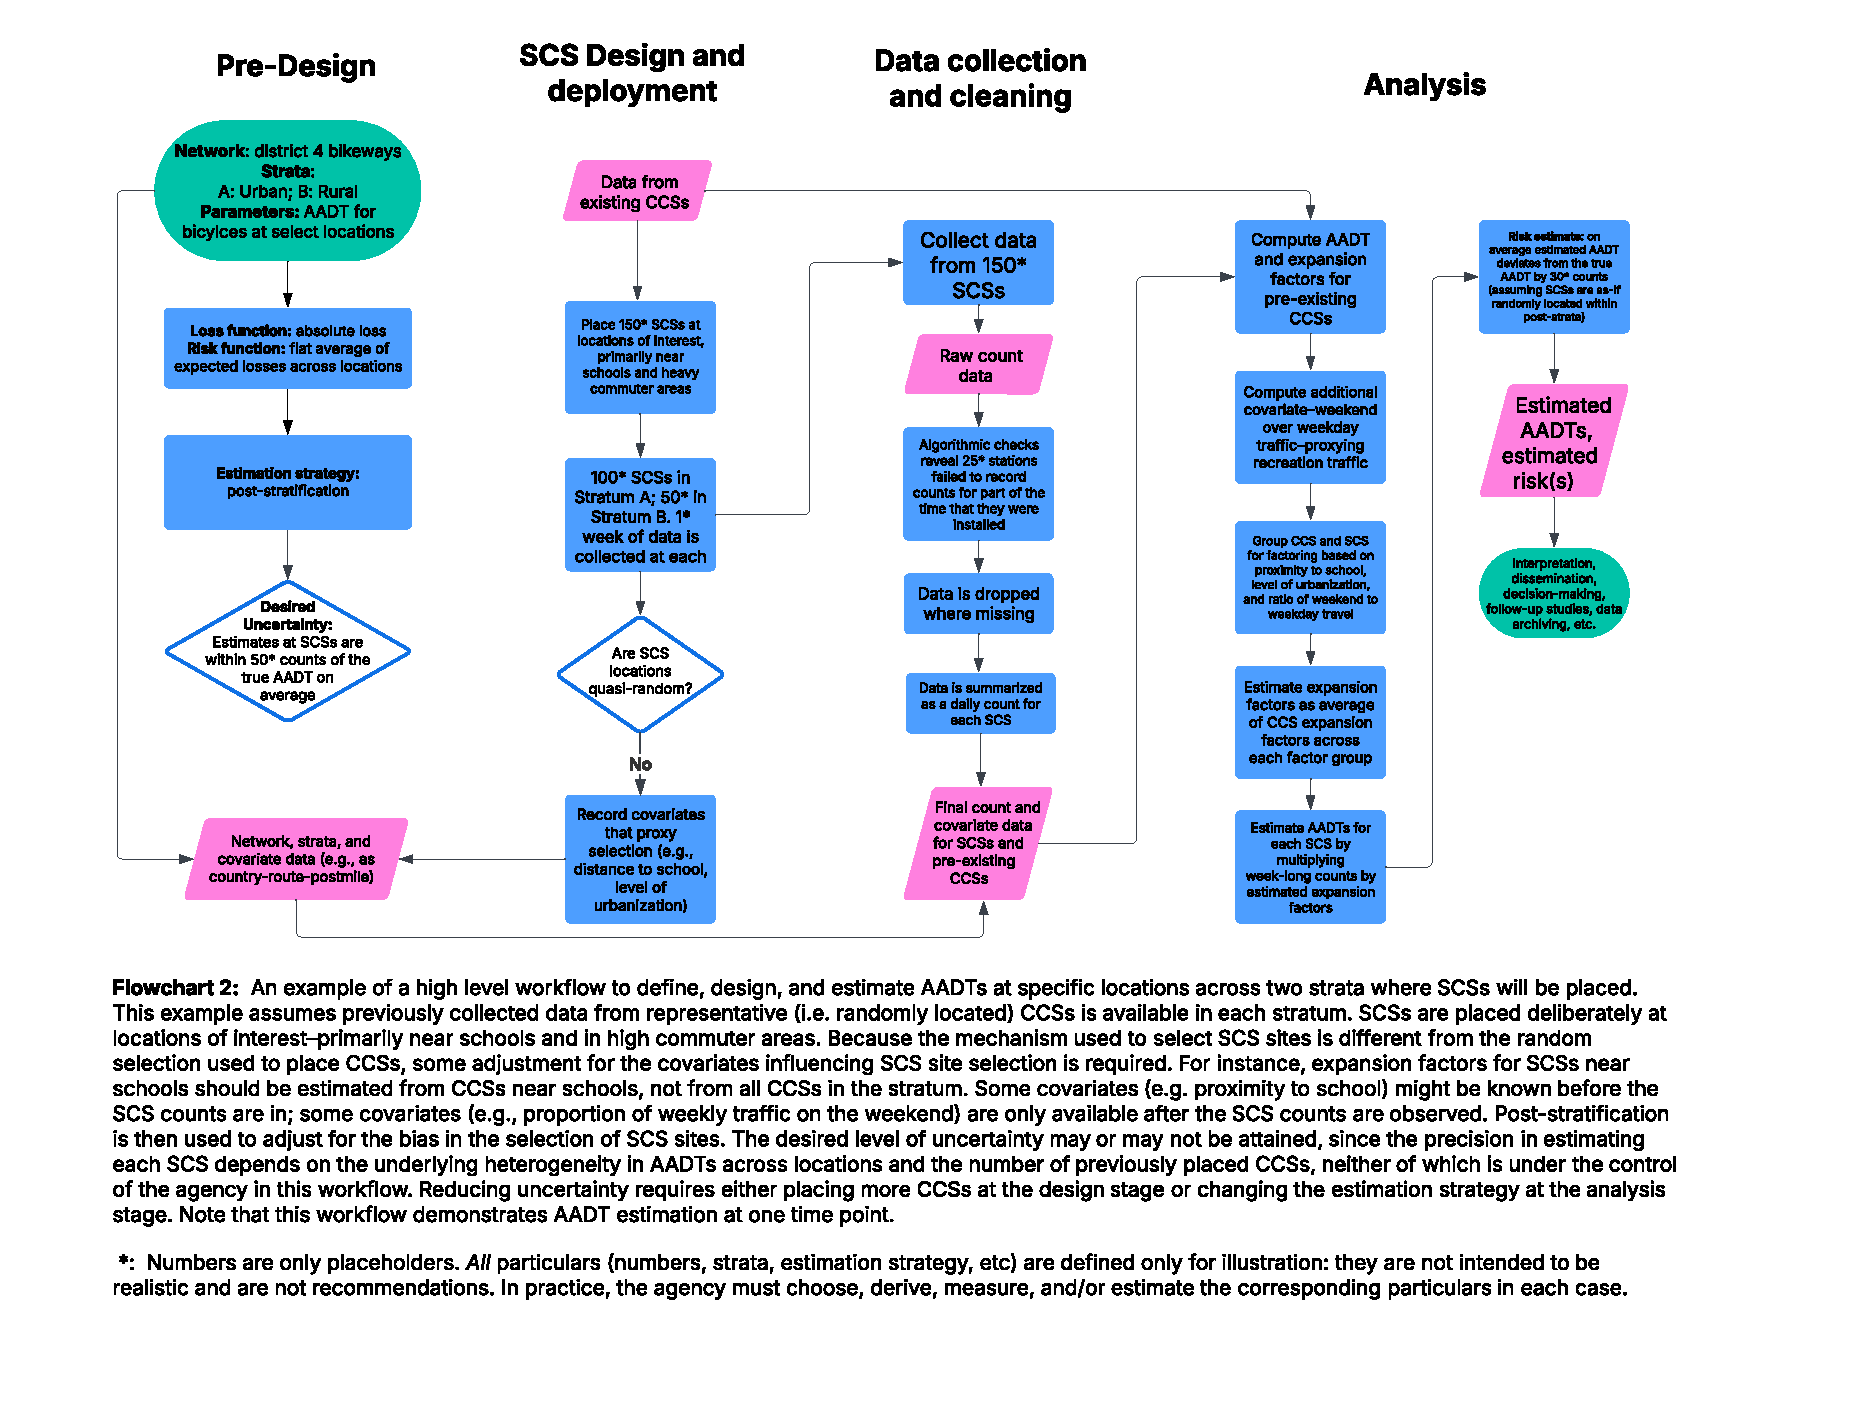
\includepdf[pages = 1]{../Output/Flowchart_example_2.pdf}


    \subsection{\texorpdfstring{Estimating AADT at the point \(r\) when
there is no station at
\(r\)}{Estimating AADT at the point r when there is no station at r}}\label{estimating-aadt-at-the-point-r-when-there-is-no-station-at-r}

Caltrans may wish to estimate an AADT \(\bar{y}(r)\) when \(r\) has
neither a CCS nor an SCS (we still assume that \(r\) is in a
\emph{stratum} where there are CCS counts).\\
To put it bluntly, \textbf{there is no way to do this without making
additional assumptions that may or may not be reasonable}. Those
assumptions come in two flavors: (1) the location of \(r\) is
essentially random, or (2) at the point \(r\), the AADT \(\bar{y}(r)\)
is essentially randomly distributed in a manner similar to the
distribution of the data at the CCSs.

Assumption (1) is questionable because the location \(r\) typically will
not be random: the agency does not choose where to make AADT estimates
as if by throwing darts at a map. As with AADT estimation at an SCS, the
agency must consider whether it is reasonable to treat the location
\emph{as if} it were random. If features of the location that led
Caltrans to want to estimate AADT there might be associated with AADT,
that assumption is shaky. Examples of such features include unusually
high population density, a history of traffic fatalities, proximity to a
public transit hub, etc. Assumption (2) is typically even more strained.
Especially for AT, AADT can vary across space in a highly idiosyncratic
and discontinuous fashion that is sensitive to local particulars and not
well modeled as a random draw from common probability distributions
(Gaussian, Poisson, zero-inflated binomial, etc). For this reason, we
suggest the agency record features that influence selection, adjust for
the influence of those features where possible to reduce bias, and be
aware of the propensity for AADT estimates made in this way to have
large biases.

Features that influence both selection and AADT are \emph{confounders},
and will bias estimates at purposively chosen locations. Even very
simple estimates are subject to this bias. For instance, although the
mean of AADTs at randomly-located CCSs is guaranteed to be an unbiased
estimate of the A-AADT and in fact is an unbiased estimate of the AADT
at any \emph{random} location in the stratum, it is \textbf{not} an
unbiased estimate of the AADT at a purposively chosen location.

If relevant features are recorded as covariates, bias can be reduced by
post-stratification and other statistical techniques usually called
\emph{regression} or \emph{supervised learning}. In particular, we could
posit a model for AADT that claims that the AADT at location \(r\) is
some unknown function of the known covariates, plus an idiosyncratic
residual or error term that does not depend on the covariates. In
symbols we can write the model as
\[\bar{y}(r) = f(\mathbf{x}(r)) + \epsilon(r),\] where \(f\) is an
unknown (potentially non-linear or discontinuous) function of the
observed covariate vector \(\mathbf{x}(r)\) and \(\epsilon(r)\) is the
idiosyncratic deviation of site \(r\) from that function. An estimate
\(\hat{f}\) of the unknown function \(f\) can be used to estimate the
AADT \(\bar{y}(r)\) at \(r\) by plugging the covariates
\(\mathbf{x}(r)\) into \(\hat{f}\). In symbols, the estimate is written
\[\hat{\bar{y}}(r) := \hat{f}(\mathbf{x}(r)).\] There are no statistical
guarantees about the predictions unless we make assumptions about
\(\epsilon(r)\), e.g., the unrealistic assumption that \(\epsilon(r)\)
is drawn from a normal distribution with mean 0 and standard deviation
\(\sigma_\epsilon\) for all \(r\).

A very simple set of assumptions holds that (a) \(f\) is entirely
constant over the stratum and (b) the variation \(\epsilon(r)\) is
randomly drawn from a distribution with mean zero. Taken together, these
assumptions do not imply that AADT is exactly constant (which is
obviously untrue), but they do imply that AADT can be treated as
essentially random with a mean that does not vary systemtically over
geography or other features of the locations. Because AADT obviously
depends on many features of the network (e.g.~the type of
infrastructure, motor vehicle traffic, population density, etc), the
assumption is unrealistic. Nevertheless, if these assumptions hold, then
it follows that \(f = \bar{\bar{y}}\) (the true function \(f\) is just
equal to the true A-AADT), and furthermore the A-AADT estimate
\(\hat{\bar{\bar{y}}}\) is a good predictor of \(\bar{y}(r)\) at any
location \(r\). Let \(\mathcal{C} := \{r_i^c\}_{i=1}^{n_c}\) be the set
of all CCS locations, and recall that \(\bar{y}_{\mathcal{F}}\) is the
mean AADT of the locations in \(\mathcal{F}\). If the CCSs were randomly
selected, the mean of \emph{all} the CCS AADTs \(\bar{y}_{\mathcal{C}}\)
is known and, if \(f\) is indeed constant, is a good estimate of
\(\hat{f}\). Under that assumption, the location and any covariate
information is irrelevant: we estimate the AADT for any \(r\) to be
\(\bar{y}_{\mathcal{C}}\).

We might instead assume that \(f\) is a piecewise constant function of
the covariates; for instance, that \(f\) is the same for all bikepaths
in the same city but different between any two cities (locations outside
any city might all be lumped together and assumed equal). Then
post-stratification might be used to estimate \(f\). In particular, if
the stratum is partioned into post-strata, and the set \(\mathcal{C}_s\)
denotes CCS locations in post-stratum \(s\), then the
post-stratification estimate for any location in post-stratum \(s\)
would be the average of CCS counts across post-stratum \(s\):
\[\hat{\bar{y}}(r) := \bar{y}_{\mathcal{C}_s}.\] This estimate might
improve on the A-AADT estimate in terms of reducing the risk at \(r\).
It might be particularly accurate if location \(r\) can be treated as-if
it were a uniform random draw from the post-stratum, i.e.~if it is
indistinguishable from other locations in the post-stratum from the
point of view of the agency. This would be the case if, for instance,
the agency actually used the covariates (and only the covariates!) to
choose the location \(r\). In reality, it seems likely that \(r\) will
be chosen for reasons that are not entirely represented in the
covariates (e.g., because a manager with some local knowledge not
encoded in the database asked for the AADT at location \(r\), or because
new infrastructure is being planned at location \(r\)).

If we do not wish to assume that \(f\) is piecewise constant, other
supervised learning techniques should be used to estimate \(f\),
including linear regression (ordinary least squares), nearest neighbors,
random forests, boosting, neural networks, and so on. We will not
elaborate on these techniques here. The first order concern in AADT
estimate at points is selection bias, which requires careful scrutiny
and transparent estimation techniques to address. There is a premium on
simplicity. We leave it to future researchers to investigate the value
of more sophisticated estimation methods.

    \section{References}\label{references}

\begin{enumerate}
\def\labelenumi{\arabic{enumi}.}
\tightlist
\item
  Albright, David. 1991. ``History of Estimating and Evaluating Annual
  Traffic Volume Statistics.'' Transportation Research Record, no. 1305.
  https://trid.trb.org/View/365623.
\item
  Bhowmick, Debjit, Meead Saberi, Mark Stevenson, Jason Thompson, Meghan
  Winters, Trisalyn Nelson, Simone Zarpelon Leao, Sachith Seneviratne,
  Christopher Pettit, Hai L. Vu, Kerry Nice, Ben Beck. 2023. ``A
  Systematic Scoping Review of Methods for Estimating Link-Level
  Bicycling Volumes.'' Transport Reviews, July.
  https://www.tandfonline.com/doi/full/10.1080/01441647.2022.2147240.
\item
  Boukerche, Azzedine, and Jiahao Wang. 2020. ``Machine Learning-Based
  Traffic Prediction Models for Intelligent Transportation Systems.''
  Computer Networks 181. https://doi.org/10.1016/j.comnet.2020.107530.
\item
  Chen, Peng, Jiangping Zhou, and Feiyang Sun. 2017. ``Built Environment
  Determinants of Bicycle Volume: A Longitudinal Analysis.'' Journal of
  Transport and Land Use 10 (1). https://doi.org/10.5198/jtlu.2017.892.
\item
  Crawford, Kate. 2013. ``The Hidden Biases in Big Data.'' Harvard
  Business Review, April 1, 2013.
  https://hbr.org/2013/04/the-hidden-biases-in-big-data.
\item
  Davis, Gary A, and Trina Wicklatz. 2001. ``Sample-Based Estimation of
  Bicycle Miles Traveled (BMT).'' Report for the Minnesota Department of
  Transportation. MN/RC -- 2001-23.
  https://cts-d8resmod-prd.oit.umn.edu/pdf/mndot-2001-23.pdf
\item
  Drusch, Robert L. 1966. ``Estimating Annual Average Daily Traffic from
  Short-Term Traffic Counts.'' Highway Research Record.
  https://trid.trb.org/View/120596.
\item
  Ferster, Colin, Trisalyn Nelson, Karen Laberee, and Meghan Winters.
  2021. ``Mapping Bicycling Exposure and Safety Risk Using Strava
  Metro.'' Applied Geography 127.
  https://doi.org/10.1016/j.apgeog.2021.102388.
\item
  Glazer, Amanda, Philip B. Stark, Md. Mintu Miah, Krita Nordback, Julia
  B. Griswold, and Alexander Skabardonis ``Data checks for bicycle and
  pedestrian counts''. Poster presented at Transportation Research Board
  103rd Annual Meeting, Washington, DC, January 9, 2024.
  https://www.researchgate.net/publication/377362665\_DATA\_CHECKS\_FOR\_BICYCLE\_AND\_PEDESTRIAN\_COUNTS
\item
  Gupta, Mohit, Debjit Bhowmick, Meead Saberi, Shirui Pan, and Ben Beck.
  2024. ``Evaluating the Effects of Data Sparsity on the Link-Level
  Bicycling Volume Estimation: A Graph Convolutional Neural Network
  Approach.'' ArXiv preprint. https://doi.org/10.48550/arXiv.2410.08522.
\item
  Hankey, Steve, Greg Lindsey, Xize Wang, Jason Borah, Kristopher Hoff,
  Brad Utecht, and Zhiyi Xu. 2012. ``Estimating Use of Non-Motorized
  Infrastructure: Models of Bicycle and Pedestrian Traffic in
  Minneapolis, MN.'' Landscape and Urban Planning 107.
  https://doi.org/10.1016/j.landurbplan.2012.06.005.
\item
  James, Gareth, Daniela Witten, Trevor Hastie, Robert Tibshirani, and
  Jonathan Taylor. 2023. An Introduction to Statistical Learning: With
  Applications in Python. Springer.
  https://link.springer.com/book/10.1007/978-3-031-38747-0.
\item
  Li, Yaguang, Rose Yu, Cyrus Shahabi, and Yan Liu. 2018. ``Diffusion
  Convolutional Recurrent Neural Network: Data-Driven Traffic
  Forecasting.'' International Conference on Learning Representations
  (ICLR), 2018. https://openreview.net/forum?id=SJiHXGWAZ.
\item
  McNally, Michael G., James E. Marca, Craig R. Rindt, and Angela M.
  Koos. 2003. ``TRACER: In-Vehicle, GPS-Based Wireless Technology for
  Traffic Surveillance and Management.'' California PATH Research
  Report. UCB-ITS-PRR-2003-23.
  https://escholarship.org/uc/item/19f152mt.
\item
  Nordback, Krista. 2014. ``Guide to Bicycle \& Pedestrian Count
  Programs.'' Transportation Research and Education Center.
  https://trec.pdx.edu/sites/default/files/smol-IBPI\%20Guide\%20to\%20Bicycle\%20\%26\%20Pedestrian\%20Count\%20Programs\_final.pdf.
\item
  Nordback, Krista, Sirisha Kothuri, Miguel A. Figliozzi, Taylor
  Phillips, Carson Gorecki, Andrew Schrope, and Portland State
  University. 2016. ``Investigation of Bicycle and Pedestrian Continuous
  and Short Duration Count Technologies in Oregon\,: Final Report\,: SPR
  772.'' FHWA-OR-RD-16-15. https://rosap.ntl.bts.gov/view/dot/30956.
\item
  Nordback, Krista, and Michael Sellinger. 2014. ``Methods for
  Estimating Bicycling and Walking in Washington State.'' Report for The
  State of Washington Department of Transportation. WA-RD 828.1.
  https://www.wsdot.wa.gov/research/reports/fullreports/828.1.pdf.
\item
  Selala, M. K., and W. Musakwa. 2016. ``The Potential of Strava Data to
  Contribute in Non-Motorised Transport (NMT) Planning in
  Johannesburg.'' The International Archives of the Photogrammetry,
  Remote Sensing and Spatial Information Sciences.
  https://doi.org/10.5194/isprs-archives-XLI-B2-587-2016.
\item
  Strauss, Jillian, and Luis F. Miranda-Moreno. 2013. ``Spatial Modeling
  of Bicycle Activity at Signalized Intersections.'' Journal of
  Transport and Land Use 6. https://doi.org/10.5198/jtlu.v6i2.296.
\item
  Tillé, Yves, and Matthieu Wilhelm. 2017. ``Probability Sampling
  Designs: Principles for Choice of Design and Balancing.'' Statistical
  Science 32. https://doi.org/10.1214/16-STS606.
\item
  Tsapakis, Ioannis, Paul Anderson, Zihang Wei, Shawn Turner, Anik Das,
  Mark Hallenbeck, Ben Chen, and Elizabeth Stolz. 2024. Guide on Methods
  for Assigning Counts to Adjustment Factor Groups. National Academies
  Press. https://doi.org/10.17226/27925.
\item
  United States Department of Transportation Federal Highway
  Administration. 2024. ``Traffic Monitoring Guide.'' FHWA-PL-022-026.
  https://rosap.ntl.bts.gov/view/dot/74643.
\item
  United States Federal Highway Administration Office of Highway Policy
  Information. 2018. ``Traffic Data Computation Method: Pocket Guide.''
  FHWA-PL-18-027. https://rosap.ntl.bts.gov/view/dot/57335.
\item
  Venter, Zander S., Vegard Gundersen, Samantha L. Scott, and David N.
  Barton. 2023. ``Bias and Precision of Crowdsourced Recreational
  Activity Data from Strava.'' Landscape and Urban Planning 232.
  https://doi.org/10.1016/j.landurbplan.2023.104686.
\item
  Yu, Bing, Haoteng Yin, and Zhanxing Zhu. 2018. ``Spatio-Temporal Graph
  Convolutional Networks: A Deep Learning Framework for Traffic
  Forecasting.'' In Proceedings of the 27th International Joint
  Conference on Artificial Intelligence (IJCAI'18).
  https://dl.acm.org/doi/10.5555/3304222.3304273.
\end{enumerate}

    \section{Software}\label{software}

The following section provides software to accomplish a variety of
tasks including:

\begin{enumerate}
\def\labelenumi{\arabic{enumi}.}
\tightlist
\item
  Sample a set of CCSs and SCSs from a population partioned into strata.
\item
  Calculate AADT at a point with a CCS station
\item
  Estimate A-AADT
\item
  Estimate AADT at a point with an SCS location using expansion factors
\item
  Estimate the risk of AADT estimation at a randomly located SCS using
  cross-validation
\item
  Estimate AADT at a point where there is no station by using the A-AADT
  estimate or poststratification
\end{enumerate}

The functions are generic and in some cases can be applied as they are. 
However, the software will need to be edited by Caltrans: the workflow here is merely illustrative and not intended for immediate use. 
Inputs to functions and other aspects of the software workflow are sensitive to the context in which they will be used by Caltrans and need to be adapted accordingly. 
Adaptations of the code below might involve the agency's goals and error tolerances, the proper format of input and output data to integrate with agency workflows, writing a simpler user interface for use by workers unfamiliar with python code, and/or adding specific historical data that the agency could use inform sample sizes and other choices. 
In particular, the agency could write additional loss functions to fit with their goals, they might adapt the functions used to form factor groups in order implement and/or evaluate their prefered method, they might change data input and output formats to integrate with existing workflows, they might reorder sections of the software to simplify data input, or define wrapper functions or loops to iterate over more complex data structures (e.g. a network with multiple strata).  


We first load in necessary Python packages and define necessary
functions. We then demonstrate each task in order. Except for the first,
the tasks are demonstrated using data from bicycle counters in
California in 2019. The data was processed and prepared by Amanda Glazer
(\href{https://www.researchgate.net/publication/377362665_DATA_CHECKS_FOR_BICYCLE_AND_PEDESTRIAN_COUNTS}{Glazer
et al, 2024}).

    \subsection{Setup}\label{setup}

    \subsubsection{Load external packages}\label{load-external-packages}

    \begin{tcolorbox}[breakable, size=fbox, boxrule=1pt, pad at break*=1mm,colback=cellbackground, colframe=cellborder]
\prompt{In}{incolor}{1}{\boxspacing}
\begin{Verbatim}[commandchars=\\\{\}]
\PY{c+c1}{\PYZsh{} import necessary packages}

\PY{k+kn}{import} \PY{n+nn}{numpy} \PY{k}{as} \PY{n+nn}{np}
\PY{k+kn}{import} \PY{n+nn}{pandas} \PY{k}{as} \PY{n+nn}{pd}
\PY{k+kn}{import} \PY{n+nn}{scipy} \PY{k}{as} \PY{n+nn}{sp}
\PY{k+kn}{import} \PY{n+nn}{warnings}

\PY{c+c1}{\PYZsh{}suppress some warnings}

\PY{n}{warnings}\PY{o}{.}\PY{n}{filterwarnings}\PY{p}{(}\PY{l+s+s2}{\PYZdq{}}\PY{l+s+s2}{ignore}\PY{l+s+s2}{\PYZdq{}}\PY{p}{,} \PY{n}{message}\PY{o}{=}\PY{l+s+s2}{\PYZdq{}}\PY{l+s+s2}{numpy.dtype size changed}\PY{l+s+s2}{\PYZdq{}}\PY{p}{)}
\PY{n}{warnings}\PY{o}{.}\PY{n}{filterwarnings}\PY{p}{(}\PY{l+s+s2}{\PYZdq{}}\PY{l+s+s2}{ignore}\PY{l+s+s2}{\PYZdq{}}\PY{p}{,} \PY{n}{message}\PY{o}{=}\PY{l+s+s2}{\PYZdq{}}\PY{l+s+s2}{numpy.ufunc size changed}\PY{l+s+s2}{\PYZdq{}}\PY{p}{)}
\PY{n}{warnings}\PY{o}{.}\PY{n}{filterwarnings}\PY{p}{(}\PY{l+s+s1}{\PYZsq{}}\PY{l+s+s1}{ignore}\PY{l+s+s1}{\PYZsq{}}\PY{p}{,} \PY{l+s+s2}{\PYZdq{}}\PY{l+s+s2}{Intel MKL WARNING}\PY{l+s+s2}{\PYZdq{}}\PY{p}{)}
\end{Verbatim}
\end{tcolorbox}

    \begin{tcolorbox}[breakable, size=fbox, boxrule=1pt, pad at break*=1mm,colback=cellbackground, colframe=cellborder]
\prompt{In}{incolor}{2}{\boxspacing}
\begin{Verbatim}[commandchars=\\\{\}]
\PY{c+c1}{\PYZsh{} package versions}

\PY{n+nb}{print}\PY{p}{(}\PY{n}{sp}\PY{o}{.}\PY{n}{\PYZus{}\PYZus{}version\PYZus{}\PYZus{}}\PY{p}{)}
\PY{n+nb}{print}\PY{p}{(}\PY{n}{np}\PY{o}{.}\PY{n}{\PYZus{}\PYZus{}version\PYZus{}\PYZus{}}\PY{p}{)}
\PY{n+nb}{print}\PY{p}{(}\PY{n}{pd}\PY{o}{.}\PY{n}{\PYZus{}\PYZus{}version\PYZus{}\PYZus{}}\PY{p}{)}
\end{Verbatim}
\end{tcolorbox}

    \begin{Verbatim}[commandchars=\\\{\}]
1.14.1
2.2.0
2.2.3
    \end{Verbatim}

    \subsubsection{Load functions}\label{load-functions}

    \paragraph{Risk and loss}\label{risk-and-loss}

    \begin{tcolorbox}[breakable, size=fbox, boxrule=1pt, pad at break*=1mm,colback=cellbackground, colframe=cellborder]
\prompt{In}{incolor}{3}{\boxspacing}
\begin{Verbatim}[commandchars=\\\{\}]
\PY{c+c1}{\PYZsh{} tools to estimate risk empirically}

\PY{k}{def} \PY{n+nf}{sample\PYZus{}loss}\PY{p}{(}\PY{n}{true}\PY{p}{:} \PY{n}{np}\PY{o}{.}\PY{n}{array}\PY{o}{=}\PY{k+kc}{None}\PY{p}{,} \PY{n}{predicted}\PY{p}{:} \PY{n}{np}\PY{o}{.}\PY{n}{array}\PY{o}{=}\PY{k+kc}{None}\PY{p}{,} \PY{n}{loss\PYZus{}func}\PY{p}{:} \PY{n+nb}{callable}\PY{o}{=}\PY{k+kc}{None}\PY{p}{,} \PY{n}{weights}\PY{p}{:} \PY{n}{np}\PY{o}{.}\PY{n}{array} \PY{o}{=} \PY{k+kc}{None}\PY{p}{)} \PY{o}{\PYZhy{}}\PY{o}{\PYZgt{}} \PY{n+nb}{float}\PY{p}{:}
\PY{+w}{    }\PY{l+s+sd}{\PYZsq{}\PYZsq{}\PYZsq{}}
\PY{l+s+sd}{    compute the loss function for estimated AADT(s) when the truth is known; aggregate by averaging if multiple AADTs are passed}
\PY{l+s+sd}{    this is the loss for a single sample. The true \PYZdq{}risk\PYZdq{} is defined as an expected value involving the design}
\PY{l+s+sd}{    this function can be used to estimate the true risk by simulation, resampling, cross\PYZhy{}validation, etc}
\PY{l+s+sd}{    }
\PY{l+s+sd}{    parameters}
\PY{l+s+sd}{    \PYZhy{}\PYZhy{}\PYZhy{}\PYZhy{}\PYZhy{}\PYZhy{}\PYZhy{}\PYZhy{}\PYZhy{}\PYZhy{}}
\PY{l+s+sd}{        true: np.array of n\PYZus{}s floats, where n\PYZus{}s is the number of short\PYZhy{}term stations}
\PY{l+s+sd}{            the true values}
\PY{l+s+sd}{        predicted: length\PYZhy{}n\PYZus{}s np.array of floats}
\PY{l+s+sd}{            the predicted values}
\PY{l+s+sd}{        loss\PYZus{}func: callable}
\PY{l+s+sd}{            the loss function }
\PY{l+s+sd}{        weights: length\PYZhy{}n\PYZus{}s np.array }
\PY{l+s+sd}{            optional vector of weights that sum to 1, defaults to 1/n\PYZus{}s}
\PY{l+s+sd}{            }
\PY{l+s+sd}{    returns}
\PY{l+s+sd}{    \PYZhy{}\PYZhy{}\PYZhy{}\PYZhy{}\PYZhy{}\PYZhy{}\PYZhy{}}
\PY{l+s+sd}{        a float representing the risk}
\PY{l+s+sd}{    \PYZsq{}\PYZsq{}\PYZsq{}}
    \PY{n}{n\PYZus{}s} \PY{o}{=} \PY{n+nb}{len}\PY{p}{(}\PY{n}{predicted}\PY{p}{)}
    \PY{n}{weights} \PY{o}{=} \PY{p}{(} \PY{n}{weights} \PY{k}{if} \PY{n}{weights} \PY{o+ow}{is} \PY{o+ow}{not} \PY{k+kc}{None} 
                \PY{k}{else} \PY{p}{(}\PY{l+m+mi}{1}\PY{o}{/}\PY{n}{n\PYZus{}s}\PY{p}{)}\PY{o}{*}\PY{n}{np}\PY{o}{.}\PY{n}{ones\PYZus{}like}\PY{p}{(}\PY{n}{predicted}\PY{p}{)}
              \PY{p}{)}
    \PY{k}{assert} \PY{n+nb}{len}\PY{p}{(}\PY{n}{weights}\PY{p}{)} \PY{o}{==} \PY{n}{n\PYZus{}s}\PY{p}{,} \PY{l+s+s2}{\PYZdq{}}\PY{l+s+s2}{Length of weights does not equal length of predictions}\PY{l+s+s2}{\PYZdq{}}
    \PY{k}{return} \PY{n}{np}\PY{o}{.}\PY{n}{sum}\PY{p}{(}\PY{n}{weights} \PY{o}{*} \PY{n}{loss\PYZus{}func}\PY{p}{(}\PY{n}{true}\PY{p}{,} \PY{n}{predicted}\PY{p}{)}\PY{p}{)}

\PY{c+c1}{\PYZsh{} some componentwise loss functions}
\PY{k}{def} \PY{n+nf}{squared\PYZus{}error\PYZus{}loss}\PY{p}{(}\PY{n}{true}\PY{p}{,} \PY{n}{predicted}\PY{p}{)}\PY{p}{:}
    \PY{k}{return} \PY{p}{(}\PY{n}{true} \PY{o}{\PYZhy{}} \PY{n}{predicted}\PY{p}{)}\PY{o}{*}\PY{o}{*}\PY{l+m+mi}{2}
    
\PY{k}{def} \PY{n+nf}{proportional\PYZus{}loss}\PY{p}{(}\PY{n}{true}\PY{p}{,} \PY{n}{predicted}\PY{p}{)}\PY{p}{:}
    \PY{k}{return} \PY{n}{np}\PY{o}{.}\PY{n}{abs}\PY{p}{(}\PY{n}{true} \PY{o}{\PYZhy{}} \PY{n}{predicted}\PY{p}{)} \PY{o}{/} \PY{n}{true}


\PY{c+c1}{\PYZsh{} unit tests}
\PY{c+c1}{\PYZsh{} sample loss}
\PY{n}{true} \PY{o}{=} \PY{n}{np}\PY{o}{.}\PY{n}{array}\PY{p}{(}\PY{p}{[}\PY{l+m+mi}{1}\PY{p}{]}\PY{p}{)}
\PY{n}{predicted} \PY{o}{=} \PY{n}{np}\PY{o}{.}\PY{n}{array}\PY{p}{(}\PY{p}{[}\PY{l+m+mi}{1}\PY{p}{]}\PY{p}{)}
\PY{k}{assert} \PY{n}{sample\PYZus{}loss}\PY{p}{(}\PY{n}{true}\PY{p}{,} \PY{n}{predicted}\PY{p}{,} \PY{n}{squared\PYZus{}error\PYZus{}loss}\PY{p}{)} \PY{o}{==} \PY{l+m+mi}{0}
\PY{k}{assert} \PY{n}{sample\PYZus{}loss}\PY{p}{(}\PY{n}{true}\PY{p}{,} \PY{n}{predicted}\PY{p}{,} \PY{n}{proportional\PYZus{}loss}\PY{p}{)} \PY{o}{==} \PY{l+m+mi}{0}
\PY{n}{true} \PY{o}{=} \PY{n}{np}\PY{o}{.}\PY{n}{array}\PY{p}{(}\PY{p}{[}\PY{l+m+mi}{1}\PY{p}{,}\PY{l+m+mi}{2}\PY{p}{]}\PY{p}{)}
\PY{n}{predicted} \PY{o}{=} \PY{n}{np}\PY{o}{.}\PY{n}{array}\PY{p}{(}\PY{p}{[}\PY{l+m+mi}{1}\PY{p}{,}\PY{l+m+mi}{2}\PY{p}{]}\PY{p}{)}
\PY{k}{assert} \PY{n}{sample\PYZus{}loss}\PY{p}{(}\PY{n}{true}\PY{p}{,} \PY{n}{predicted}\PY{p}{,} \PY{n}{squared\PYZus{}error\PYZus{}loss}\PY{p}{)} \PY{o}{==} \PY{l+m+mi}{0}
\PY{k}{assert} \PY{n}{sample\PYZus{}loss}\PY{p}{(}\PY{n}{true}\PY{p}{,} \PY{n}{predicted}\PY{p}{,} \PY{n}{proportional\PYZus{}loss}\PY{p}{)} \PY{o}{==} \PY{l+m+mi}{0}
\end{Verbatim}
\end{tcolorbox}

    \paragraph{Factor groups}\label{factor-groups}

    \begin{tcolorbox}[breakable, size=fbox, boxrule=1pt, pad at break*=1mm,colback=cellbackground, colframe=cellborder]
\prompt{In}{incolor}{4}{\boxspacing}
\begin{Verbatim}[commandchars=\\\{\}]
\PY{k}{def} \PY{n+nf}{define\PYZus{}factor\PYZus{}groups\PYZus{}allgroups}\PY{p}{(}\PY{n}{n\PYZus{}s}\PY{p}{:} \PY{n+nb}{int}\PY{o}{=}\PY{k+kc}{None}\PY{p}{,} \PY{n}{n\PYZus{}c}\PY{p}{:} \PY{n+nb}{int}\PY{o}{=}\PY{k+kc}{None}\PY{p}{)} \PY{o}{\PYZhy{}}\PY{o}{\PYZgt{}} \PY{n+nb}{list}\PY{p}{:}
\PY{+w}{    }\PY{l+s+sd}{\PYZsq{}\PYZsq{}\PYZsq{}}
\PY{l+s+sd}{    returns a factor group F\PYZus{}i for each of the n\PYZus{}s SCSs; each factor group contains every CCS, i.e. |F\PYZus{}i| = n\PYZus{}c}
\PY{l+s+sd}{    }
\PY{l+s+sd}{    parameters}
\PY{l+s+sd}{    \PYZhy{}\PYZhy{}\PYZhy{}\PYZhy{}\PYZhy{}\PYZhy{}\PYZhy{}\PYZhy{}\PYZhy{}\PYZhy{}\PYZhy{}}
\PY{l+s+sd}{        n\PYZus{}s: int}
\PY{l+s+sd}{            the number of SCSs}
\PY{l+s+sd}{        n\PYZus{}c: int}
\PY{l+s+sd}{            the number of CCSs}
\PY{l+s+sd}{    returns}
\PY{l+s+sd}{    \PYZhy{}\PYZhy{}\PYZhy{}\PYZhy{}\PYZhy{}\PYZhy{}\PYZhy{}\PYZhy{}}
\PY{l+s+sd}{        a length\PYZhy{}n\PYZus{}s list of factor groups F\PYZus{}i, each one of which is [0,...,(n\PYZus{}c \PYZhy{} 1)], i.e. an index of all CCSs }
\PY{l+s+sd}{    \PYZsq{}\PYZsq{}\PYZsq{}}
    \PY{n}{F} \PY{o}{=} \PY{p}{[}\PY{n}{np}\PY{o}{.}\PY{n}{arange}\PY{p}{(}\PY{n}{n\PYZus{}c}\PY{p}{)}\PY{p}{]} \PY{o}{*} \PY{n}{n\PYZus{}s}
    \PY{k}{return} \PY{n}{F}
    
\PY{k}{def} \PY{n+nf}{define\PYZus{}factor\PYZus{}groups\PYZus{}poststratification}\PY{p}{(}\PY{n}{SCS\PYZus{}strata}\PY{p}{:} \PY{n}{np}\PY{o}{.}\PY{n}{array}\PY{o}{=}\PY{k+kc}{None}\PY{p}{,} \PY{n}{CCS\PYZus{}strata}\PY{p}{:} \PY{n}{np}\PY{o}{.}\PY{n}{array}\PY{o}{=}\PY{k+kc}{None}\PY{p}{)} \PY{o}{\PYZhy{}}\PY{o}{\PYZgt{}} \PY{n+nb}{list}\PY{p}{:}
\PY{+w}{    }\PY{l+s+sd}{\PYZsq{}\PYZsq{}\PYZsq{}}
\PY{l+s+sd}{    Construct a factor group for each SCS. The factor group for an SCS is the list of indices of CCSs in its post\PYZhy{}stratum}

\PY{l+s+sd}{    parameters}
\PY{l+s+sd}{    \PYZhy{}\PYZhy{}\PYZhy{}\PYZhy{}\PYZhy{}\PYZhy{}\PYZhy{}\PYZhy{}\PYZhy{}\PYZhy{}}
\PY{l+s+sd}{        SCS\PYZus{}strata: length\PYZhy{}n\PYZus{}s np.array of ints or strs}
\PY{l+s+sd}{            identifiers of the post\PYZhy{}strata to which the SCSs belong}
\PY{l+s+sd}{        CCS\PYZus{}strata: length\PYZhy{}n\PYZus{}c np.array of ints or strs}
\PY{l+s+sd}{            identifiers of the post\PYZhy{}strata to which CCSs belong}
\PY{l+s+sd}{            }
\PY{l+s+sd}{    returns}
\PY{l+s+sd}{    \PYZhy{}\PYZhy{}\PYZhy{}\PYZhy{}\PYZhy{}\PYZhy{}\PYZhy{}}
\PY{l+s+sd}{        list of np.arrays: a length\PYZhy{}n\PYZus{}s list of factor groups F\PYZus{}i, each of which is an np.array containing the }
\PY{l+s+sd}{        indices of the CCSs in the same poststratum as the SCS}
\PY{l+s+sd}{    \PYZsq{}\PYZsq{}\PYZsq{}}
    \PY{n}{F} \PY{o}{=} \PY{p}{[}\PY{p}{]}
    \PY{n}{n\PYZus{}c} \PY{o}{=} \PY{n+nb}{len}\PY{p}{(}\PY{n}{CCS\PYZus{}strata}\PY{p}{)}
    \PY{k}{for} \PY{n}{SCS\PYZus{}stratum} \PY{o+ow}{in} \PY{n}{SCS\PYZus{}strata}\PY{p}{:}
        \PY{n}{F\PYZus{}i} \PY{o}{=} \PY{n}{np}\PY{o}{.}\PY{n}{where}\PY{p}{(}\PY{n}{SCS\PYZus{}stratum} \PY{o}{==} \PY{n}{CCS\PYZus{}strata}\PY{p}{)}\PY{p}{[}\PY{l+m+mi}{0}\PY{p}{]}
        \PY{k}{if} \PY{n}{F\PYZus{}i}\PY{o}{.}\PY{n}{size} \PY{o}{==} \PY{l+m+mi}{0}\PY{p}{:}
            \PY{n}{F\PYZus{}i} \PY{o}{=} \PY{n}{np}\PY{o}{.}\PY{n}{arange}\PY{p}{(}\PY{n}{n\PYZus{}c}\PY{p}{)} \PY{c+c1}{\PYZsh{} if the SCS stratum is not in the CCSs, its factor group is all CCSs}
            \PY{n}{warnings}\PY{o}{.}\PY{n}{warn}\PY{p}{(}\PY{l+s+sa}{f}\PY{l+s+s1}{\PYZsq{}}\PY{l+s+s1}{SCS stratum }\PY{l+s+si}{\PYZob{}}\PY{n}{SCS\PYZus{}stratum}\PY{l+s+si}{\PYZcb{}}\PY{l+s+s1}{ contains no CCSs: using default factor group containing all CCSs.}\PY{l+s+s1}{\PYZsq{}}\PY{p}{)}
        \PY{n}{F}\PY{o}{.}\PY{n}{append}\PY{p}{(}\PY{n}{F\PYZus{}i}\PY{p}{)}
    \PY{k}{return} \PY{n}{F}


\PY{k}{def} \PY{n+nf}{define\PYZus{}factor\PYZus{}groups\PYZus{}nearestneighbor}\PY{p}{(}
        \PY{n}{SCS\PYZus{}X}\PY{p}{:} \PY{n}{np}\PY{o}{.}\PY{n}{array}\PY{o}{=}\PY{k+kc}{None}\PY{p}{,} \PY{n}{CCS\PYZus{}X}\PY{p}{:} \PY{n}{np}\PY{o}{.}\PY{n}{array}\PY{o}{=}\PY{k+kc}{None}\PY{p}{,} \PY{n}{K}\PY{p}{:} \PY{n+nb}{int}\PY{o}{=}\PY{k+kc}{None}\PY{p}{,} \PY{n}{distance}\PY{p}{:} \PY{n+nb}{str}\PY{o}{=}\PY{l+s+s1}{\PYZsq{}}\PY{l+s+s1}{mahalanobis}\PY{l+s+s1}{\PYZsq{}}\PY{p}{)} \PY{o}{\PYZhy{}}\PY{o}{\PYZgt{}} \PY{n+nb}{list}\PY{p}{:}
\PY{+w}{    }\PY{l+s+sd}{\PYZsq{}\PYZsq{}\PYZsq{}}
\PY{l+s+sd}{    Construct n\PYZus{}s factor groups, one for each SCS, comprising the K CCSs closest in covariate space in the pseudometric `distance`}

\PY{l+s+sd}{    Covariates are assumed to be float\PYZhy{}valued, so categorical covariates should be encoded using dummy variables.}

\PY{l+s+sd}{    parameters}
\PY{l+s+sd}{    \PYZhy{}\PYZhy{}\PYZhy{}\PYZhy{}\PYZhy{}\PYZhy{}\PYZhy{}\PYZhy{}\PYZhy{}\PYZhy{}}
\PY{l+s+sd}{        SCS\PYZus{}X: size\PYZhy{}(n\PYZus{}s, p) np.array (matrix) of floats}
\PY{l+s+sd}{            the covariate matrix for the SCSs}
\PY{l+s+sd}{        CCS\PYZus{}X: size\PYZhy{}(n\PYZus{}c, p) np.array of floats}
\PY{l+s+sd}{            the corresponding covariate matrix for the CCSs (columns must align with columns of SCS\PYZus{}X)}
\PY{l+s+sd}{        K: int}
\PY{l+s+sd}{            the number of nearest neighbors to match on, i.e. the desired size of each factor group}
\PY{l+s+sd}{        distance: str}
\PY{l+s+sd}{            the name of the distance function in covariate space for finding the nearest neighbors.}
\PY{l+s+sd}{            defaults to Mahalanobis distance}
\PY{l+s+sd}{            see the documentation for sp.spatial.distance.cdist for more information on distances that can be used}
\PY{l+s+sd}{            https://docs.scipy.org/doc/scipy/reference/generated/scipy.spatial.distance.cdist.html}
\PY{l+s+sd}{            }
\PY{l+s+sd}{    returns}
\PY{l+s+sd}{    \PYZhy{}\PYZhy{}\PYZhy{}\PYZhy{}\PYZhy{}\PYZhy{}\PYZhy{}}
\PY{l+s+sd}{        a length\PYZhy{}n\PYZus{}s list of factor groups F\PYZus{}i, one for each SCS, each of size K}
\PY{l+s+sd}{    \PYZsq{}\PYZsq{}\PYZsq{}}
    \PY{n}{dists} \PY{o}{=} \PY{n}{sp}\PY{o}{.}\PY{n}{spatial}\PY{o}{.}\PY{n}{distance}\PY{o}{.}\PY{n}{cdist}\PY{p}{(}\PY{n}{SCS\PYZus{}X}\PY{p}{,} \PY{n}{CCS\PYZus{}X}\PY{p}{,} \PY{n}{metric} \PY{o}{=} \PY{n}{distance}\PY{p}{)}   
    \PY{c+c1}{\PYZsh{} Get the indices of the K nearest neighbors for each row in SCS\PYZus{}X}
    \PY{n}{neighbors\PYZus{}indices} \PY{o}{=} \PY{n}{np}\PY{o}{.}\PY{n}{argsort}\PY{p}{(}\PY{n}{dists}\PY{p}{,} \PY{n}{axis}\PY{o}{=}\PY{l+m+mi}{1}\PY{p}{)}\PY{p}{[}\PY{p}{:}\PY{p}{,} \PY{p}{:}\PY{n}{K}\PY{p}{]}
    \PY{n}{F} \PY{o}{=} \PY{p}{[}\PY{n}{neighbors\PYZus{}indices}\PY{p}{[}\PY{n}{i}\PY{p}{,}\PY{p}{:}\PY{p}{]} \PY{k}{for} \PY{n}{i} \PY{o+ow}{in} \PY{n+nb}{range}\PY{p}{(}\PY{n}{neighbors\PYZus{}indices}\PY{o}{.}\PY{n}{shape}\PY{p}{[}\PY{l+m+mi}{0}\PY{p}{]}\PY{p}{)}\PY{p}{]}
    \PY{k}{return} \PY{n}{F}


\PY{c+c1}{\PYZsh{} unit tests}
\PY{c+c1}{\PYZsh{} test allgroups}
\PY{n}{F} \PY{o}{=} \PY{n}{define\PYZus{}factor\PYZus{}groups\PYZus{}allgroups}\PY{p}{(}\PY{n}{n\PYZus{}s} \PY{o}{=} \PY{l+m+mi}{1}\PY{p}{,} \PY{n}{n\PYZus{}c} \PY{o}{=} \PY{l+m+mi}{3}\PY{p}{)}
\PY{k}{assert} \PY{n}{np}\PY{o}{.}\PY{n}{all}\PY{p}{(}\PY{n}{F}\PY{p}{[}\PY{l+m+mi}{0}\PY{p}{]} \PY{o}{==} \PY{n}{np}\PY{o}{.}\PY{n}{array}\PY{p}{(}\PY{p}{[}\PY{l+m+mi}{0}\PY{p}{,}\PY{l+m+mi}{1}\PY{p}{,}\PY{l+m+mi}{2}\PY{p}{]}\PY{p}{)}\PY{p}{)}
\PY{n}{F} \PY{o}{=} \PY{n}{define\PYZus{}factor\PYZus{}groups\PYZus{}allgroups}\PY{p}{(}\PY{n}{n\PYZus{}s} \PY{o}{=} \PY{l+m+mi}{3}\PY{p}{,} \PY{n}{n\PYZus{}c} \PY{o}{=} \PY{l+m+mi}{3}\PY{p}{)}
\PY{k}{assert} \PY{n+nb}{all}\PY{p}{(}\PY{p}{[}\PY{n}{np}\PY{o}{.}\PY{n}{all}\PY{p}{(}\PY{n}{F}\PY{p}{[}\PY{n}{i}\PY{p}{]} \PY{o}{==} \PY{n}{np}\PY{o}{.}\PY{n}{array}\PY{p}{(}\PY{p}{[}\PY{l+m+mi}{0}\PY{p}{,}\PY{l+m+mi}{1}\PY{p}{,}\PY{l+m+mi}{2}\PY{p}{]}\PY{p}{)}\PY{p}{)} \PY{k}{for} \PY{n}{i} \PY{o+ow}{in} \PY{n+nb}{range}\PY{p}{(}\PY{l+m+mi}{3}\PY{p}{)}\PY{p}{]}\PY{p}{)}

\PY{c+c1}{\PYZsh{} test poststratification}
\PY{n}{scs\PYZus{}strata} \PY{o}{=} \PY{n}{np}\PY{o}{.}\PY{n}{array}\PY{p}{(}\PY{p}{[}\PY{l+s+s2}{\PYZdq{}}\PY{l+s+s2}{pear}\PY{l+s+s2}{\PYZdq{}}\PY{p}{,} \PY{l+s+s2}{\PYZdq{}}\PY{l+s+s2}{apple}\PY{l+s+s2}{\PYZdq{}}\PY{p}{]}\PY{p}{)}
\PY{n}{ccs\PYZus{}strata} \PY{o}{=} \PY{n}{np}\PY{o}{.}\PY{n}{array}\PY{p}{(}\PY{p}{[}\PY{l+s+s2}{\PYZdq{}}\PY{l+s+s2}{pear}\PY{l+s+s2}{\PYZdq{}}\PY{p}{,} \PY{l+s+s2}{\PYZdq{}}\PY{l+s+s2}{pear}\PY{l+s+s2}{\PYZdq{}}\PY{p}{,} \PY{l+s+s2}{\PYZdq{}}\PY{l+s+s2}{apple}\PY{l+s+s2}{\PYZdq{}}\PY{p}{]}\PY{p}{)}
\PY{n}{F} \PY{o}{=} \PY{n}{define\PYZus{}factor\PYZus{}groups\PYZus{}poststratification}\PY{p}{(}\PY{n}{SCS\PYZus{}strata} \PY{o}{=} \PY{n}{scs\PYZus{}strata}\PY{p}{,} \PY{n}{CCS\PYZus{}strata} \PY{o}{=} \PY{n}{ccs\PYZus{}strata}\PY{p}{)}
\PY{k}{assert} \PY{n}{np}\PY{o}{.}\PY{n}{all}\PY{p}{(}\PY{n}{F}\PY{p}{[}\PY{l+m+mi}{0}\PY{p}{]} \PY{o}{==} \PY{n}{np}\PY{o}{.}\PY{n}{array}\PY{p}{(}\PY{p}{[}\PY{l+m+mi}{0}\PY{p}{,}\PY{l+m+mi}{1}\PY{p}{]}\PY{p}{)}\PY{p}{)}
\PY{k}{assert} \PY{n}{np}\PY{o}{.}\PY{n}{all}\PY{p}{(}\PY{n}{F}\PY{p}{[}\PY{l+m+mi}{1}\PY{p}{]} \PY{o}{==} \PY{n}{np}\PY{o}{.}\PY{n}{array}\PY{p}{(}\PY{p}{[}\PY{l+m+mi}{2}\PY{p}{]}\PY{p}{)}\PY{p}{)}

\PY{c+c1}{\PYZsh{} test nearest neighbors}
\PY{n}{X\PYZus{}scs} \PY{o}{=} \PY{n}{np}\PY{o}{.}\PY{n}{array}\PY{p}{(}\PY{p}{[}\PY{p}{[}\PY{l+m+mf}{0.}\PY{p}{,}\PY{l+m+mi}{0}\PY{p}{]}\PY{p}{,} \PY{p}{[}\PY{l+m+mi}{1}\PY{p}{,}\PY{l+m+mi}{1}\PY{p}{]}\PY{p}{,} \PY{p}{[}\PY{l+m+mi}{1}\PY{p}{,}\PY{l+m+mi}{0}\PY{p}{]}\PY{p}{]}\PY{p}{)}
\PY{n}{X\PYZus{}ccs} \PY{o}{=} \PY{n}{np}\PY{o}{.}\PY{n}{array}\PY{p}{(}\PY{p}{[}\PY{p}{[}\PY{l+m+mf}{0.}\PY{p}{,}\PY{l+m+mi}{0}\PY{p}{]}\PY{p}{,} \PY{p}{[}\PY{l+m+mi}{1}\PY{p}{,}\PY{l+m+mi}{1}\PY{p}{]}\PY{p}{]}\PY{p}{)}
\PY{n}{F} \PY{o}{=} \PY{n}{define\PYZus{}factor\PYZus{}groups\PYZus{}nearestneighbor}\PY{p}{(}\PY{n}{SCS\PYZus{}X} \PY{o}{=} \PY{n}{X\PYZus{}scs}\PY{p}{,} \PY{n}{CCS\PYZus{}X} \PY{o}{=} \PY{n}{X\PYZus{}ccs}\PY{p}{,} \PY{n}{K} \PY{o}{=} \PY{l+m+mi}{1}\PY{p}{)}
\PY{k}{assert} \PY{n}{np}\PY{o}{.}\PY{n}{all}\PY{p}{(}\PY{n}{F}\PY{p}{[}\PY{l+m+mi}{0}\PY{p}{]} \PY{o}{==} \PY{n}{np}\PY{o}{.}\PY{n}{array}\PY{p}{(}\PY{p}{[}\PY{l+m+mi}{0}\PY{p}{]}\PY{p}{)}\PY{p}{)}
\PY{k}{assert} \PY{n}{np}\PY{o}{.}\PY{n}{all}\PY{p}{(}\PY{n}{F}\PY{p}{[}\PY{l+m+mi}{1}\PY{p}{]} \PY{o}{==} \PY{n}{np}\PY{o}{.}\PY{n}{array}\PY{p}{(}\PY{p}{[}\PY{l+m+mi}{1}\PY{p}{]}\PY{p}{)}\PY{p}{)}
\PY{n}{F} \PY{o}{=} \PY{n}{define\PYZus{}factor\PYZus{}groups\PYZus{}nearestneighbor}\PY{p}{(}\PY{n}{SCS\PYZus{}X} \PY{o}{=} \PY{n}{X\PYZus{}scs}\PY{p}{,} \PY{n}{CCS\PYZus{}X} \PY{o}{=} \PY{n}{X\PYZus{}ccs}\PY{p}{,} \PY{n}{K} \PY{o}{=} \PY{l+m+mi}{2}\PY{p}{)}
\PY{k}{assert} \PY{n}{np}\PY{o}{.}\PY{n}{all}\PY{p}{(}\PY{n}{F}\PY{p}{[}\PY{l+m+mi}{0}\PY{p}{]} \PY{o}{==} \PY{n}{np}\PY{o}{.}\PY{n}{array}\PY{p}{(}\PY{p}{[}\PY{l+m+mi}{0}\PY{p}{,} \PY{l+m+mi}{1}\PY{p}{]}\PY{p}{)}\PY{p}{)}
\PY{k}{assert} \PY{n}{np}\PY{o}{.}\PY{n}{all}\PY{p}{(}\PY{n}{F}\PY{p}{[}\PY{l+m+mi}{1}\PY{p}{]} \PY{o}{==} \PY{n}{np}\PY{o}{.}\PY{n}{array}\PY{p}{(}\PY{p}{[}\PY{l+m+mi}{1}\PY{p}{,} \PY{l+m+mi}{0}\PY{p}{]}\PY{p}{)}\PY{p}{)}
\end{Verbatim}
\end{tcolorbox}

    \paragraph{Form CCS expansion factors}\label{form-ccs-expansion-factors}

    \begin{tcolorbox}[breakable, size=fbox, boxrule=1pt, pad at break*=1mm,colback=cellbackground, colframe=cellborder]
\prompt{In}{incolor}{5}{\boxspacing}
\begin{Verbatim}[commandchars=\\\{\}]
\PY{k}{def} \PY{n+nf}{estimate\PYZus{}expansion\PYZus{}factors}\PY{p}{(}\PY{n}{F\PYZus{}i}\PY{p}{:} \PY{n}{np}\PY{o}{.}\PY{n}{array}\PY{o}{=}\PY{k+kc}{None}\PY{p}{,} \PY{n}{y\PYZus{}c}\PY{p}{:} \PY{n}{np}\PY{o}{.}\PY{n}{array}\PY{o}{=}\PY{k+kc}{None}\PY{p}{,} \PY{n}{factor\PYZus{}method}\PY{p}{:} \PY{n+nb}{str}\PY{o}{=}\PY{l+s+s2}{\PYZdq{}}\PY{l+s+s2}{averaging}\PY{l+s+s2}{\PYZdq{}}\PY{p}{)} \PY{o}{\PYZhy{}}\PY{o}{\PYZgt{}} \PY{n}{np}\PY{o}{.}\PY{n}{array}\PY{p}{:}
\PY{+w}{    }\PY{l+s+sd}{\PYZsq{}\PYZsq{}\PYZsq{}}
\PY{l+s+sd}{    estimate expansion factors for factor group F\PYZus{}i from matrix of CCS counts y\PYZus{}c }
\PY{l+s+sd}{    }
\PY{l+s+sd}{    parameters}
\PY{l+s+sd}{    \PYZhy{}\PYZhy{}\PYZhy{}\PYZhy{}\PYZhy{}\PYZhy{}\PYZhy{}\PYZhy{}\PYZhy{}\PYZhy{}\PYZhy{}\PYZhy{}\PYZhy{}}
\PY{l+s+sd}{        F\PYZus{}i: np.array of ints}
\PY{l+s+sd}{            the indices of the factor group for SCS i in the set of CCSs}
\PY{l+s+sd}{            e.g., 1,...,n\PYZus{}c corresponds to all CCSs}
\PY{l+s+sd}{        y\PYZus{}c: size\PYZhy{}(n\PYZus{}c, t\PYZus{}max) np.array (i.e., a matrix)}
\PY{l+s+sd}{            the complete counts for all CCSs}
\PY{l+s+sd}{        factor\PYZus{}method: str in [\PYZdq{}averaging\PYZdq{}, \PYZdq{}ratio\PYZdq{}]}
\PY{l+s+sd}{            the method used to compute the expansion factor}
\PY{l+s+sd}{            \PYZdq{}averaging\PYZdq{} sets w\PYZus{}i for week t to the average of the n\PYZus{}c expansion factors for week t across all CCSs in F\PYZus{}i }
\PY{l+s+sd}{             \PYZdq{}ratio\PYZdq{} sets w\PYZus{}i for week t to the total annual count across all CCSs in F\PYZus{}i divided by the total count }
\PY{l+s+sd}{                 across all CCSs in F\PYZus{}i in week t; it is not recommended at this time}
\PY{l+s+sd}{    returns:}
\PY{l+s+sd}{    \PYZhy{}\PYZhy{}\PYZhy{}\PYZhy{}\PYZhy{}\PYZhy{}\PYZhy{}\PYZhy{}}
\PY{l+s+sd}{        length\PYZhy{}t\PYZus{}max np.array, the expansion factors for factor group F\PYZus{}i}
\PY{l+s+sd}{    \PYZsq{}\PYZsq{}\PYZsq{}}
    \PY{n}{days\PYZus{}per\PYZus{}year} \PY{o}{=} \PY{l+m+mi}{365}
    \PY{n}{y\PYZus{}F\PYZus{}i} \PY{o}{=} \PY{n}{y\PYZus{}c}\PY{p}{[}\PY{n}{F\PYZus{}i}\PY{p}{,}\PY{p}{:}\PY{p}{]} \PY{c+c1}{\PYZsh{} all CCS counts in factor group F\PYZus{}i}
    \PY{k}{if} \PY{n}{factor\PYZus{}method} \PY{o}{==} \PY{l+s+s2}{\PYZdq{}}\PY{l+s+s2}{ratio}\PY{l+s+s2}{\PYZdq{}}\PY{p}{:}
        \PY{n}{AADT\PYZus{}bar} \PY{o}{=} \PY{n}{np}\PY{o}{.}\PY{n}{mean}\PY{p}{(}\PY{p}{(}\PY{l+m+mi}{1}\PY{o}{/}\PY{n}{days\PYZus{}per\PYZus{}year}\PY{p}{)} \PY{o}{*} \PY{n}{np}\PY{o}{.}\PY{n}{sum}\PY{p}{(}\PY{n}{y\PYZus{}F\PYZus{}i}\PY{p}{,} \PY{n}{axis} \PY{o}{=} \PY{l+m+mi}{1}\PY{p}{)}\PY{p}{)} \PY{c+c1}{\PYZsh{} average AADT across all CCSs in factor group F\PYZus{}i}
        \PY{n}{week\PYZus{}avg} \PY{o}{=} \PY{n}{np}\PY{o}{.}\PY{n}{mean}\PY{p}{(}\PY{n}{y\PYZus{}F\PYZus{}i}\PY{p}{,} \PY{n}{axis} \PY{o}{=} \PY{l+m+mi}{0}\PY{p}{)} \PY{c+c1}{\PYZsh{} average weekly counts across CCSs in factor group F\PYZus{}i}
        \PY{n}{w\PYZus{}it} \PY{o}{=} \PY{n}{AADT\PYZus{}bar} \PY{o}{/} \PY{n}{week\PYZus{}avg} \PY{c+c1}{\PYZsh{} ratio expansion factors}
    \PY{k}{elif} \PY{n}{factor\PYZus{}method} \PY{o}{==} \PY{l+s+s2}{\PYZdq{}}\PY{l+s+s2}{averaging}\PY{l+s+s2}{\PYZdq{}}\PY{p}{:}
        \PY{n}{AADT\PYZus{}F\PYZus{}i} \PY{o}{=} \PY{p}{(}\PY{l+m+mi}{1}\PY{o}{/}\PY{n}{days\PYZus{}per\PYZus{}year}\PY{p}{)} \PY{o}{*} \PY{n}{y\PYZus{}F\PYZus{}i}\PY{o}{.}\PY{n}{sum}\PY{p}{(}\PY{n}{axis} \PY{o}{=} \PY{l+m+mi}{1}\PY{p}{,} \PY{n}{keepdims} \PY{o}{=} \PY{k+kc}{True}\PY{p}{)} \PY{c+c1}{\PYZsh{} AADTs for CCSs in group F\PYZus{}i}
        \PY{n}{w\PYZus{}F\PYZus{}i} \PY{o}{=} \PY{n}{AADT\PYZus{}F\PYZus{}i} \PY{o}{/} \PY{n}{y\PYZus{}F\PYZus{}i} \PY{c+c1}{\PYZsh{} expansion factors for each week and each CCS in group F\PYZus{}i}
        \PY{n}{w\PYZus{}it} \PY{o}{=} \PY{n}{np}\PY{o}{.}\PY{n}{mean}\PY{p}{(}\PY{n}{w\PYZus{}F\PYZus{}i}\PY{p}{,} \PY{n}{axis} \PY{o}{=} \PY{l+m+mi}{0}\PY{p}{)} \PY{c+c1}{\PYZsh{} averaging expansion factors}
    \PY{k}{else}\PY{p}{:} 
        \PY{k}{raise} \PY{n+ne}{ValueError}\PY{p}{(}\PY{l+s+s2}{\PYZdq{}}\PY{l+s+s2}{Invalid value for factor\PYZus{}method argument; must be }\PY{l+s+s2}{\PYZsq{}}\PY{l+s+s2}{ratio}\PY{l+s+s2}{\PYZsq{}}\PY{l+s+s2}{ or }\PY{l+s+s2}{\PYZsq{}}\PY{l+s+s2}{averaging}\PY{l+s+s2}{\PYZsq{}}\PY{l+s+s2}{\PYZdq{}}\PY{p}{)} 
    \PY{k}{return} \PY{n}{w\PYZus{}it} 

\PY{k}{def} \PY{n+nf}{estimate\PYZus{}all\PYZus{}expansion\PYZus{}factors}\PY{p}{(}\PY{n}{F}\PY{p}{:} \PY{n+nb}{list}\PY{o}{=}\PY{k+kc}{None}\PY{p}{,} \PY{n}{y\PYZus{}c}\PY{p}{:} \PY{n}{np}\PY{o}{.}\PY{n}{array}\PY{o}{=}\PY{k+kc}{None}\PY{p}{,} \PY{n}{factor\PYZus{}method}\PY{p}{:} \PY{n+nb}{str}\PY{o}{=}\PY{l+s+s1}{\PYZsq{}}\PY{l+s+s1}{averaging}\PY{l+s+s1}{\PYZsq{}}\PY{p}{)} \PY{o}{\PYZhy{}}\PY{o}{\PYZgt{}} \PY{n}{np}\PY{o}{.}\PY{n}{array}\PY{p}{:}
\PY{+w}{    }\PY{l+s+sd}{\PYZsq{}\PYZsq{}\PYZsq{}}
\PY{l+s+sd}{    wrapper for estimate\PYZus{}expansion\PYZus{}factors: estimate all expansion factors for factor groups in F from matrix of CCS counts y\PYZus{}c }
\PY{l+s+sd}{   }
\PY{l+s+sd}{    parameters}
\PY{l+s+sd}{    \PYZhy{}\PYZhy{}\PYZhy{}\PYZhy{}\PYZhy{}\PYZhy{}\PYZhy{}\PYZhy{}\PYZhy{}\PYZhy{}\PYZhy{}\PYZhy{}}
\PY{l+s+sd}{        F\PYZus{}i: list of np.arrays of ints}
\PY{l+s+sd}{            the indices in the set of CCSs for the factor group for each SCS i in 1...n\PYZus{}s}
\PY{l+s+sd}{        y\PYZus{}c: size\PYZhy{}(n\PYZus{}c, t\PYZus{}max) np.array (i.e., a matrix)}
\PY{l+s+sd}{            the complete counts for all CCSs}
\PY{l+s+sd}{            the method used to compute the expansion factor}
\PY{l+s+sd}{            \PYZdq{}averaging\PYZdq{} sets w\PYZus{}i for week t to the average of the n\PYZus{}c expansion factors for week t across all CCSs in F\PYZus{}i }
\PY{l+s+sd}{            \PYZdq{}ratio\PYZdq{} sets w\PYZus{}i for week t to the total annual count across all CCSs in F\PYZus{}i divided by the total count }
\PY{l+s+sd}{                 across all CCSs in F\PYZus{}i in week t; it is not recommended at this time}
\PY{l+s+sd}{    returns}
\PY{l+s+sd}{    \PYZhy{}\PYZhy{}\PYZhy{}\PYZhy{}\PYZhy{}\PYZhy{}\PYZhy{}}
\PY{l+s+sd}{        length\PYZhy{}t\PYZus{}max np.array, the expansion factors for factor group F\PYZus{}i}
\PY{l+s+sd}{    \PYZsq{}\PYZsq{}\PYZsq{}}
    \PY{n}{t\PYZus{}max} \PY{o}{=} \PY{n}{y\PYZus{}c}\PY{o}{.}\PY{n}{shape}\PY{p}{[}\PY{l+m+mi}{1}\PY{p}{]}
    \PY{n}{n\PYZus{}s} \PY{o}{=} \PY{n+nb}{len}\PY{p}{(}\PY{n}{F}\PY{p}{)}
    \PY{n}{w} \PY{o}{=} \PY{n}{np}\PY{o}{.}\PY{n}{zeros}\PY{p}{(}\PY{p}{(}\PY{n}{n\PYZus{}s}\PY{p}{,} \PY{n}{t\PYZus{}max}\PY{p}{)}\PY{p}{)}
    \PY{k}{for} \PY{n}{i} \PY{o+ow}{in} \PY{n+nb}{range}\PY{p}{(}\PY{n}{n\PYZus{}s}\PY{p}{)}\PY{p}{:}
        \PY{n}{w}\PY{p}{[}\PY{n}{i}\PY{p}{,}\PY{p}{:}\PY{p}{]} \PY{o}{=} \PY{n}{estimate\PYZus{}expansion\PYZus{}factors}\PY{p}{(}\PY{n}{F}\PY{p}{[}\PY{n}{i}\PY{p}{]}\PY{p}{,} \PY{n}{y\PYZus{}c}\PY{p}{,} \PY{n}{factor\PYZus{}method}\PY{p}{)}
    \PY{k}{return} \PY{n}{w}

\PY{c+c1}{\PYZsh{} unit tests}

\PY{c+c1}{\PYZsh{} test estimate\PYZus{}expansion\PYZus{}factors}
\PY{n}{F\PYZus{}i} \PY{o}{=} \PY{n}{np}\PY{o}{.}\PY{n}{array}\PY{p}{(}\PY{p}{[}\PY{l+m+mi}{0}\PY{p}{,} \PY{l+m+mi}{1}\PY{p}{,} \PY{l+m+mi}{2}\PY{p}{]}\PY{p}{)} \PY{c+c1}{\PYZsh{} factor group is all CCSs}
\PY{n}{y\PYZus{}c} \PY{o}{=} \PY{n}{np}\PY{o}{.}\PY{n}{array}\PY{p}{(}\PY{p}{[}\PY{p}{[}\PY{l+m+mi}{100}\PY{p}{]} \PY{o}{*} \PY{l+m+mi}{52}\PY{p}{,} \PY{p}{[}\PY{l+m+mi}{200}\PY{p}{]} \PY{o}{*} \PY{l+m+mi}{52}\PY{p}{,} \PY{p}{[}\PY{l+m+mi}{300}\PY{p}{]} \PY{o}{*} \PY{l+m+mi}{52}\PY{p}{]}\PY{p}{)} \PY{c+c1}{\PYZsh{} constant weekly counts for each CCS}
\PY{k}{assert} \PY{n}{np}\PY{o}{.}\PY{n}{all}\PY{p}{(}\PY{n}{estimate\PYZus{}expansion\PYZus{}factors}\PY{p}{(}\PY{n}{F\PYZus{}i}\PY{p}{,} \PY{n}{y\PYZus{}c}\PY{p}{)} \PY{o}{==} \PY{p}{(}\PY{l+m+mi}{52}\PY{o}{/}\PY{l+m+mi}{365}\PY{p}{)} \PY{o}{*} \PY{n}{np}\PY{o}{.}\PY{n}{ones}\PY{p}{(}\PY{l+m+mi}{52}\PY{p}{)}\PY{p}{)}

\PY{c+c1}{\PYZsh{} test estimate\PYZus{}all\PYZus{}expansion\PYZus{}factors}
\PY{n}{F} \PY{o}{=} \PY{p}{[}\PY{n}{np}\PY{o}{.}\PY{n}{array}\PY{p}{(}\PY{p}{[}\PY{l+m+mi}{0}\PY{p}{,} \PY{l+m+mi}{1}\PY{p}{,} \PY{l+m+mi}{2}\PY{p}{]}\PY{p}{)}\PY{p}{,} \PY{n}{np}\PY{o}{.}\PY{n}{array}\PY{p}{(}\PY{p}{[}\PY{l+m+mi}{0}\PY{p}{]}\PY{p}{)}\PY{p}{]}
\PY{n}{y\PYZus{}c} \PY{o}{=} \PY{n}{np}\PY{o}{.}\PY{n}{array}\PY{p}{(}\PY{p}{[}\PY{p}{[}\PY{l+m+mi}{100}\PY{p}{]} \PY{o}{*} \PY{l+m+mi}{52}\PY{p}{,} \PY{p}{[}\PY{l+m+mi}{200}\PY{p}{]} \PY{o}{*} \PY{l+m+mi}{52}\PY{p}{,} \PY{p}{[}\PY{l+m+mi}{300}\PY{p}{]} \PY{o}{*} \PY{l+m+mi}{52}\PY{p}{]}\PY{p}{)} \PY{c+c1}{\PYZsh{} constant weekly counts for each CCS}
\PY{n}{w} \PY{o}{=} \PY{n}{estimate\PYZus{}all\PYZus{}expansion\PYZus{}factors}\PY{p}{(}\PY{n}{F}\PY{p}{,} \PY{n}{y\PYZus{}c}\PY{p}{)}
\PY{k}{assert} \PY{n}{np}\PY{o}{.}\PY{n}{all}\PY{p}{(}\PY{n}{w}\PY{p}{[}\PY{l+m+mi}{0}\PY{p}{]} \PY{o}{==} \PY{p}{(}\PY{l+m+mi}{52}\PY{o}{/}\PY{l+m+mi}{365}\PY{p}{)} \PY{o}{*} \PY{n}{np}\PY{o}{.}\PY{n}{ones}\PY{p}{(}\PY{l+m+mi}{52}\PY{p}{)}\PY{p}{)}
\PY{k}{assert} \PY{n}{np}\PY{o}{.}\PY{n}{all}\PY{p}{(}\PY{n}{w}\PY{p}{[}\PY{l+m+mi}{1}\PY{p}{]} \PY{o}{==} \PY{p}{(}\PY{l+m+mi}{52}\PY{o}{/}\PY{l+m+mi}{365}\PY{p}{)} \PY{o}{*} \PY{n}{np}\PY{o}{.}\PY{n}{ones}\PY{p}{(}\PY{l+m+mi}{52}\PY{p}{)}\PY{p}{)}
\end{Verbatim}
\end{tcolorbox}

    \paragraph{Expansion factor estimate of
AADT}\label{expansion-factor-estimate-of-aadt}

    \begin{tcolorbox}[breakable, size=fbox, boxrule=1pt, pad at break*=1mm,colback=cellbackground, colframe=cellborder]
\prompt{In}{incolor}{6}{\boxspacing}
\begin{Verbatim}[commandchars=\\\{\}]
\PY{k}{def} \PY{n+nf}{estimate\PYZus{}aadt\PYZus{}factor}\PY{p}{(}\PY{n}{Y\PYZus{}i}\PY{p}{:} \PY{n+nb}{float}\PY{o}{=}\PY{k+kc}{None}\PY{p}{,} \PY{n}{T\PYZus{}i}\PY{p}{:} \PY{n+nb}{float}\PY{o}{=}\PY{k+kc}{None}\PY{p}{,} \PY{n}{w\PYZus{}it}\PY{p}{:} \PY{n+nb}{float}\PY{o}{=}\PY{k+kc}{None}\PY{p}{)} \PY{o}{\PYZhy{}}\PY{o}{\PYZgt{}} \PY{n+nb}{float}\PY{p}{:}
\PY{+w}{    }\PY{l+s+sd}{\PYZsq{}\PYZsq{}\PYZsq{}}
\PY{l+s+sd}{    construct an estimate of the AADT for SCS i using the factor group method}
\PY{l+s+sd}{    }
\PY{l+s+sd}{    parameters}
\PY{l+s+sd}{    \PYZhy{}\PYZhy{}\PYZhy{}\PYZhy{}\PYZhy{}\PYZhy{}\PYZhy{}\PYZhy{}\PYZhy{}\PYZhy{}}
\PY{l+s+sd}{        Y\PYZus{}i: positive int or float}
\PY{l+s+sd}{            the observed count for SCS i}
\PY{l+s+sd}{        T\PYZus{}i: int or float in 1,...t\PYZus{}max}
\PY{l+s+sd}{            the time at which station i was observed}
\PY{l+s+sd}{        w\PYZus{}it: length\PYZhy{}52 np.array of floats}
\PY{l+s+sd}{            the expansion factors for SCS i}
\PY{l+s+sd}{        }
\PY{l+s+sd}{    returns}
\PY{l+s+sd}{    \PYZhy{}\PYZhy{}\PYZhy{}\PYZhy{}\PYZhy{}\PYZhy{}\PYZhy{}}
\PY{l+s+sd}{        estimate of the AADT for station i}
\PY{l+s+sd}{    \PYZsq{}\PYZsq{}\PYZsq{}}
    \PY{n}{y\PYZus{}hat} \PY{o}{=} \PY{n}{w\PYZus{}it}\PY{p}{[}\PY{n}{T\PYZus{}i}\PY{p}{]} \PY{o}{*} \PY{n}{Y\PYZus{}i}
    \PY{k}{return} \PY{n}{y\PYZus{}hat}

    
\PY{k}{def} \PY{n+nf}{estimate\PYZus{}all\PYZus{}aadts\PYZus{}factor}\PY{p}{(}\PY{n}{Y}\PY{p}{:} \PY{n}{np}\PY{o}{.}\PY{n}{array}\PY{o}{=}\PY{k+kc}{None}\PY{p}{,} \PY{n}{T}\PY{p}{:} \PY{n}{np}\PY{o}{.}\PY{n}{array}\PY{o}{=}\PY{k+kc}{None}\PY{p}{,} \PY{n}{w}\PY{p}{:} \PY{n}{np}\PY{o}{.}\PY{n}{array}\PY{o}{=}\PY{k+kc}{None}\PY{p}{)} \PY{o}{\PYZhy{}}\PY{o}{\PYZgt{}} \PY{n+nb}{list}\PY{p}{:}
\PY{+w}{    }\PY{l+s+sd}{\PYZsq{}\PYZsq{}\PYZsq{}}
\PY{l+s+sd}{    wrapper for estimate\PYZus{}aadt\PYZus{}factor: factor group estimates for all SCSs from observed counts, weeks, and expansion factors}
\PY{l+s+sd}{   }
\PY{l+s+sd}{    parameters}
\PY{l+s+sd}{    \PYZhy{}\PYZhy{}\PYZhy{}\PYZhy{}\PYZhy{}\PYZhy{}\PYZhy{}\PYZhy{}\PYZhy{}\PYZhy{}\PYZhy{}\PYZhy{}}
\PY{l+s+sd}{        Y: length\PYZhy{}n\PYZus{}s np.array}
\PY{l+s+sd}{            the observed counts for each SCS}
\PY{l+s+sd}{        T: length\PYZhy{}n\PYZus{}s np.array of ints in 1,...t\PYZus{}max}
\PY{l+s+sd}{            the times at which each station was observed}
\PY{l+s+sd}{        w: (n\PYZus{}s, 52) np.array}
\PY{l+s+sd}{            vector (in columns) of expansion factors for each SCS (in rows)}
\PY{l+s+sd}{    returns}
\PY{l+s+sd}{    \PYZhy{}\PYZhy{}\PYZhy{}\PYZhy{}\PYZhy{}\PYZhy{}\PYZhy{}\PYZhy{}}
\PY{l+s+sd}{        list of floats: estimates of the AADT for each SCS}
\PY{l+s+sd}{    \PYZsq{}\PYZsq{}\PYZsq{}}
    \PY{n}{n\PYZus{}s} \PY{o}{=} \PY{n+nb}{len}\PY{p}{(}\PY{n}{Y}\PY{p}{)}
    \PY{n}{y\PYZus{}hats} \PY{o}{=} \PY{p}{[}\PY{p}{]}
    \PY{k}{for} \PY{n}{i} \PY{o+ow}{in} \PY{n+nb}{range}\PY{p}{(}\PY{n}{n\PYZus{}s}\PY{p}{)}\PY{p}{:}
        \PY{n}{y\PYZus{}hat\PYZus{}i} \PY{o}{=} \PY{n}{w}\PY{p}{[}\PY{n}{i}\PY{p}{,} \PY{n}{T}\PY{p}{[}\PY{n}{i}\PY{p}{]}\PY{p}{]} \PY{o}{*} \PY{n}{Y}\PY{p}{[}\PY{n}{i}\PY{p}{]}
        \PY{n}{y\PYZus{}hats}\PY{o}{.}\PY{n}{append}\PY{p}{(}\PY{n}{y\PYZus{}hat\PYZus{}i}\PY{p}{)}
    \PY{k}{return} \PY{n}{y\PYZus{}hats}

\PY{c+c1}{\PYZsh{} unit tests}

\PY{c+c1}{\PYZsh{} test estimate\PYZus{}aadt\PYZus{}factor }
\PY{n}{w} \PY{o}{=} \PY{p}{(}\PY{l+m+mi}{52} \PY{o}{/} \PY{l+m+mi}{365}\PY{p}{)} \PY{o}{*} \PY{n}{np}\PY{o}{.}\PY{n}{ones}\PY{p}{(}\PY{l+m+mi}{52}\PY{p}{)}
\PY{n}{Y} \PY{o}{=} \PY{l+m+mi}{100}
\PY{n}{T} \PY{o}{=} \PY{l+m+mi}{1}
\PY{k}{assert} \PY{n}{estimate\PYZus{}aadt\PYZus{}factor}\PY{p}{(}\PY{n}{Y}\PY{p}{,} \PY{n}{T}\PY{p}{,} \PY{n}{w}\PY{p}{)} \PY{o}{==} \PY{l+m+mi}{100} \PY{o}{*} \PY{p}{(}\PY{l+m+mi}{52} \PY{o}{/} \PY{l+m+mi}{365} \PY{p}{)}

\PY{c+c1}{\PYZsh{} test estimate\PYZus{}all\PYZus{}aadts\PYZus{}factor }
\PY{n}{w} \PY{o}{=} \PY{p}{(}\PY{l+m+mi}{52} \PY{o}{/} \PY{l+m+mi}{365}\PY{p}{)} \PY{o}{*} \PY{n}{np}\PY{o}{.}\PY{n}{ones}\PY{p}{(}\PY{p}{(}\PY{l+m+mi}{3}\PY{p}{,} \PY{l+m+mi}{52}\PY{p}{)}\PY{p}{)}
\PY{n}{Y} \PY{o}{=} \PY{l+m+mi}{100} \PY{o}{*} \PY{n}{np}\PY{o}{.}\PY{n}{ones}\PY{p}{(}\PY{l+m+mi}{3}\PY{p}{)}
\PY{n}{T} \PY{o}{=} \PY{n}{np}\PY{o}{.}\PY{n}{ones}\PY{p}{(}\PY{l+m+mi}{3}\PY{p}{)}\PY{o}{.}\PY{n}{astype}\PY{p}{(}\PY{n+nb}{int}\PY{p}{)}
\PY{n}{estimates} \PY{o}{=} \PY{n}{estimate\PYZus{}all\PYZus{}aadts\PYZus{}factor}\PY{p}{(}\PY{n}{Y}\PY{p}{,} \PY{n}{T}\PY{p}{,} \PY{n}{w}\PY{p}{)}
\PY{k}{assert} \PY{n+nb}{all}\PY{p}{(}\PY{p}{[}\PY{n}{estimates}\PY{p}{[}\PY{n}{i}\PY{p}{]} \PY{o}{==} \PY{p}{(}\PY{l+m+mi}{100} \PY{o}{*} \PY{p}{(}\PY{l+m+mi}{52} \PY{o}{/} \PY{l+m+mi}{365}\PY{p}{)}\PY{p}{)} \PY{k}{for} \PY{n}{i} \PY{o+ow}{in} \PY{n+nb}{range}\PY{p}{(}\PY{l+m+mi}{3}\PY{p}{)}\PY{p}{]}\PY{p}{)}
\end{Verbatim}
\end{tcolorbox}

    \paragraph{Cross-validation estimate of risk for expansion factor
estimation}\label{cross-validation-estimate-of-risk-for-expansion-factor-estimation}

    \begin{tcolorbox}[breakable, size=fbox, boxrule=1pt, pad at break*=1mm,colback=cellbackground, colframe=cellborder]
\prompt{In}{incolor}{7}{\boxspacing}
\begin{Verbatim}[commandchars=\\\{\}]
\PY{k}{def} \PY{n+nf}{K\PYZus{}fold\PYZus{}CV\PYZus{}factorgroups}\PY{p}{(}
       \PY{n}{group\PYZus{}method}\PY{p}{:} \PY{n+nb}{str}\PY{o}{=}\PY{k+kc}{None}\PY{p}{,} 
       \PY{n}{K}\PY{p}{:} \PY{n+nb}{int}\PY{o}{=}\PY{k+kc}{None}\PY{p}{,} 
       \PY{n}{y}\PY{p}{:} \PY{n}{np}\PY{o}{.}\PY{n}{array}\PY{o}{=}\PY{k+kc}{None}\PY{p}{,} 
       \PY{n}{T}\PY{p}{:} \PY{n}{np}\PY{o}{.}\PY{n}{array}\PY{o}{=}\PY{k+kc}{None}\PY{p}{,} 
       \PY{n}{X}\PY{p}{:} \PY{n}{np}\PY{o}{.}\PY{n}{array}\PY{o}{=}\PY{k+kc}{None}\PY{p}{,} 
       \PY{n}{factor\PYZus{}method}\PY{p}{:} \PY{n+nb}{str}\PY{o}{=}\PY{l+s+s1}{\PYZsq{}}\PY{l+s+s1}{averaging}\PY{l+s+s1}{\PYZsq{}}\PY{p}{,} 
       \PY{n}{k\PYZus{}nn}\PY{p}{:} \PY{n+nb}{int}\PY{o}{=}\PY{k+kc}{None}\PY{p}{,} 
       \PY{n}{loss\PYZus{}func}\PY{p}{:} \PY{n+nb}{callable}\PY{o}{=}\PY{n}{squared\PYZus{}error\PYZus{}loss}
    \PY{p}{)} \PY{o}{\PYZhy{}}\PY{o}{\PYZgt{}} \PY{n+nb}{tuple}\PY{p}{:}
\PY{+w}{    }\PY{l+s+sd}{\PYZsq{}\PYZsq{}\PYZsq{}}
\PY{l+s+sd}{    estimate the risk of a factor group estimate of AADT from SCS counts using K\PYZhy{}fold cross\PYZhy{}validation}
\PY{l+s+sd}{    the input data is from CCS stations only }
\PY{l+s+sd}{    simulates SCS data by randomly splitting the CCS data}

\PY{l+s+sd}{    parameters}
\PY{l+s+sd}{    \PYZhy{}\PYZhy{}\PYZhy{}\PYZhy{}\PYZhy{}\PYZhy{}\PYZhy{}\PYZhy{}\PYZhy{}\PYZhy{}}
\PY{l+s+sd}{        group\PYZus{}method: string in [\PYZsq{}all\PYZsq{}, \PYZsq{}poststratification\PYZsq{}, \PYZsq{}nearest\PYZus{}neighbors\PYZsq{}]}
\PY{l+s+sd}{            the factor group method to be used}
\PY{l+s+sd}{        K: int \PYZgt{}= 2}
\PY{l+s+sd}{            the number of folds (splits of the data) for cross\PYZhy{}validation}
\PY{l+s+sd}{        y: shape\PYZhy{}(n,52) np.array of floats}
\PY{l+s+sd}{            weekly counts for all stations  }
\PY{l+s+sd}{        T: length\PYZhy{}n np.array of ints in 0,...,51}
\PY{l+s+sd}{            the week in which each station was \PYZdq{}observed\PYZdq{}}
\PY{l+s+sd}{            could be a fixed week, or a random one (e.g. for certain kinds of averaging across weeks)}
\PY{l+s+sd}{        X: shape\PYZhy{}(n,p) np.array of floats}
\PY{l+s+sd}{            the covariates for all stations (auxiliary features)}
\PY{l+s+sd}{        factor\PYZus{}method: str in [\PYZsq{}averaging\PYZsq{}, \PYZsq{}ratio\PYZsq{}]}
\PY{l+s+sd}{            the factor method to be used}
\PY{l+s+sd}{        k\PYZus{}nn: int}
\PY{l+s+sd}{            the number of nearest\PYZhy{}neighbors (if the nearest\PYZhy{}neighbor method is used). }
\PY{l+s+sd}{        loss\PYZus{}func: callable in [squared\PYZus{}error\PYZus{}loss, proportional\PYZus{}loss]}
\PY{l+s+sd}{            the loss function to be used in evaluating the risk}
\PY{l+s+sd}{    returns}
\PY{l+s+sd}{    \PYZhy{}\PYZhy{}\PYZhy{}\PYZhy{}\PYZhy{}\PYZhy{}\PYZhy{}}
\PY{l+s+sd}{        pair of floats: (estimate of the risk, standard error of that estimate)}
\PY{l+s+sd}{    \PYZsq{}\PYZsq{}\PYZsq{}}
    \PY{n}{days\PYZus{}per\PYZus{}year} \PY{o}{=} \PY{l+m+mi}{365}
    \PY{n}{n} \PY{o}{=} \PY{n}{y}\PY{o}{.}\PY{n}{shape}\PY{p}{[}\PY{l+m+mi}{0}\PY{p}{]}
    \PY{n}{AADT} \PY{o}{=} \PY{p}{(}\PY{l+m+mi}{1}\PY{o}{/}\PY{n}{days\PYZus{}per\PYZus{}year}\PY{p}{)} \PY{o}{*} \PY{n}{np}\PY{o}{.}\PY{n}{sum}\PY{p}{(}\PY{n}{y}\PY{p}{,} \PY{n}{axis} \PY{o}{=} \PY{l+m+mi}{1}\PY{p}{)}
    \PY{n}{Y} \PY{o}{=} \PY{n}{y}\PY{p}{[}\PY{n}{np}\PY{o}{.}\PY{n}{arange}\PY{p}{(}\PY{n}{n}\PY{p}{)}\PY{p}{,} \PY{n}{T}\PY{p}{]}
    \PY{n}{folds} \PY{o}{=} \PY{n}{np}\PY{o}{.}\PY{n}{random}\PY{o}{.}\PY{n}{choice}\PY{p}{(}\PY{n}{np}\PY{o}{.}\PY{n}{repeat}\PY{p}{(}\PY{n}{np}\PY{o}{.}\PY{n}{arange}\PY{p}{(}\PY{n}{K}\PY{p}{)}\PY{p}{,} \PY{n}{np}\PY{o}{.}\PY{n}{ceil}\PY{p}{(}\PY{n}{n}\PY{o}{/}\PY{n}{K}\PY{p}{)}\PY{p}{)}\PY{p}{[}\PY{l+m+mi}{0}\PY{p}{:}\PY{n}{n}\PY{p}{]}\PY{p}{,} \PY{n}{size} \PY{o}{=} \PY{n}{n}\PY{p}{,} \PY{n}{replace} \PY{o}{=} \PY{k+kc}{False}\PY{p}{)}
    \PY{n}{risk\PYZus{}hats} \PY{o}{=} \PY{n}{np}\PY{o}{.}\PY{n}{zeros}\PY{p}{(}\PY{n}{K}\PY{p}{)}
    \PY{k}{for} \PY{n}{k} \PY{o+ow}{in} \PY{n+nb}{range}\PY{p}{(}\PY{n}{K}\PY{p}{)}\PY{p}{:}
        \PY{c+c1}{\PYZsh{} split the data}
        \PY{n}{ix\PYZus{}c} \PY{o}{=} \PY{n}{np}\PY{o}{.}\PY{n}{where}\PY{p}{(}\PY{n}{folds} \PY{o}{!=} \PY{n}{k}\PY{p}{)}\PY{p}{[}\PY{l+m+mi}{0}\PY{p}{]}
        \PY{n}{ix\PYZus{}s} \PY{o}{=} \PY{n}{np}\PY{o}{.}\PY{n}{where}\PY{p}{(}\PY{n}{folds} \PY{o}{==} \PY{n}{k}\PY{p}{)}\PY{p}{[}\PY{l+m+mi}{0}\PY{p}{]}
        \PY{n}{y\PYZus{}c} \PY{o}{=} \PY{n}{y}\PY{p}{[}\PY{n}{ix\PYZus{}c}\PY{p}{,}\PY{p}{:}\PY{p}{]} \PY{c+c1}{\PYZsh{} pseudo\PYZhy{}CCS counts}
        \PY{n}{y\PYZus{}s} \PY{o}{=} \PY{n}{y}\PY{p}{[}\PY{n}{ix\PYZus{}s}\PY{p}{,}\PY{p}{:}\PY{p}{]}  \PY{c+c1}{\PYZsh{} pseudo\PYZhy{}SCS counts}
        \PY{c+c1}{\PYZsh{} AADTs}
        \PY{n}{AADT\PYZus{}s} \PY{o}{=} \PY{n}{AADT}\PY{p}{[}\PY{n}{ix\PYZus{}s}\PY{p}{]}
        \PY{n}{AADT\PYZus{}c} \PY{o}{=} \PY{n}{AADT}\PY{p}{[}\PY{n}{ix\PYZus{}c}\PY{p}{]} 
        \PY{c+c1}{\PYZsh{} covariates}
        \PY{k}{if} \PY{n}{X} \PY{o+ow}{is} \PY{o+ow}{not} \PY{k+kc}{None}\PY{p}{:}
            \PY{n}{X\PYZus{}s} \PY{o}{=} \PY{n}{X}\PY{p}{[}\PY{n}{ix\PYZus{}s}\PY{p}{,}\PY{p}{:}\PY{p}{]}
            \PY{n}{X\PYZus{}c} \PY{o}{=} \PY{n}{X}\PY{p}{[}\PY{n}{ix\PYZus{}c}\PY{p}{,}\PY{p}{:}\PY{p}{]}
        \PY{c+c1}{\PYZsh{} observed week}
        \PY{n}{Y\PYZus{}s} \PY{o}{=} \PY{n}{Y}\PY{p}{[}\PY{n}{ix\PYZus{}s}\PY{p}{]} 
        \PY{n}{T\PYZus{}s} \PY{o}{=} \PY{n}{T}\PY{p}{[}\PY{n}{ix\PYZus{}s}\PY{p}{]}
        
        \PY{k}{if} \PY{n}{group\PYZus{}method} \PY{o}{==} \PY{l+s+s2}{\PYZdq{}}\PY{l+s+s2}{all}\PY{l+s+s2}{\PYZdq{}}\PY{p}{:}
            \PY{n}{F} \PY{o}{=} \PY{n}{define\PYZus{}factor\PYZus{}groups\PYZus{}allgroups}\PY{p}{(}\PY{n+nb}{len}\PY{p}{(}\PY{n}{ix\PYZus{}s}\PY{p}{)}\PY{p}{,} \PY{n+nb}{len}\PY{p}{(}\PY{n}{ix\PYZus{}c}\PY{p}{)}\PY{p}{)}
        \PY{k}{elif} \PY{n}{group\PYZus{}method} \PY{o}{==} \PY{l+s+s2}{\PYZdq{}}\PY{l+s+s2}{poststratification}\PY{l+s+s2}{\PYZdq{}}\PY{p}{:}
            \PY{k}{assert} \PY{n}{X}\PY{o}{.}\PY{n}{shape}\PY{p}{[}\PY{l+m+mi}{1}\PY{p}{]} \PY{o}{==} \PY{l+m+mi}{1}\PY{p}{,} \PY{l+s+s2}{\PYZdq{}}\PY{l+s+s2}{X can only have 1 categorical column (the strata)}\PY{l+s+s2}{\PYZdq{}}
            \PY{n}{F} \PY{o}{=} \PY{n}{define\PYZus{}factor\PYZus{}groups\PYZus{}poststratification}\PY{p}{(}\PY{n}{X\PYZus{}s}\PY{p}{,} \PY{n}{X\PYZus{}c}\PY{p}{)}
        \PY{k}{elif} \PY{n}{group\PYZus{}method} \PY{o}{==} \PY{l+s+s2}{\PYZdq{}}\PY{l+s+s2}{nearest\PYZus{}neighbors}\PY{l+s+s2}{\PYZdq{}}\PY{p}{:}
            \PY{k}{assert} \PY{n}{k\PYZus{}nn} \PY{o+ow}{is} \PY{o+ow}{not} \PY{k+kc}{None}\PY{p}{,} \PY{l+s+s2}{\PYZdq{}}\PY{l+s+s2}{Input an integer number of nearest\PYZhy{}neighbors to use as k\PYZus{}nn}\PY{l+s+s2}{\PYZdq{}}
            \PY{n}{F} \PY{o}{=} \PY{n}{define\PYZus{}factor\PYZus{}groups\PYZus{}nearestneighbor}\PY{p}{(}\PY{n}{X\PYZus{}s}\PY{p}{,} \PY{n}{X\PYZus{}c}\PY{p}{,} \PY{n}{K} \PY{o}{=} \PY{n}{k\PYZus{}nn}\PY{p}{)}
        \PY{k}{else}\PY{p}{:} 
            \PY{k}{raise} \PY{n+ne}{ValueError}\PY{p}{(}\PY{l+s+sa}{f}\PY{l+s+s2}{\PYZdq{}}\PY{l+s+s2}{group\PYZus{}method }\PY{l+s+si}{\PYZob{}}\PY{n}{group\PYZus{}method}\PY{l+s+si}{\PYZcb{}}\PY{l+s+s2}{ not supported}\PY{l+s+s2}{\PYZdq{}}\PY{p}{)}
        \PY{n}{w\PYZus{}hat} \PY{o}{=} \PY{n}{estimate\PYZus{}all\PYZus{}expansion\PYZus{}factors}\PY{p}{(}\PY{n}{F}\PY{p}{,} \PY{n}{y\PYZus{}c}\PY{p}{,} \PY{n}{factor\PYZus{}method} \PY{o}{=} \PY{n}{factor\PYZus{}method}\PY{p}{)}
        \PY{n}{y\PYZus{}hats} \PY{o}{=} \PY{n}{estimate\PYZus{}all\PYZus{}aadts\PYZus{}factor}\PY{p}{(}\PY{n}{Y} \PY{o}{=} \PY{n}{Y\PYZus{}s}\PY{p}{,} \PY{n}{T} \PY{o}{=} \PY{n}{T\PYZus{}s}\PY{p}{,} \PY{n}{w} \PY{o}{=} \PY{n}{w\PYZus{}hat}\PY{p}{)}
        \PY{n}{risk\PYZus{}hats}\PY{p}{[}\PY{n}{k}\PY{p}{]} \PY{o}{=} \PY{n}{sample\PYZus{}loss}\PY{p}{(}\PY{n}{predicted} \PY{o}{=} \PY{n}{np}\PY{o}{.}\PY{n}{array}\PY{p}{(}\PY{n}{y\PYZus{}hats}\PY{p}{)}\PY{p}{,} \PY{n}{true} \PY{o}{=} \PY{n}{AADT\PYZus{}s}\PY{p}{,} \PY{n}{loss\PYZus{}func} \PY{o}{=} \PY{n}{loss\PYZus{}func}\PY{p}{)}
    \PY{n}{risk\PYZus{}hat} \PY{o}{=} \PY{n}{np}\PY{o}{.}\PY{n}{mean}\PY{p}{(}\PY{n}{risk\PYZus{}hats}\PY{p}{)}
    \PY{n}{se\PYZus{}risk\PYZus{}hat} \PY{o}{=} \PY{n}{np}\PY{o}{.}\PY{n}{std}\PY{p}{(}\PY{n}{risk\PYZus{}hats}\PY{p}{)}
    \PY{k}{return} \PY{n}{risk\PYZus{}hat}\PY{p}{,} \PY{n}{se\PYZus{}risk\PYZus{}hat}


\PY{c+c1}{\PYZsh{} unit tests}

\PY{c+c1}{\PYZsh{} factor groups as all CCSs}
\PY{n}{y} \PY{o}{=} \PY{n}{np}\PY{o}{.}\PY{n}{ones}\PY{p}{(}\PY{p}{(}\PY{l+m+mi}{10}\PY{p}{,} \PY{l+m+mi}{52}\PY{p}{)}\PY{p}{)} \PY{c+c1}{\PYZsh{} all the counts are the same so there should be no error}
\PY{n}{T} \PY{o}{=} \PY{n}{np}\PY{o}{.}\PY{n}{ones}\PY{p}{(}\PY{l+m+mi}{10}\PY{p}{)}\PY{o}{.}\PY{n}{astype}\PY{p}{(}\PY{n+nb}{int}\PY{p}{)}
\PY{k}{assert} \PY{n}{K\PYZus{}fold\PYZus{}CV\PYZus{}factorgroups}\PY{p}{(}\PY{n}{group\PYZus{}method} \PY{o}{=} \PY{l+s+s2}{\PYZdq{}}\PY{l+s+s2}{all}\PY{l+s+s2}{\PYZdq{}}\PY{p}{,} \PY{n}{K} \PY{o}{=} \PY{l+m+mi}{2}\PY{p}{,} \PY{n}{y} \PY{o}{=} \PY{n}{y}\PY{p}{,} \PY{n}{T} \PY{o}{=} \PY{n}{T}\PY{p}{)} \PY{o}{==} \PY{p}{(}\PY{l+m+mi}{0}\PY{p}{,} \PY{l+m+mi}{0}\PY{p}{)}
\PY{k}{assert} \PY{n}{K\PYZus{}fold\PYZus{}CV\PYZus{}factorgroups}\PY{p}{(}\PY{n}{group\PYZus{}method} \PY{o}{=} \PY{l+s+s2}{\PYZdq{}}\PY{l+s+s2}{all}\PY{l+s+s2}{\PYZdq{}}\PY{p}{,} \PY{n}{K} \PY{o}{=} \PY{l+m+mi}{5}\PY{p}{,} \PY{n}{y} \PY{o}{=} \PY{n}{y}\PY{p}{,} \PY{n}{T} \PY{o}{=} \PY{n}{T}\PY{p}{)} \PY{o}{==} \PY{p}{(}\PY{l+m+mi}{0}\PY{p}{,} \PY{l+m+mi}{0}\PY{p}{)}
\PY{k}{assert} \PY{n}{K\PYZus{}fold\PYZus{}CV\PYZus{}factorgroups}\PY{p}{(}\PY{n}{group\PYZus{}method} \PY{o}{=} \PY{l+s+s2}{\PYZdq{}}\PY{l+s+s2}{all}\PY{l+s+s2}{\PYZdq{}}\PY{p}{,} \PY{n}{K} \PY{o}{=} \PY{l+m+mi}{10}\PY{p}{,} \PY{n}{y} \PY{o}{=} \PY{n}{y}\PY{p}{,} \PY{n}{T} \PY{o}{=} \PY{n}{T}\PY{p}{,} \PY{n}{factor\PYZus{}method} \PY{o}{=} \PY{l+s+s1}{\PYZsq{}}\PY{l+s+s1}{ratio}\PY{l+s+s1}{\PYZsq{}}\PY{p}{)} \PY{o}{==} \PY{p}{(}\PY{l+m+mi}{0}\PY{p}{,} \PY{l+m+mi}{0}\PY{p}{)}

\PY{c+c1}{\PYZsh{} factor groups by post\PYZhy{}stratification}
\PY{n}{strata} \PY{o}{=} \PY{n}{np}\PY{o}{.}\PY{n}{transpose}\PY{p}{(}\PY{n}{np}\PY{o}{.}\PY{n}{array}\PY{p}{(}\PY{p}{[}\PY{p}{[}\PY{l+s+s2}{\PYZdq{}}\PY{l+s+s2}{pear}\PY{l+s+s2}{\PYZdq{}}\PY{p}{,} \PY{l+s+s2}{\PYZdq{}}\PY{l+s+s2}{apple}\PY{l+s+s2}{\PYZdq{}}\PY{p}{]}\PY{o}{*}\PY{l+m+mi}{5}\PY{p}{]}\PY{p}{)}\PY{p}{)}
\PY{k}{assert} \PY{n}{K\PYZus{}fold\PYZus{}CV\PYZus{}factorgroups}\PY{p}{(}\PY{n}{group\PYZus{}method} \PY{o}{=} \PY{l+s+s2}{\PYZdq{}}\PY{l+s+s2}{poststratification}\PY{l+s+s2}{\PYZdq{}}\PY{p}{,} \PY{n}{K} \PY{o}{=} \PY{l+m+mi}{2}\PY{p}{,} \PY{n}{y} \PY{o}{=} \PY{n}{y}\PY{p}{,} \PY{n}{X} \PY{o}{=} \PY{n}{strata}\PY{p}{,} \PY{n}{T} \PY{o}{=} \PY{n}{T}\PY{p}{)} \PY{o}{==} \PY{p}{(}\PY{l+m+mi}{0}\PY{p}{,} \PY{l+m+mi}{0}\PY{p}{)}
\PY{k}{assert} \PY{n}{K\PYZus{}fold\PYZus{}CV\PYZus{}factorgroups}\PY{p}{(}\PY{n}{group\PYZus{}method} \PY{o}{=} \PY{l+s+s2}{\PYZdq{}}\PY{l+s+s2}{poststratification}\PY{l+s+s2}{\PYZdq{}}\PY{p}{,} \PY{n}{K} \PY{o}{=} \PY{l+m+mi}{5}\PY{p}{,} \PY{n}{y} \PY{o}{=} \PY{n}{y}\PY{p}{,} \PY{n}{X} \PY{o}{=} \PY{n}{strata}\PY{p}{,} \PY{n}{T} \PY{o}{=} \PY{n}{T}\PY{p}{)} \PY{o}{==} \PY{p}{(}\PY{l+m+mi}{0}\PY{p}{,} \PY{l+m+mi}{0}\PY{p}{)}
\PY{k}{assert} \PY{n}{K\PYZus{}fold\PYZus{}CV\PYZus{}factorgroups}\PY{p}{(}\PY{n}{group\PYZus{}method} \PY{o}{=} \PY{l+s+s2}{\PYZdq{}}\PY{l+s+s2}{poststratification}\PY{l+s+s2}{\PYZdq{}}\PY{p}{,} \PY{n}{K} \PY{o}{=} \PY{l+m+mi}{10}\PY{p}{,} \PY{n}{y} \PY{o}{=} \PY{n}{y}\PY{p}{,} \PY{n}{X} \PY{o}{=} \PY{n}{strata}\PY{p}{,} \PY{n}{T} \PY{o}{=} \PY{n}{T}\PY{p}{)} \PY{o}{==} \PY{p}{(}\PY{l+m+mi}{0}\PY{p}{,} \PY{l+m+mi}{0}\PY{p}{)}

\PY{c+c1}{\PYZsh{} factor groups by nearest neighbors}
\PY{n}{strata} \PY{o}{=} \PY{n}{np}\PY{o}{.}\PY{n}{random}\PY{o}{.}\PY{n}{normal}\PY{p}{(}\PY{n}{size} \PY{o}{=} \PY{p}{(}\PY{l+m+mi}{10}\PY{p}{,} \PY{l+m+mi}{5}\PY{p}{)}\PY{p}{)}
\PY{k}{assert} \PY{n}{K\PYZus{}fold\PYZus{}CV\PYZus{}factorgroups}\PY{p}{(}\PY{n}{group\PYZus{}method} \PY{o}{=} \PY{l+s+s2}{\PYZdq{}}\PY{l+s+s2}{nearest\PYZus{}neighbors}\PY{l+s+s2}{\PYZdq{}}\PY{p}{,} \PY{n}{K} \PY{o}{=} \PY{l+m+mi}{2}\PY{p}{,} \PY{n}{y} \PY{o}{=} \PY{n}{y}\PY{p}{,} \PY{n}{X} \PY{o}{=} \PY{n}{strata}\PY{p}{,} \PY{n}{T} \PY{o}{=} \PY{n}{T}\PY{p}{,} \PY{n}{k\PYZus{}nn} \PY{o}{=} \PY{l+m+mi}{2}\PY{p}{)} \PY{o}{==} \PY{p}{(}\PY{l+m+mi}{0}\PY{p}{,} \PY{l+m+mi}{0}\PY{p}{)}
\PY{k}{assert} \PY{n}{K\PYZus{}fold\PYZus{}CV\PYZus{}factorgroups}\PY{p}{(}\PY{n}{group\PYZus{}method} \PY{o}{=} \PY{l+s+s2}{\PYZdq{}}\PY{l+s+s2}{nearest\PYZus{}neighbors}\PY{l+s+s2}{\PYZdq{}}\PY{p}{,} \PY{n}{K} \PY{o}{=} \PY{l+m+mi}{5}\PY{p}{,} \PY{n}{y} \PY{o}{=} \PY{n}{y}\PY{p}{,} \PY{n}{X} \PY{o}{=} \PY{n}{strata}\PY{p}{,} \PY{n}{T} \PY{o}{=} \PY{n}{T}\PY{p}{,} \PY{n}{k\PYZus{}nn} \PY{o}{=} \PY{l+m+mi}{2}\PY{p}{)} \PY{o}{==} \PY{p}{(}\PY{l+m+mi}{0}\PY{p}{,} \PY{l+m+mi}{0}\PY{p}{)}
\PY{k}{assert} \PY{n}{K\PYZus{}fold\PYZus{}CV\PYZus{}factorgroups}\PY{p}{(}\PY{n}{group\PYZus{}method} \PY{o}{=} \PY{l+s+s2}{\PYZdq{}}\PY{l+s+s2}{nearest\PYZus{}neighbors}\PY{l+s+s2}{\PYZdq{}}\PY{p}{,} \PY{n}{K} \PY{o}{=} \PY{l+m+mi}{10}\PY{p}{,} \PY{n}{y} \PY{o}{=} \PY{n}{y}\PY{p}{,} \PY{n}{X} \PY{o}{=} \PY{n}{strata}\PY{p}{,} \PY{n}{T} \PY{o}{=} \PY{n}{T}\PY{p}{,} \PY{n}{k\PYZus{}nn} \PY{o}{=} \PY{l+m+mi}{2}\PY{p}{)} \PY{o}{==} \PY{p}{(}\PY{l+m+mi}{0}\PY{p}{,} \PY{l+m+mi}{0}\PY{p}{)}
\PY{k}{assert} \PY{n}{K\PYZus{}fold\PYZus{}CV\PYZus{}factorgroups}\PY{p}{(}\PY{n}{group\PYZus{}method} \PY{o}{=} \PY{l+s+s2}{\PYZdq{}}\PY{l+s+s2}{nearest\PYZus{}neighbors}\PY{l+s+s2}{\PYZdq{}}\PY{p}{,} \PY{n}{K} \PY{o}{=} \PY{l+m+mi}{2}\PY{p}{,} \PY{n}{y} \PY{o}{=} \PY{n}{y}\PY{p}{,} \PY{n}{X} \PY{o}{=} \PY{n}{strata}\PY{p}{,} \PY{n}{T} \PY{o}{=} \PY{n}{T}\PY{p}{,} \PY{n}{k\PYZus{}nn} \PY{o}{=} \PY{l+m+mi}{5}\PY{p}{)} \PY{o}{==} \PY{p}{(}\PY{l+m+mi}{0}\PY{p}{,} \PY{l+m+mi}{0}\PY{p}{)}
\PY{k}{assert} \PY{n}{K\PYZus{}fold\PYZus{}CV\PYZus{}factorgroups}\PY{p}{(}\PY{n}{group\PYZus{}method} \PY{o}{=} \PY{l+s+s2}{\PYZdq{}}\PY{l+s+s2}{nearest\PYZus{}neighbors}\PY{l+s+s2}{\PYZdq{}}\PY{p}{,} \PY{n}{K} \PY{o}{=} \PY{l+m+mi}{5}\PY{p}{,} \PY{n}{y} \PY{o}{=} \PY{n}{y}\PY{p}{,} \PY{n}{X} \PY{o}{=} \PY{n}{strata}\PY{p}{,} \PY{n}{T} \PY{o}{=} \PY{n}{T}\PY{p}{,} \PY{n}{k\PYZus{}nn} \PY{o}{=} \PY{l+m+mi}{5}\PY{p}{)} \PY{o}{==} \PY{p}{(}\PY{l+m+mi}{0}\PY{p}{,} \PY{l+m+mi}{0}\PY{p}{)}
\PY{k}{assert} \PY{n}{K\PYZus{}fold\PYZus{}CV\PYZus{}factorgroups}\PY{p}{(}\PY{n}{group\PYZus{}method} \PY{o}{=} \PY{l+s+s2}{\PYZdq{}}\PY{l+s+s2}{nearest\PYZus{}neighbors}\PY{l+s+s2}{\PYZdq{}}\PY{p}{,} \PY{n}{K} \PY{o}{=} \PY{l+m+mi}{10}\PY{p}{,} \PY{n}{y} \PY{o}{=} \PY{n}{y}\PY{p}{,} \PY{n}{X} \PY{o}{=} \PY{n}{strata}\PY{p}{,} \PY{n}{T} \PY{o}{=} \PY{n}{T}\PY{p}{,} \PY{n}{k\PYZus{}nn} \PY{o}{=} \PY{l+m+mi}{5}\PY{p}{)} \PY{o}{==} \PY{p}{(}\PY{l+m+mi}{0}\PY{p}{,} \PY{l+m+mi}{0}\PY{p}{)}
\end{Verbatim}
\end{tcolorbox}

    \section{Example workflow}\label{example-workflow}

The following code shows how to use python and the functions defined
above to

\begin{enumerate}
\def\labelenumi{\arabic{enumi}.}
\tightlist
\item
  Sample a set of CCSs and SCSs from a population partioned into strata.
\item
  Calculate AADT at a point with a CCS station
\item
  Estimate A-AADT in a stratum
\item
  Estimate AADT at a point with an SCS location
\item
  Estimate the risk of AADT estimation at a randomly located SCS using
  cross-validation
\item
  Estimate AADT at a point where there is no station
\end{enumerate}

    \subsection{Generate random locations for
CCSs}\label{generate-random-locations-for-ccss}

    \subsubsection{Functions for random
sampling}\label{functions-for-random-sampling}

    \begin{tcolorbox}[breakable, size=fbox, boxrule=1pt, pad at break*=1mm,colback=cellbackground, colframe=cellborder]
\prompt{In}{incolor}{8}{\boxspacing}
\begin{Verbatim}[commandchars=\\\{\}]
\PY{k}{def} \PY{n+nf}{map\PYZus{}point\PYZus{}along\PYZus{}segments}\PY{p}{(}\PY{n}{point}\PY{p}{:} \PY{n+nb}{float}\PY{o}{=}\PY{k+kc}{None}\PY{p}{,} \PY{n}{segment\PYZus{}lengths}\PY{p}{:} \PY{n}{np}\PY{o}{.}\PY{n}{array}\PY{o}{=}\PY{k+kc}{None}\PY{p}{)} \PY{o}{\PYZhy{}}\PY{o}{\PYZgt{}} \PY{n+nb}{tuple}\PY{p}{:}
\PY{+w}{    }\PY{l+s+sd}{\PYZsq{}\PYZsq{}\PYZsq{}}
\PY{l+s+sd}{    given a point on [0,1], and an np.array of segment lengths, }
\PY{l+s+sd}{    map the point to a segment, returning the index of the segment and the }
\PY{l+s+sd}{    distance along that segment at which the point falls}
\PY{l+s+sd}{    }
\PY{l+s+sd}{    parameters}
\PY{l+s+sd}{    \PYZhy{}\PYZhy{}\PYZhy{}\PYZhy{}\PYZhy{}\PYZhy{}\PYZhy{}\PYZhy{}\PYZhy{}\PYZhy{}}
\PY{l+s+sd}{        point: float in [0,1]}
\PY{l+s+sd}{        segment\PYZus{}lengths: np.array}
\PY{l+s+sd}{            an np.array of segment lengths}
\PY{l+s+sd}{    returns}
\PY{l+s+sd}{    \PYZhy{}\PYZhy{}\PYZhy{}\PYZhy{}\PYZhy{}\PYZhy{}\PYZhy{}}
\PY{l+s+sd}{        the index and the distance (in the original units) along the segment on which the point falls}
\PY{l+s+sd}{    \PYZsq{}\PYZsq{}\PYZsq{}}
    \PY{c+c1}{\PYZsh{} line the segments up and index them by their start and end points canonically mapped to the interval [0,1]}
    \PY{n}{segment\PYZus{}ends} \PY{o}{=} \PY{n}{np}\PY{o}{.}\PY{n}{cumsum}\PY{p}{(}\PY{n}{segment\PYZus{}lengths}\PY{p}{)} \PY{o}{/} \PY{n}{np}\PY{o}{.}\PY{n}{sum}\PY{p}{(}\PY{n}{segment\PYZus{}lengths}\PY{p}{)} \PY{c+c1}{\PYZsh{} index segments end\PYZhy{}to\PYZhy{}end and then squish to [0,1]}
    \PY{n}{segment\PYZus{}starts} \PY{o}{=}  \PY{n}{np}\PY{o}{.}\PY{n}{insert}\PY{p}{(}\PY{n}{np}\PY{o}{.}\PY{n}{array}\PY{p}{(}\PY{n}{segment\PYZus{}ends}\PY{p}{)}\PY{p}{[}\PY{p}{:}\PY{o}{\PYZhy{}}\PY{l+m+mi}{1}\PY{p}{]}\PY{p}{,} \PY{l+m+mi}{0}\PY{p}{,} \PY{l+m+mi}{0}\PY{p}{)} \PY{c+c1}{\PYZsh{} segment starts are just shifted ends, with 0 appended as the start of the first segment}
    \PY{n}{ix} \PY{o}{=} \PY{n}{np}\PY{o}{.}\PY{n}{where}\PY{p}{(}\PY{p}{(}\PY{n}{segment\PYZus{}starts} \PY{o}{\PYZlt{}}\PY{o}{=} \PY{n}{point}\PY{p}{)} \PY{o}{\PYZam{}} \PY{p}{(}\PY{n}{point} \PY{o}{\PYZlt{}}\PY{o}{=} \PY{n}{segment\PYZus{}ends}\PY{p}{)}\PY{p}{)}\PY{p}{[}\PY{l+m+mi}{0}\PY{p}{]}\PY{p}{[}\PY{l+m+mi}{0}\PY{p}{]} \PY{c+c1}{\PYZsh{} index of the segment where the point falls; note that if there is a tie the end of the earlier segment is taken (this happens with probability zero when points are randomly sampled) }
    \PY{n}{distance\PYZus{}on\PYZus{}segment} \PY{o}{=} \PY{n}{segment\PYZus{}lengths}\PY{p}{[}\PY{n}{ix}\PY{p}{]} \PY{o}{*} \PY{p}{(}\PY{n}{point} \PY{o}{\PYZhy{}} \PY{n}{segment\PYZus{}starts}\PY{p}{[}\PY{n}{ix}\PY{p}{]}\PY{p}{)} \PY{o}{/} \PY{p}{(}\PY{n}{segment\PYZus{}ends}\PY{p}{[}\PY{n}{ix}\PY{p}{]} \PY{o}{\PYZhy{}} \PY{n}{segment\PYZus{}starts}\PY{p}{[}\PY{n}{ix}\PY{p}{]}\PY{p}{)} \PY{c+c1}{\PYZsh{} compute the distance along chosen segment at which the point falls, distance is in original units (not [0,1] scale)}
    \PY{k}{return} \PY{n}{ix}\PY{p}{,} \PY{n}{distance\PYZus{}on\PYZus{}segment}

\PY{k}{def} \PY{n+nf}{map\PYZus{}points}\PY{p}{(}\PY{n}{points}\PY{p}{:} \PY{n}{np}\PY{o}{.}\PY{n}{array}\PY{o}{=}\PY{k+kc}{None}\PY{p}{,} \PY{n}{segment\PYZus{}lengths}\PY{p}{:} \PY{n}{np}\PY{o}{.}\PY{n}{array}\PY{o}{=}\PY{k+kc}{None}\PY{p}{)} \PY{o}{\PYZhy{}}\PY{o}{\PYZgt{}} \PY{n}{np}\PY{o}{.}\PY{n}{array}\PY{p}{:}
\PY{+w}{    }\PY{l+s+sd}{\PYZsq{}\PYZsq{}\PYZsq{}}
\PY{l+s+sd}{    wrapper for map\PYZus{}point\PYZus{}to\PYZus{}mile, loops over a set of points and maps all of them}
\PY{l+s+sd}{    }
\PY{l+s+sd}{    parameters}
\PY{l+s+sd}{    \PYZhy{}\PYZhy{}\PYZhy{}\PYZhy{}\PYZhy{}\PYZhy{}\PYZhy{}\PYZhy{}\PYZhy{}\PYZhy{}}
\PY{l+s+sd}{        points: np.array of floats in [0,1]}
\PY{l+s+sd}{        segment\PYZus{}lengths: np.array}
\PY{l+s+sd}{            an np.array of segment lengths}
\PY{l+s+sd}{    returns}
\PY{l+s+sd}{    \PYZhy{}\PYZhy{}\PYZhy{}\PYZhy{}\PYZhy{}\PYZhy{}\PYZhy{}}
\PY{l+s+sd}{        np.array of segment indices and the distances along each segment (in the original units) on which the points fall}
\PY{l+s+sd}{    \PYZsq{}\PYZsq{}\PYZsq{}}
    \PY{n}{out} \PY{o}{=} \PY{p}{[}\PY{p}{]}
    \PY{c+c1}{\PYZsh{} loop over points}
    \PY{k}{for} \PY{n}{i} \PY{o+ow}{in} \PY{n+nb}{range}\PY{p}{(}\PY{n}{points}\PY{o}{.}\PY{n}{shape}\PY{p}{[}\PY{l+m+mi}{0}\PY{p}{]}\PY{p}{)}\PY{p}{:}
        \PY{n}{out}\PY{o}{.}\PY{n}{append}\PY{p}{(}\PY{n}{np}\PY{o}{.}\PY{n}{array}\PY{p}{(}\PY{n}{map\PYZus{}point\PYZus{}along\PYZus{}segments}\PY{p}{(}\PY{n}{points}\PY{p}{[}\PY{n}{i}\PY{p}{]}\PY{p}{,} \PY{n}{segment\PYZus{}lengths}\PY{p}{)}\PY{p}{)}\PY{p}{)}
    \PY{k}{return} \PY{n}{np}\PY{o}{.}\PY{n}{array}\PY{p}{(}\PY{n}{out}\PY{p}{)}

\PY{c+c1}{\PYZsh{} unit tests for functions defined above}

\PY{c+c1}{\PYZsh{} point should fall halfway through (that is, 1 unit into) the second segment}
\PY{n}{point} \PY{o}{=} \PY{l+m+mi}{3}\PY{o}{/}\PY{l+m+mi}{4}
\PY{n}{segment\PYZus{}lengths} \PY{o}{=} \PY{n}{np}\PY{o}{.}\PY{n}{array}\PY{p}{(}\PY{p}{[}\PY{l+m+mi}{2}\PY{p}{,} \PY{l+m+mi}{2}\PY{p}{]}\PY{p}{)}
\PY{k}{assert} \PY{n}{map\PYZus{}point\PYZus{}along\PYZus{}segments}\PY{p}{(}\PY{n}{point}\PY{p}{,} \PY{n}{segment\PYZus{}lengths}\PY{p}{)} \PY{o}{==} \PY{p}{(}\PY{l+m+mi}{1}\PY{p}{,} \PY{l+m+mi}{1}\PY{p}{)}

\PY{n}{point} \PY{o}{=} \PY{l+m+mf}{0.5}
\PY{n}{segment\PYZus{}lengths} \PY{o}{=} \PY{n}{np}\PY{o}{.}\PY{n}{array}\PY{p}{(}\PY{p}{[}\PY{l+m+mi}{1}\PY{p}{,} \PY{l+m+mi}{1}\PY{p}{]}\PY{p}{)}
\PY{k}{assert} \PY{n}{map\PYZus{}point\PYZus{}along\PYZus{}segments}\PY{p}{(}\PY{n}{point}\PY{p}{,} \PY{n}{segment\PYZus{}lengths}\PY{p}{)} \PY{o}{==} \PY{p}{(}\PY{l+m+mi}{0}\PY{p}{,} \PY{l+m+mi}{1}\PY{p}{)}

\PY{n}{points} \PY{o}{=} \PY{n}{np}\PY{o}{.}\PY{n}{array}\PY{p}{(}\PY{p}{[}\PY{l+m+mi}{0}\PY{p}{,} \PY{l+m+mf}{0.25}\PY{p}{,} \PY{l+m+mf}{0.3125}\PY{p}{,} \PY{l+m+mf}{0.625}\PY{p}{,} \PY{l+m+mf}{0.6251}\PY{p}{,} \PY{l+m+mi}{1}\PY{p}{]}\PY{p}{)}
\PY{n}{segment\PYZus{}lengths} \PY{o}{=} \PY{n}{np}\PY{o}{.}\PY{n}{array}\PY{p}{(}\PY{p}{[}\PY{l+m+mi}{1}\PY{p}{,} \PY{l+m+mi}{1}\PY{p}{,} \PY{l+m+mi}{1}\PY{p}{,} \PY{l+m+mi}{2}\PY{p}{,} \PY{l+m+mi}{3}\PY{p}{]}\PY{p}{)}
\PY{n}{mapped\PYZus{}points} \PY{o}{=} \PY{n}{map\PYZus{}points}\PY{p}{(}\PY{n}{points}\PY{p}{,} \PY{n}{segment\PYZus{}lengths}\PY{p}{)}
\PY{k}{assert} \PY{n}{np}\PY{o}{.}\PY{n}{all}\PY{p}{(}\PY{n}{mapped\PYZus{}points}\PY{p}{[}\PY{l+m+mi}{0}\PY{p}{,}\PY{p}{:}\PY{p}{]} \PY{o}{==} \PY{p}{(}\PY{l+m+mi}{0}\PY{p}{,} \PY{l+m+mi}{0}\PY{p}{)}\PY{p}{)}
\PY{k}{assert} \PY{n}{np}\PY{o}{.}\PY{n}{all}\PY{p}{(}\PY{n}{mapped\PYZus{}points}\PY{p}{[}\PY{l+m+mi}{1}\PY{p}{,}\PY{p}{:}\PY{p}{]} \PY{o}{==} \PY{p}{(}\PY{l+m+mi}{1}\PY{p}{,} \PY{l+m+mi}{1}\PY{p}{)}\PY{p}{)}
\PY{k}{assert} \PY{n}{np}\PY{o}{.}\PY{n}{all}\PY{p}{(}\PY{n}{mapped\PYZus{}points}\PY{p}{[}\PY{l+m+mi}{2}\PY{p}{,}\PY{p}{:}\PY{p}{]} \PY{o}{==} \PY{p}{(}\PY{l+m+mi}{2}\PY{p}{,} \PY{l+m+mf}{0.5}\PY{p}{)}\PY{p}{)}
\PY{k}{assert} \PY{n}{np}\PY{o}{.}\PY{n}{all}\PY{p}{(}\PY{n}{mapped\PYZus{}points}\PY{p}{[}\PY{l+m+mi}{3}\PY{p}{,}\PY{p}{:}\PY{p}{]} \PY{o}{==} \PY{p}{(}\PY{l+m+mi}{3}\PY{p}{,} \PY{l+m+mi}{2}\PY{p}{)}\PY{p}{)}
\PY{k}{assert} \PY{n}{np}\PY{o}{.}\PY{n}{all}\PY{p}{(}\PY{n}{mapped\PYZus{}points}\PY{p}{[}\PY{l+m+mi}{4}\PY{p}{,}\PY{p}{:}\PY{p}{]} \PY{o}{\PYZgt{}}\PY{o}{=} \PY{p}{(}\PY{l+m+mi}{4}\PY{p}{,} \PY{l+m+mi}{0}\PY{p}{)}\PY{p}{)}
\PY{k}{assert} \PY{n}{np}\PY{o}{.}\PY{n}{all}\PY{p}{(}\PY{n}{mapped\PYZus{}points}\PY{p}{[}\PY{l+m+mi}{5}\PY{p}{,}\PY{p}{:}\PY{p}{]} \PY{o}{==} \PY{p}{(}\PY{l+m+mi}{4}\PY{p}{,} \PY{l+m+mi}{3}\PY{p}{)}\PY{p}{)}
\end{Verbatim}
\end{tcolorbox}

    \begin{tcolorbox}[breakable, size=fbox, boxrule=1pt, pad at break*=1mm,colback=cellbackground, colframe=cellborder]
\prompt{In}{incolor}{9}{\boxspacing}
\begin{Verbatim}[commandchars=\\\{\}]
\PY{c+c1}{\PYZsh{} load highway segment data}

\PY{n}{road\PYZus{}data} \PY{o}{=} \PY{n}{pd}\PY{o}{.}\PY{n}{read\PYZus{}excel}\PY{p}{(}\PY{l+s+s2}{\PYZdq{}}\PY{l+s+s2}{../Data/CA Highways 10.02.2023.xlsx}\PY{l+s+s2}{\PYZdq{}}\PY{p}{)} \PY{c+c1}{\PYZsh{} data from Caltrans}
\PY{n}{road\PYZus{}data} \PY{o}{=} \PY{n}{road\PYZus{}data}\PY{p}{[}\PY{p}{[}\PY{l+s+s2}{\PYZdq{}}\PY{l+s+s2}{THY\PYZus{}ID}\PY{l+s+s2}{\PYZdq{}}\PY{p}{,} \PY{l+s+s2}{\PYZdq{}}\PY{l+s+s2}{THY\PYZus{}DISTRICT\PYZus{}CODE}\PY{l+s+s2}{\PYZdq{}}\PY{p}{,} \PY{l+s+s2}{\PYZdq{}}\PY{l+s+s2}{THY\PYZus{}COUNTY\PYZus{}CODE}\PY{l+s+s2}{\PYZdq{}}\PY{p}{,} \PY{l+s+s2}{\PYZdq{}}\PY{l+s+s2}{THY\PYZus{}ROUTE\PYZus{}NAME}\PY{l+s+s2}{\PYZdq{}}\PY{p}{,} \PY{l+s+s2}{\PYZdq{}}\PY{l+s+s2}{THY\PYZus{}BEGIN\PYZus{}PM\PYZus{}AMT}\PY{l+s+s2}{\PYZdq{}}\PY{p}{,} \PY{l+s+s2}{\PYZdq{}}\PY{l+s+s2}{THY\PYZus{}END\PYZus{}PM\PYZus{}AMT}\PY{l+s+s2}{\PYZdq{}}\PY{p}{,} \PY{l+s+s2}{\PYZdq{}}\PY{l+s+s2}{THY\PYZus{}LENGTH\PYZus{}MILES\PYZus{}AMT}\PY{l+s+s2}{\PYZdq{}}\PY{p}{]}\PY{p}{]} \PY{c+c1}{\PYZsh{} only select columns with id, district, or county\PYZhy{}route\PYZhy{}postmile information}
\PY{n}{road\PYZus{}data}
\end{Verbatim}
\end{tcolorbox}

            \begin{tcolorbox}[breakable, size=fbox, boxrule=.5pt, pad at break*=1mm, opacityfill=0]
\prompt{Out}{outcolor}{9}{\boxspacing}
\begin{Verbatim}[commandchars=\\\{\}]
         THY\_ID  THY\_DISTRICT\_CODE THY\_COUNTY\_CODE  THY\_ROUTE\_NAME  \textbackslash{}
0      72098940                 12             ORA               1
1      72098942                 12             ORA               1
2      72096786                 12             ORA               1
3      72096787                 12             ORA               1
4      72098949                 12             ORA               1
{\ldots}         {\ldots}                {\ldots}             {\ldots}             {\ldots}
59805  71429782                  4             ALA             980
59806  71429783                  4             ALA             980
59807  71429784                  4             ALA             980
59808  71429785                  4             ALA             980
59809  71429775                  4             ALA             980

       THY\_BEGIN\_PM\_AMT  THY\_END\_PM\_AMT  THY\_LENGTH\_MILES\_AMT
0               0.12900         0.17000               0.04100
1               0.17000         0.20400               0.03400
2               0.20400         0.23100               0.02700
3               0.23100         0.25300               0.02200
4               0.25300         0.28300               0.03000
{\ldots}                 {\ldots}             {\ldots}                   {\ldots}
59805           2.01000         2.01200               0.00200
59806           2.01200         2.02300               0.01100
59807           2.02300         2.02500               0.00200
59808           2.02500         2.03598               0.01098
59809           2.03598         2.03600               0.00002

[59810 rows x 7 columns]
\end{Verbatim}
\end{tcolorbox}
        
    \begin{tcolorbox}[breakable, size=fbox, boxrule=1pt, pad at break*=1mm,colback=cellbackground, colframe=cellborder]
\prompt{In}{incolor}{10}{\boxspacing}
\begin{Verbatim}[commandchars=\\\{\}]
\PY{c+c1}{\PYZsh{} example of stratified sampling from Caltrans highway dataframe}

\PY{c+c1}{\PYZsh{} initialize the pseudo\PYZhy{}random number generator}
\PY{n}{seed} \PY{o}{=} \PY{l+m+mi}{314152653} \PY{c+c1}{\PYZsh{} use an actual random seed, e.g., from die rolls}
\PY{n}{np}\PY{o}{.}\PY{n}{random}\PY{o}{.}\PY{n}{seed}\PY{p}{(}\PY{n}{seed}\PY{p}{)} 

\PY{c+c1}{\PYZsh{} define design parameters (stratum and sample size)}
\PY{n}{stratum} \PY{o}{=} \PY{l+m+mi}{12} \PY{c+c1}{\PYZsh{} define the stratum from which to draw (here, District 12 is the stratum)}
\PY{n}{n\PYZus{}c} \PY{o}{=} \PY{l+m+mi}{10} \PY{c+c1}{\PYZsh{} number of random CCSs locations to generate}

\PY{c+c1}{\PYZsh{} draw random samples from interval [0,1]}
\PY{n}{random\PYZus{}samples} \PY{o}{=} \PY{n}{np}\PY{o}{.}\PY{n}{random}\PY{o}{.}\PY{n}{uniform}\PY{p}{(}\PY{n}{size} \PY{o}{=} \PY{n}{n\PYZus{}c}\PY{p}{)}

\PY{c+c1}{\PYZsh{} filter to stratum and subset columns}
\PY{n}{stratum\PYZus{}data} \PY{o}{=} \PY{n}{road\PYZus{}data}\PY{p}{[}\PY{n}{road\PYZus{}data}\PY{p}{[}\PY{l+s+s1}{\PYZsq{}}\PY{l+s+s1}{THY\PYZus{}DISTRICT\PYZus{}CODE}\PY{l+s+s1}{\PYZsq{}}\PY{p}{]} \PY{o}{==} \PY{n}{stratum}\PY{p}{]} \PY{c+c1}{\PYZsh{} filter data to the stratum of interest}
\PY{n}{stratum\PYZus{}data} \PY{o}{=} \PY{n}{stratum\PYZus{}data}\PY{p}{[}\PY{p}{[}\PY{l+s+s1}{\PYZsq{}}\PY{l+s+s1}{THY\PYZus{}ID}\PY{l+s+s1}{\PYZsq{}}\PY{p}{,} \PY{l+s+s1}{\PYZsq{}}\PY{l+s+s1}{THY\PYZus{}LENGTH\PYZus{}MILES\PYZus{}AMT}\PY{l+s+s1}{\PYZsq{}}\PY{p}{]}\PY{p}{]} \PY{c+c1}{\PYZsh{} subset to columns necessary to draw sample}

\PY{c+c1}{\PYZsh{} map randomly sampled points to segments, and append distance along segment}
\PY{n}{mapped\PYZus{}points} \PY{o}{=} \PY{n}{map\PYZus{}points}\PY{p}{(}\PY{n}{points} \PY{o}{=} \PY{n}{random\PYZus{}samples}\PY{p}{,} \PY{n}{segment\PYZus{}lengths} \PY{o}{=} \PY{n}{np}\PY{o}{.}\PY{n}{array}\PY{p}{(}\PY{n}{stratum\PYZus{}data}\PY{p}{[}\PY{l+s+s1}{\PYZsq{}}\PY{l+s+s1}{THY\PYZus{}LENGTH\PYZus{}MILES\PYZus{}AMT}\PY{l+s+s1}{\PYZsq{}}\PY{p}{]}\PY{p}{)}\PY{p}{)} \PY{c+c1}{\PYZsh{} locate the randomly sampled points in the stratum}

\PY{c+c1}{\PYZsh{} locate segments in dataframe}
\PY{n}{sampled\PYZus{}segment\PYZus{}indices} \PY{o}{=} \PY{n}{mapped\PYZus{}points}\PY{p}{[}\PY{p}{:}\PY{p}{,}\PY{l+m+mi}{0}\PY{p}{]} \PY{c+c1}{\PYZsh{} take the indices}
\PY{n}{sampled\PYZus{}segments} \PY{o}{=} \PY{n}{stratum\PYZus{}data}\PY{o}{.}\PY{n}{iloc}\PY{p}{[}\PY{n}{sampled\PYZus{}segment\PYZus{}indices}\PY{p}{,}\PY{p}{:}\PY{p}{]}\PY{o}{.}\PY{n}{copy}\PY{p}{(}\PY{p}{)} \PY{c+c1}{\PYZsh{} data sliced using the indices}

\PY{c+c1}{\PYZsh{} append distances for each segment}
\PY{n}{sampled\PYZus{}segments}\PY{p}{[}\PY{l+s+s1}{\PYZsq{}}\PY{l+s+s1}{POINT\PYZus{}ON\PYZus{}SEGMENT}\PY{l+s+s1}{\PYZsq{}}\PY{p}{]} \PY{o}{=} \PY{n}{mapped\PYZus{}points}\PY{p}{[}\PY{p}{:}\PY{p}{,}\PY{l+m+mi}{1}\PY{p}{]} \PY{c+c1}{\PYZsh{} distance along each segment of each sampled point}
\PY{n}{sampled\PYZus{}segments}
\end{Verbatim}
\end{tcolorbox}

            \begin{tcolorbox}[breakable, size=fbox, boxrule=.5pt, pad at break*=1mm, opacityfill=0]
\prompt{Out}{outcolor}{10}{\boxspacing}
\begin{Verbatim}[commandchars=\\\{\}]
         THY\_ID  THY\_LENGTH\_MILES\_AMT  POINT\_ON\_SEGMENT
14544  72140188                 0.057          0.034964
43932  72100178                 1.836          0.347604
4935   72129302                 0.029          0.006462
25745  72142025                 0.204          0.135583
31356  72102615                 0.926          0.672080
22075  72143288                 4.163          3.660293
4820   72128433                 0.042          0.029605
52025  72105720                 0.066          0.050678
56440  72135575                 0.352          0.066656
22128  72144300                 0.084          0.015324
\end{Verbatim}
\end{tcolorbox}
        
    \begin{tcolorbox}[breakable, size=fbox, boxrule=1pt, pad at break*=1mm,colback=cellbackground, colframe=cellborder]
\prompt{In}{incolor}{11}{\boxspacing}
\begin{Verbatim}[commandchars=\\\{\}]
\PY{c+c1}{\PYZsh{} import weekly bicycle counts }

\PY{n}{bike\PYZus{}covariates} \PY{o}{=} \PY{n}{pd}\PY{o}{.}\PY{n}{read\PYZus{}csv}\PY{p}{(}\PY{l+s+s2}{\PYZdq{}}\PY{l+s+s2}{../Data/cluster\PYZus{}data/bike\PYZus{}data.csv}\PY{l+s+s2}{\PYZdq{}}\PY{p}{)} \PY{c+c1}{\PYZsh{} covariates}
\PY{n}{bike\PYZus{}weekly\PYZus{}counts} \PY{o}{=} \PY{n}{pd}\PY{o}{.}\PY{n}{read\PYZus{}csv}\PY{p}{(}\PY{l+s+s2}{\PYZdq{}}\PY{l+s+s2}{../Data/cluster\PYZus{}data/weekly\PYZus{}bike\PYZus{}volume.csv}\PY{l+s+s2}{\PYZdq{}}\PY{p}{)} \PY{c+c1}{\PYZsh{} weekly counts}

\PY{c+c1}{\PYZsh{} filter to data from 2019}

\PY{n}{bike\PYZus{}weekly\PYZus{}counts\PYZus{}2019} \PY{o}{=} \PY{n}{bike\PYZus{}weekly\PYZus{}counts}\PY{p}{[}\PY{n}{bike\PYZus{}weekly\PYZus{}counts}\PY{p}{[}\PY{l+s+s1}{\PYZsq{}}\PY{l+s+s1}{year}\PY{l+s+s1}{\PYZsq{}}\PY{p}{]} \PY{o}{==} \PY{l+m+mi}{2019}\PY{p}{]}
\PY{n}{bike\PYZus{}covariates\PYZus{}2019} \PY{o}{=} \PY{n}{bike\PYZus{}covariates}\PY{p}{[}\PY{n}{bike\PYZus{}covariates}\PY{p}{[}\PY{l+s+s1}{\PYZsq{}}\PY{l+s+s1}{year}\PY{l+s+s1}{\PYZsq{}}\PY{p}{]} \PY{o}{==} \PY{l+m+mi}{2019}\PY{p}{]}


\PY{c+c1}{\PYZsh{} This code calibrates expansion factors using only stations with complete data; one could also use a method to impute some}
\PY{c+c1}{\PYZsh{} missing data, but that will introduce additional uncertainties and biases.}
\PY{c+c1}{\PYZsh{} Drop CCSs with missing data}

\PY{n}{number\PYZus{}of\PYZus{}weeks} \PY{o}{=} \PY{n}{bike\PYZus{}weekly\PYZus{}counts\PYZus{}2019}\PY{o}{.}\PY{n}{groupby}\PY{p}{(}\PY{p}{[}\PY{l+s+s1}{\PYZsq{}}\PY{l+s+s1}{id}\PY{l+s+s1}{\PYZsq{}}\PY{p}{]}\PY{p}{)}\PY{o}{.}\PY{n}{size}\PY{p}{(}\PY{p}{)} \PY{c+c1}{\PYZsh{} count the number of weeks at each station}
\PY{n}{bike\PYZus{}weekly\PYZus{}counts\PYZus{}2019} \PY{o}{=} \PY{n}{bike\PYZus{}weekly\PYZus{}counts\PYZus{}2019}\PY{o}{.}\PY{n}{groupby}\PY{p}{(}\PY{p}{[}\PY{l+s+s1}{\PYZsq{}}\PY{l+s+s1}{id}\PY{l+s+s1}{\PYZsq{}}\PY{p}{]}\PY{p}{)}\PY{o}{.}\PY{n}{filter}\PY{p}{(}\PY{k}{lambda} \PY{n}{x}\PY{p}{:} \PY{n+nb}{len}\PY{p}{(}\PY{n}{x}\PY{p}{)} \PY{o}{==} \PY{l+m+mi}{52}\PY{p}{)} \PY{c+c1}{\PYZsh{} filter to CCSs with all 52 weeks observed}
\PY{c+c1}{\PYZsh{}\PYZsh{} next line generates a warning}
\PY{n}{bike\PYZus{}covariates\PYZus{}2019} \PY{o}{=} \PY{n}{bike\PYZus{}covariates\PYZus{}2019}\PY{p}{[}\PY{n}{bike\PYZus{}covariates\PYZus{}2019}\PY{p}{[}\PY{l+s+s1}{\PYZsq{}}\PY{l+s+s1}{id}\PY{l+s+s1}{\PYZsq{}}\PY{p}{]}\PY{o}{.}\PY{n}{isin}\PY{p}{(}\PY{n}{np}\PY{o}{.}\PY{n}{array}\PY{p}{(}\PY{n}{bike\PYZus{}weekly\PYZus{}counts\PYZus{}2019}\PY{p}{[}\PY{l+s+s1}{\PYZsq{}}\PY{l+s+s1}{id}\PY{l+s+s1}{\PYZsq{}}\PY{p}{]}\PY{p}{)}\PY{p}{)}\PY{p}{]} \PY{c+c1}{\PYZsh{} filter covariates }
\PY{n}{bike\PYZus{}covariates\PYZus{}2019} \PY{o}{=} \PY{n}{pd}\PY{o}{.}\PY{n}{get\PYZus{}dummies}\PY{p}{(}\PY{n}{bike\PYZus{}covariates\PYZus{}2019}\PY{p}{,} \PY{n}{columns}\PY{o}{=}\PY{p}{[}\PY{l+s+s1}{\PYZsq{}}\PY{l+s+s1}{Bicycle\PYZus{}Fa}\PY{l+s+s1}{\PYZsq{}}\PY{p}{]}\PY{p}{)} \PY{c+c1}{\PYZsh{} make dummy variables from categorical covariates}

\PY{n}{dummy\PYZus{}columns} \PY{o}{=} \PY{p}{[}\PY{n}{col} \PY{k}{for} \PY{n}{col} \PY{o+ow}{in} \PY{n}{bike\PYZus{}covariates}\PY{o}{.}\PY{n}{columns} \PY{k}{if} \PY{n}{col}\PY{o}{.}\PY{n}{startswith}\PY{p}{(}\PY{l+s+s1}{\PYZsq{}}\PY{l+s+s1}{Bicycle\PYZus{}Fa\PYZus{}}\PY{l+s+s1}{\PYZsq{}}\PY{p}{)}\PY{p}{]} \PY{c+c1}{\PYZsh{} note dummy columns}
\PY{n}{bike\PYZus{}weekly\PYZus{}counts\PYZus{}2019\PYZus{}wide} \PY{o}{=} \PY{n}{bike\PYZus{}weekly\PYZus{}counts\PYZus{}2019}\PY{o}{.}\PY{n}{pivot}\PY{p}{(}
    \PY{n}{index} \PY{o}{=} \PY{l+s+s1}{\PYZsq{}}\PY{l+s+s1}{id}\PY{l+s+s1}{\PYZsq{}}\PY{p}{,}
    \PY{n}{columns} \PY{o}{=} \PY{l+s+s1}{\PYZsq{}}\PY{l+s+s1}{weekno}\PY{l+s+s1}{\PYZsq{}}\PY{p}{,}
    \PY{n}{values} \PY{o}{=} \PY{l+s+s1}{\PYZsq{}}\PY{l+s+s1}{weekly\PYZus{}total\PYZus{}Volume}\PY{l+s+s1}{\PYZsq{}}\PY{p}{)} \PY{c+c1}{\PYZsh{} pivot weekly data to wide format}
\PY{n}{bike\PYZus{}weekly\PYZus{}counts\PYZus{}2019\PYZus{}wide} \PY{o}{=} \PY{n}{bike\PYZus{}weekly\PYZus{}counts\PYZus{}2019\PYZus{}wide}\PY{o}{.}\PY{n}{loc}\PY{p}{[}\PY{n}{bike\PYZus{}weekly\PYZus{}counts\PYZus{}2019\PYZus{}wide}\PY{o}{.}\PY{n}{sum}\PY{p}{(}\PY{n}{axis}\PY{o}{=}\PY{l+m+mi}{1}\PY{p}{)} \PY{o}{!=} \PY{l+m+mi}{0}\PY{p}{]} \PY{c+c1}{\PYZsh{} drop station with 0 counts to avoid divide\PYZhy{}by\PYZhy{}zerio problems in example (NB: don\PYZsq{}t do this in practice without further consideration of why counts are zero)}

\PY{c+c1}{\PYZsh{} set index columns to align covariates with counts}

\PY{c+c1}{\PYZsh{}bike\PYZus{}weekly\PYZus{}counts\PYZus{}2019\PYZus{}wide.set\PYZus{}index(\PYZsq{}id\PYZsq{}, inplace = True) \PYZsh{} set index column for counts}
\PY{n}{bike\PYZus{}covariates\PYZus{}2019}\PY{o}{.}\PY{n}{set\PYZus{}index}\PY{p}{(}\PY{l+s+s1}{\PYZsq{}}\PY{l+s+s1}{id}\PY{l+s+s1}{\PYZsq{}}\PY{p}{,} \PY{n}{inplace} \PY{o}{=} \PY{k+kc}{True}\PY{p}{)} \PY{c+c1}{\PYZsh{} set index column for covariates}
\PY{n}{bike\PYZus{}covariates\PYZus{}2019} \PY{o}{=} \PY{n}{bike\PYZus{}covariates\PYZus{}2019}\PY{o}{.}\PY{n}{reindex}\PY{p}{(}\PY{n}{bike\PYZus{}weekly\PYZus{}counts\PYZus{}2019\PYZus{}wide}\PY{o}{.}\PY{n}{index}\PY{p}{)} \PY{c+c1}{\PYZsh{} reorder so covariates and counts are in the same order}

\PY{c+c1}{\PYZsh{} simpler names for the rest of the notebook}

\PY{n}{covariates} \PY{o}{=} \PY{n}{bike\PYZus{}covariates\PYZus{}2019} \PY{c+c1}{\PYZsh{} rename}
\PY{n}{weekly\PYZus{}counts} \PY{o}{=} \PY{n}{bike\PYZus{}weekly\PYZus{}counts\PYZus{}2019\PYZus{}wide} \PY{c+c1}{\PYZsh{} rename }
\end{Verbatim}
\end{tcolorbox}

    \begin{tcolorbox}[breakable, size=fbox, boxrule=1pt, pad at break*=1mm,colback=cellbackground, colframe=cellborder]
\prompt{In}{incolor}{12}{\boxspacing}
\begin{Verbatim}[commandchars=\\\{\}]
\PY{n}{covariates}
\end{Verbatim}
\end{tcolorbox}

            \begin{tcolorbox}[breakable, size=fbox, boxrule=.5pt, pad at break*=1mm, opacityfill=0]
\prompt{Out}{outcolor}{12}{\boxspacing}
\begin{Verbatim}[commandchars=\\\{\}]
           Unnamed: 0                                 site\_name  \textbackslash{}
id
100000671           0                             BART AT SPIRE
100003560          24            Inland Rail Trail (San Marcos)
100003561          60         Oceanside SLR River Trail EB \& WB
100003565          84     San Diego: Sorrento Valley Rd NB \& SB
100003568          96        San Diego: River Bike Path EB \& WB
{\ldots}               {\ldots}                                       {\ldots}
100041348        2700                           PedBikeCorpYard
100043437        2724                            Old Town Trail
100043453        2784         La Mesa: University Ave WB - Bike
100044068        2820                           Bob Jones Trail
100044161        2844  (18) Fell St. Between Scott \& Divisadero

           Distance\_to\_water\_area  distanc\_sch\_coll\_uni location  year  month  \textbackslash{}
id
100000671                0.293825              0.283585    urban  2019      1
100003560                0.328181              0.338044    urban  2019      1
100003561                0.352247              0.845815    urban  2019      1
100003565                1.090513              0.588773    urban  2019      1
100003568                0.793997              0.856428    urban  2019      1
{\ldots}                           {\ldots}                   {\ldots}      {\ldots}   {\ldots}    {\ldots}
100041348                0.080085              1.105047    urban  2019      1
100043437                0.150630              0.052433    urban  2019      1
100043453                1.475801              0.768590    urban  2019      1
100044068                0.643191              0.815764    urban  2019      1
100044161                0.084511              0.354334    urban  2019      1

               MTT  days\_in\_month        MADBT  {\ldots}        AADBT        lat  \textbackslash{}
id                                              {\ldots}
100000671   1233.0             31    39.774194  {\ldots}    48.221918  37.791160
100003560   3350.0             31   108.064516  {\ldots}   125.630137  33.146637
100003561  14932.0             31   481.677419  {\ldots}   556.131507  33.203396
100003565   4895.0             31   157.903226  {\ldots}   176.276557  32.917549
100003568   8212.0             31   264.903226  {\ldots}   306.587171  32.760265
{\ldots}            {\ldots}            {\ldots}          {\ldots}  {\ldots}          {\ldots}        {\ldots}
100041348   2189.0             31    70.612903  {\ldots}    78.419178  40.855014
100043437   1828.0             31    58.967742  {\ldots}    90.939726  36.829650
100043453    240.0             31     7.741935  {\ldots}     9.531507  32.767470
100044068   7190.0             31   231.935484  {\ldots}   292.383562  35.185000
100044161  37460.0             31  1208.387097  {\ldots}  1480.380822  37.774200

                 long      MOYF      Strata  Bicycle\_Fa\_Bike Lane  \textbackslash{}
id
100000671 -122.459440  0.824816  University                 False
100003560 -117.183560  0.860180  University                 False
100003561 -117.387390  0.866121   Waterbody                 False
100003565 -117.238245  0.895770        Path                 False
100003568 -117.202200  0.864039        Path                 False
{\ldots}               {\ldots}       {\ldots}         {\ldots}                   {\ldots}
100041348 -124.088709  0.900455   Waterbody                 False
100043437 -119.700158  0.648427  University                 False
100043453 -117.020800  0.812247   Bike lane                  True
100044068 -120.704000  0.793258        Path                 False
100044161 -122.436295  0.816268  University                  True

          Bicycle\_Fa\_Bike Route  Bicycle\_Fa\_Cycle Track  Bicycle\_Fa\_Path  \textbackslash{}
id
100000671                 False                   False             True
100003560                 False                   False             True
100003561                 False                   False             True
100003565                 False                   False             True
100003568                 False                   False             True
{\ldots}                         {\ldots}                     {\ldots}              {\ldots}
100041348                  True                   False            False
100043437                 False                   False            False
100043453                 False                   False            False
100044068                 False                   False             True
100044161                 False                   False            False

           Bicycle\_Fa\_Trail
id
100000671             False
100003560             False
100003561             False
100003565             False
100003568             False
{\ldots}                     {\ldots}
100041348             False
100043437              True
100043453             False
100044068             False
100044161             False

[94 rows x 22 columns]
\end{Verbatim}
\end{tcolorbox}
        
    \begin{tcolorbox}[breakable, size=fbox, boxrule=1pt, pad at break*=1mm,colback=cellbackground, colframe=cellborder]
\prompt{In}{incolor}{13}{\boxspacing}
\begin{Verbatim}[commandchars=\\\{\}]
\PY{n}{weekly\PYZus{}counts}
\end{Verbatim}
\end{tcolorbox}

            \begin{tcolorbox}[breakable, size=fbox, boxrule=.5pt, pad at break*=1mm, opacityfill=0]
\prompt{Out}{outcolor}{13}{\boxspacing}
\begin{Verbatim}[commandchars=\\\{\}]
weekno         1       2       3        4       5       6       7       8   \textbackslash{}
id
100000671   339.0   309.0   163.0    362.0   241.0   209.0   177.0   349.0
100003560   759.0   693.0   571.0   1046.0   713.0   583.0   676.0   641.0
100003561  4052.0  3076.0  2880.0   4347.0  2346.0  2044.0  2853.0  3153.0
100003565  1074.0  1233.0   926.0   1265.0   972.0   866.0   879.0  1022.0
100003568  1952.0  1980.0  1608.0   2279.0  1505.0  1468.0  1518.0  1551.0
{\ldots}           {\ldots}     {\ldots}     {\ldots}      {\ldots}     {\ldots}     {\ldots}     {\ldots}     {\ldots}
100041348   554.0   558.0   207.0    775.0   386.0   344.0   173.0   320.0
100043437   375.0   396.0   372.0    555.0   331.0   304.0   200.0   495.0
100043453    55.0    63.0    55.0     49.0    44.0    57.0    54.0    66.0
100044068  2382.0  1118.0  1380.0   2470.0   740.0   806.0   960.0  1787.0
100044161  7239.0  8754.0  5665.0  11735.0  8044.0  7430.0  6268.0  9910.0

weekno         9       10  {\ldots}       43       44       45       46       47  \textbackslash{}
id                         {\ldots}
100000671   212.0   220.0  {\ldots}    300.0    324.0    287.0    309.0    341.0
100003560   763.0   725.0  {\ldots}    875.0    935.0   1028.0    929.0    653.0
100003561  2686.0  2938.0  {\ldots}   3623.0   3679.0   3598.0   3823.0   2867.0
100003565  1058.0   902.0  {\ldots}   1287.0   1106.0   1464.0   1147.0   1028.0
100003568  1716.0  1716.0  {\ldots}   2009.0   2256.0   2314.0   2347.0   1855.0
{\ldots}           {\ldots}     {\ldots}  {\ldots}      {\ldots}      {\ldots}      {\ldots}      {\ldots}      {\ldots}
100041348   326.0   360.0  {\ldots}    679.0    716.0    484.0    528.0    519.0
100043437   375.0   468.0  {\ldots}    716.0    602.0    659.0    605.0    579.0
100043453    60.0    73.0  {\ldots}     74.0     75.0     66.0     56.0     59.0
100044068   697.0   879.0  {\ldots}   1612.0   1530.0   1958.0   1939.0   1677.0
100044161  6116.0  6785.0  {\ldots}  12027.0  11543.0  11738.0  11966.0  11859.0

weekno         48      49      50      51      52
id
100000671   227.0   195.0   246.0   223.0   256.0
100003560   525.0   585.0   865.0   733.0   511.0
100003561  2482.0  1689.0  2819.0  2555.0  2566.0
100003565   919.0   752.0   966.0   915.0   693.0
100003568  1629.0  1257.0  1888.0  1707.0  1385.0
{\ldots}           {\ldots}     {\ldots}     {\ldots}     {\ldots}     {\ldots}
100041348   345.0   330.0   276.0   244.0   387.0
100043437   200.0   247.0   371.0   318.0   308.0
100043453    43.0    49.0    44.0    58.0    41.0
100044068  1085.0   522.0   910.0   821.0  1422.0
100044161  4267.0  7008.0  7873.0  7619.0  4081.0

[94 rows x 52 columns]
\end{Verbatim}
\end{tcolorbox}
        
    \subsection{Calculate AADT at a CCS
location}\label{calculate-aadt-at-a-ccs-location}

    \begin{tcolorbox}[breakable, size=fbox, boxrule=1pt, pad at break*=1mm,colback=cellbackground, colframe=cellborder]
\prompt{In}{incolor}{14}{\boxspacing}
\begin{Verbatim}[commandchars=\\\{\}]
\PY{c+c1}{\PYZsh{} AADT can be calculated at CCSs (in the idealization that CCS counts are perfectly accurate)}
\PY{n}{year\PYZus{}totals} \PY{o}{=} \PY{n}{np}\PY{o}{.}\PY{n}{sum}\PY{p}{(}\PY{n}{weekly\PYZus{}counts}\PY{p}{,} \PY{n}{axis} \PY{o}{=} \PY{l+m+mi}{1}\PY{p}{)} \PY{c+c1}{\PYZsh{} totals for the year at each CCS}
\PY{n}{AADTs} \PY{o}{=} \PY{p}{(}\PY{l+m+mi}{1}\PY{o}{/}\PY{l+m+mi}{365}\PY{p}{)} \PY{o}{*} \PY{n}{year\PYZus{}totals} \PY{c+c1}{\PYZsh{} average annual daily traffic at each CCS}
\PY{n}{np}\PY{o}{.}\PY{n}{round}\PY{p}{(}\PY{n}{AADTs}\PY{p}{,} \PY{n}{decimals}\PY{o}{=}\PY{l+m+mi}{1}\PY{p}{)} \PY{c+c1}{\PYZsh{} round to one decimal place}
\end{Verbatim}
\end{tcolorbox}

            \begin{tcolorbox}[breakable, size=fbox, boxrule=.5pt, pad at break*=1mm, opacityfill=0]
\prompt{Out}{outcolor}{14}{\boxspacing}
\begin{Verbatim}[commandchars=\\\{\}]
id
100000671      48.2
100003560     125.6
100003561     556.1
100003565     176.2
100003568     306.3
              {\ldots}
100041348      78.4
100043437      90.9
100043453       9.5
100044068     292.4
100044161    1480.4
Length: 94, dtype: float64
\end{Verbatim}
\end{tcolorbox}
        
    \subsection{Estimate A-AADT}\label{estimate-a-aadt}

    \begin{tcolorbox}[breakable, size=fbox, boxrule=1pt, pad at break*=1mm,colback=cellbackground, colframe=cellborder]
\prompt{In}{incolor}{15}{\boxspacing}
\begin{Verbatim}[commandchars=\\\{\}]
\PY{c+c1}{\PYZsh{} the average AADT (A\PYZhy{}AADT) across the stratum is estimated by the sample mean of AADTs at the CCSs}
\PY{c+c1}{\PYZsh{} (in this case, pretending that CCSs were sampled uniformly at random from a larger stratum of interest)}

\PY{n}{A\PYZus{}AADT\PYZus{}estimate} \PY{o}{=} \PY{n}{np}\PY{o}{.}\PY{n}{mean}\PY{p}{(}\PY{n}{AADTs}\PY{p}{)} \PY{c+c1}{\PYZsh{} sample mean estimate of A\PYZhy{}AADT from all CCSs}
\PY{n}{np}\PY{o}{.}\PY{n}{round}\PY{p}{(}\PY{n}{A\PYZus{}AADT\PYZus{}estimate}\PY{p}{,} \PY{n}{decimals}\PY{o}{=}\PY{l+m+mi}{2}\PY{p}{)}
\end{Verbatim}
\end{tcolorbox}

            \begin{tcolorbox}[breakable, size=fbox, boxrule=.5pt, pad at break*=1mm, opacityfill=0]
\prompt{Out}{outcolor}{15}{\boxspacing}
\begin{Verbatim}[commandchars=\\\{\}]
np.float64(481.13)
\end{Verbatim}
\end{tcolorbox}
        
    \subsection{Estimate AADT at a location with an
SCS}\label{estimate-aadt-at-a-location-with-an-scs}

    \begin{tcolorbox}[breakable, size=fbox, boxrule=1pt, pad at break*=1mm,colback=cellbackground, colframe=cellborder]
\prompt{In}{incolor}{16}{\boxspacing}
\begin{Verbatim}[commandchars=\\\{\}]
\PY{c+c1}{\PYZsh{} Simulates estimating AADT at a random location where an SCS has been installed.}
\PY{c+c1}{\PYZsh{} First randomly choose station(s) to be SCS(s) (we will censor most of the counts at those stations)}

\PY{n}{N} \PY{o}{=} \PY{n}{weekly\PYZus{}counts}\PY{o}{.}\PY{n}{shape}\PY{p}{[}\PY{l+m+mi}{0}\PY{p}{]} \PY{c+c1}{\PYZsh{} size of data}
\PY{n}{n\PYZus{}s} \PY{o}{=} \PY{l+m+mi}{1} \PY{c+c1}{\PYZsh{} the number of pseudo\PYZhy{}SCSs at which to make estimates (currently, a single SCS)}
\PY{n}{n\PYZus{}c} \PY{o}{=} \PY{n}{N} \PY{o}{\PYZhy{}} \PY{l+m+mi}{1} \PY{c+c1}{\PYZsh{} number of CCSs}
\PY{n}{SCS\PYZus{}ix} \PY{o}{=} \PY{n}{np}\PY{o}{.}\PY{n}{random}\PY{o}{.}\PY{n}{choice}\PY{p}{(}\PY{n+nb}{range}\PY{p}{(}\PY{n}{N}\PY{p}{)}\PY{p}{,} \PY{n}{size} \PY{o}{=} \PY{n}{n\PYZus{}s}\PY{p}{,} \PY{n}{replace} \PY{o}{=} \PY{k+kc}{False}\PY{p}{)} \PY{c+c1}{\PYZsh{} indices of SCSs}
\PY{n}{CCS\PYZus{}ix} \PY{o}{=} \PY{n}{np}\PY{o}{.}\PY{n}{setdiff1d}\PY{p}{(}\PY{n+nb}{range}\PY{p}{(}\PY{n}{N}\PY{p}{)}\PY{p}{,} \PY{n}{SCS\PYZus{}ix}\PY{p}{)} \PY{c+c1}{\PYZsh{} indices of CCSs}
\PY{n}{T} \PY{o}{=} \PY{n}{np}\PY{o}{.}\PY{n}{random}\PY{o}{.}\PY{n}{choice}\PY{p}{(}\PY{n}{np}\PY{o}{.}\PY{n}{arange}\PY{p}{(}\PY{l+m+mi}{0}\PY{p}{,}\PY{l+m+mi}{52}\PY{p}{)}\PY{p}{,} \PY{n}{size} \PY{o}{=} \PY{n}{n\PYZus{}s}\PY{p}{,} \PY{n}{replace} \PY{o}{=} \PY{k+kc}{True}\PY{p}{)} \PY{c+c1}{\PYZsh{} the week each SCS count is observed (different weeks in general)}
\end{Verbatim}
\end{tcolorbox}

    \begin{tcolorbox}[breakable, size=fbox, boxrule=1pt, pad at break*=1mm,colback=cellbackground, colframe=cellborder]
\prompt{In}{incolor}{17}{\boxspacing}
\begin{Verbatim}[commandchars=\\\{\}]
\PY{c+c1}{\PYZsh{} construct numpy arrays of covariates and counts}

\PY{c+c1}{\PYZsh{} covariates}
\PY{n}{X} \PY{o}{=} \PY{n}{np}\PY{o}{.}\PY{n}{concatenate}\PY{p}{(}
    \PY{p}{(}\PY{n}{np}\PY{o}{.}\PY{n}{array}\PY{p}{(}\PY{n}{covariates}\PY{p}{[}\PY{p}{[}
    \PY{l+s+s1}{\PYZsq{}}\PY{l+s+s1}{Bicycle\PYZus{}Fa\PYZus{}Bike Lane}\PY{l+s+s1}{\PYZsq{}}\PY{p}{,}
    \PY{l+s+s1}{\PYZsq{}}\PY{l+s+s1}{Bicycle\PYZus{}Fa\PYZus{}Bike Route}\PY{l+s+s1}{\PYZsq{}}\PY{p}{,}
    \PY{l+s+s1}{\PYZsq{}}\PY{l+s+s1}{Bicycle\PYZus{}Fa\PYZus{}Cycle Track}\PY{l+s+s1}{\PYZsq{}}\PY{p}{,}
    \PY{l+s+s1}{\PYZsq{}}\PY{l+s+s1}{Bicycle\PYZus{}Fa\PYZus{}Path}\PY{l+s+s1}{\PYZsq{}}\PY{p}{,} 
    \PY{l+s+s1}{\PYZsq{}}\PY{l+s+s1}{Bicycle\PYZus{}Fa\PYZus{}Trail}\PY{l+s+s1}{\PYZsq{}}\PY{p}{]}\PY{p}{]}\PY{p}{)}\PY{p}{,}
    \PY{n}{np}\PY{o}{.}\PY{n}{array}\PY{p}{(}\PY{n}{covariates}\PY{p}{[}\PY{p}{[}       
    \PY{l+s+s1}{\PYZsq{}}\PY{l+s+s1}{Distance\PYZus{}to\PYZus{}water\PYZus{}area}\PY{l+s+s1}{\PYZsq{}}\PY{p}{,} 
    \PY{l+s+s1}{\PYZsq{}}\PY{l+s+s1}{distanc\PYZus{}sch\PYZus{}coll\PYZus{}uni}\PY{l+s+s1}{\PYZsq{}}\PY{p}{,} 
    \PY{l+s+s1}{\PYZsq{}}\PY{l+s+s1}{lat}\PY{l+s+s1}{\PYZsq{}}\PY{p}{,} 
    \PY{l+s+s1}{\PYZsq{}}\PY{l+s+s1}{long}\PY{l+s+s1}{\PYZsq{}}\PY{p}{]}\PY{p}{]}\PY{p}{)}\PY{p}{)}\PY{p}{,} \PY{n}{axis}\PY{o}{=}\PY{l+m+mi}{1}\PY{p}{)} \PY{c+c1}{\PYZsh{} covariates as a numpy array (matrix)}

\PY{n}{strata} \PY{o}{=} \PY{n}{np}\PY{o}{.}\PY{n}{array}\PY{p}{(}\PY{n}{covariates}\PY{p}{[}\PY{l+s+s1}{\PYZsq{}}\PY{l+s+s1}{Strata}\PY{l+s+s1}{\PYZsq{}}\PY{p}{]}\PY{p}{)} \PY{c+c1}{\PYZsh{} for post\PYZhy{}stratification, an array of post\PYZhy{}strata names}

\PY{c+c1}{\PYZsh{} counts}
\PY{n}{y\PYZus{}s} \PY{o}{=} \PY{n}{np}\PY{o}{.}\PY{n}{array}\PY{p}{(}\PY{n}{weekly\PYZus{}counts}\PY{o}{.}\PY{n}{iloc}\PY{p}{[}\PY{n}{SCS\PYZus{}ix}\PY{p}{]}\PY{p}{)} \PY{c+c1}{\PYZsh{} all counts for SCSs (unobserved)}
\PY{n}{y\PYZus{}c} \PY{o}{=} \PY{n}{np}\PY{o}{.}\PY{n}{array}\PY{p}{(}\PY{n}{weekly\PYZus{}counts}\PY{o}{.}\PY{n}{iloc}\PY{p}{[}\PY{n}{CCS\PYZus{}ix}\PY{p}{]}\PY{p}{)} \PY{c+c1}{\PYZsh{} all counts for CCSs }
\PY{n}{y\PYZus{}bar\PYZus{}s} \PY{o}{=} \PY{p}{(}\PY{l+m+mi}{1}\PY{o}{/}\PY{l+m+mi}{365}\PY{p}{)} \PY{o}{*} \PY{n}{np}\PY{o}{.}\PY{n}{sum}\PY{p}{(}\PY{n}{y\PYZus{}s}\PY{p}{,} \PY{n}{axis} \PY{o}{=} \PY{l+m+mi}{1}\PY{p}{)} \PY{c+c1}{\PYZsh{} AADTs for SCSs (unobserved)}
\PY{n}{y\PYZus{}bar\PYZus{}c} \PY{o}{=} \PY{p}{(}\PY{l+m+mi}{1}\PY{o}{/}\PY{l+m+mi}{365}\PY{p}{)} \PY{o}{*} \PY{n}{np}\PY{o}{.}\PY{n}{sum}\PY{p}{(}\PY{n}{y\PYZus{}c}\PY{p}{,} \PY{n}{axis} \PY{o}{=} \PY{l+m+mi}{1}\PY{p}{)} \PY{c+c1}{\PYZsh{} AADTs for CCSs}
\PY{n}{Y} \PY{o}{=} \PY{n}{np}\PY{o}{.}\PY{n}{array}\PY{p}{(}\PY{n}{y\PYZus{}s}\PY{p}{)}\PY{p}{[}\PY{n}{np}\PY{o}{.}\PY{n}{arange}\PY{p}{(}\PY{n+nb}{len}\PY{p}{(}\PY{n}{SCS\PYZus{}ix}\PY{p}{)}\PY{p}{)}\PY{p}{,} \PY{n}{T}\PY{p}{]} \PY{c+c1}{\PYZsh{} single week counts for SCSs (observed)}

\PY{c+c1}{\PYZsh{} the whole shebang}
\PY{n}{D} \PY{o}{=} \PY{p}{(}\PY{n}{X}\PY{p}{,} \PY{n}{y\PYZus{}c}\PY{p}{,} \PY{n}{Y}\PY{p}{,} \PY{n}{T}\PY{p}{,} \PY{n}{SCS\PYZus{}ix}\PY{p}{)} \PY{c+c1}{\PYZsh{} tuple of all observed data}
\end{Verbatim}
\end{tcolorbox}

    \begin{tcolorbox}[breakable, size=fbox, boxrule=1pt, pad at break*=1mm,colback=cellbackground, colframe=cellborder]
\prompt{In}{incolor}{18}{\boxspacing}
\begin{Verbatim}[commandchars=\\\{\}]
\PY{c+c1}{\PYZsh{} estimate expansion factors using all CCSs}
\PY{c+c1}{\PYZsh{} we will estimate the AADT and then compute the actual loss for this particular sample; in practice we cannot do this because we will not know the true AADT}

\PY{c+c1}{\PYZsh{} expansion factors}
\PY{n}{F} \PY{o}{=} \PY{n}{define\PYZus{}factor\PYZus{}groups\PYZus{}allgroups}\PY{p}{(}\PY{n}{n\PYZus{}s}\PY{p}{,} \PY{n}{n\PYZus{}c}\PY{p}{)} \PY{c+c1}{\PYZsh{} the factor group is just all the CCSs}
\PY{n}{w\PYZus{}allgroups} \PY{o}{=} \PY{n}{estimate\PYZus{}all\PYZus{}expansion\PYZus{}factors}\PY{p}{(}\PY{n}{F}\PY{p}{,} \PY{n}{y\PYZus{}c}\PY{p}{,} \PY{n}{factor\PYZus{}method} \PY{o}{=} \PY{l+s+s1}{\PYZsq{}}\PY{l+s+s1}{averaging}\PY{l+s+s1}{\PYZsq{}}\PY{p}{)} \PY{c+c1}{\PYZsh{} construct expansion factors for CCSs}

\PY{c+c1}{\PYZsh{} estimated counts}
\PY{n}{y\PYZus{}hats} \PY{o}{=} \PY{n}{estimate\PYZus{}all\PYZus{}aadts\PYZus{}factor}\PY{p}{(}\PY{n}{Y} \PY{o}{=} \PY{n}{Y}\PY{p}{,} \PY{n}{T} \PY{o}{=} \PY{n}{T}\PY{p}{,} \PY{n}{w} \PY{o}{=} \PY{n}{w\PYZus{}allgroups}\PY{p}{)} \PY{c+c1}{\PYZsh{} estimate AADT at the SCS}

\PY{c+c1}{\PYZsh{} loss for this sample}
\PY{n}{rmse\PYZus{}all\PYZus{}groups} \PY{o}{=} \PY{n}{np}\PY{o}{.}\PY{n}{sqrt}\PY{p}{(}\PY{n}{sample\PYZus{}loss}\PY{p}{(}\PY{n}{predicted} \PY{o}{=} \PY{n}{np}\PY{o}{.}\PY{n}{array}\PY{p}{(}\PY{n}{y\PYZus{}hats}\PY{p}{)}\PY{p}{,} \PY{n}{true} \PY{o}{=} \PY{n}{y\PYZus{}bar\PYZus{}s}\PY{p}{,} \PY{n}{loss\PYZus{}func} \PY{o}{=} \PY{n}{squared\PYZus{}error\PYZus{}loss}\PY{p}{)}\PY{p}{)} \PY{c+c1}{\PYZsh{} find the estimation error expressed as root\PYZhy{}mean\PYZhy{}squared\PYZhy{}error (RMSE) at that SCS}
\PY{n}{pe\PYZus{}all\PYZus{}groups} \PY{o}{=} \PY{n}{sample\PYZus{}loss}\PY{p}{(}\PY{n}{predicted} \PY{o}{=} \PY{n}{np}\PY{o}{.}\PY{n}{array}\PY{p}{(}\PY{n}{y\PYZus{}hats}\PY{p}{)}\PY{p}{,} \PY{n}{true} \PY{o}{=} \PY{n}{y\PYZus{}bar\PYZus{}s}\PY{p}{,} \PY{n}{loss\PYZus{}func} \PY{o}{=} \PY{n}{proportional\PYZus{}loss}\PY{p}{)} \PY{c+c1}{\PYZsh{} estimation error expressed as proportional loss}

\PY{l+s+sa}{f}\PY{l+s+s1}{\PYZsq{}}\PY{l+s+s1}{true AADT:}\PY{l+s+si}{\PYZob{}}\PY{n}{y\PYZus{}bar\PYZus{}s}\PY{p}{[}\PY{l+m+mi}{0}\PY{p}{]}\PY{l+s+si}{:}\PY{l+s+s1}{ .1f}\PY{l+s+si}{\PYZcb{}}\PY{l+s+s1}{; estimated AADT:}\PY{l+s+si}{\PYZob{}}\PY{n}{y\PYZus{}hats}\PY{p}{[}\PY{l+m+mi}{0}\PY{p}{]}\PY{l+s+si}{:}\PY{l+s+s1}{ .1f}\PY{l+s+si}{\PYZcb{}}\PY{l+s+s1}{; rmse for all groups:}\PY{l+s+si}{\PYZob{}}\PY{n}{rmse\PYZus{}all\PYZus{}groups}\PY{l+s+si}{:}\PY{l+s+s1}{ .3f}\PY{l+s+si}{\PYZcb{}}\PY{l+s+s1}{; relative error:}\PY{l+s+si}{\PYZob{}}\PY{n}{pe\PYZus{}all\PYZus{}groups}\PY{l+s+si}{:}\PY{l+s+s1}{ .3f}\PY{l+s+si}{\PYZcb{}}\PY{l+s+s1}{\PYZsq{}}
\end{Verbatim}
\end{tcolorbox}

            \begin{tcolorbox}[breakable, size=fbox, boxrule=.5pt, pad at break*=1mm, opacityfill=0]
\prompt{Out}{outcolor}{18}{\boxspacing}
\begin{Verbatim}[commandchars=\\\{\}]
'true AADT: 126.3; estimated AADT: 132.1; rmse for all groups: 5.782; relative
error: 0.046'
\end{Verbatim}
\end{tcolorbox}
        
    \begin{tcolorbox}[breakable, size=fbox, boxrule=1pt, pad at break*=1mm,colback=cellbackground, colframe=cellborder]
\prompt{In}{incolor}{19}{\boxspacing}
\begin{Verbatim}[commandchars=\\\{\}]
\PY{c+c1}{\PYZsh{} estimate expansion factors using post\PYZhy{}stratification }

\PY{n}{SCS\PYZus{}strata} \PY{o}{=} \PY{n}{strata}\PY{p}{[}\PY{n}{SCS\PYZus{}ix}\PY{p}{]} \PY{c+c1}{\PYZsh{} strata for the SCSs }
\PY{n}{CCS\PYZus{}strata} \PY{o}{=} \PY{n}{strata}\PY{p}{[}\PY{n}{CCS\PYZus{}ix}\PY{p}{]} \PY{c+c1}{\PYZsh{} strata for the CCSs}

\PY{c+c1}{\PYZsh{} define factor group(s) based on post\PYZhy{}strata}
\PY{n}{F} \PY{o}{=} \PY{n}{define\PYZus{}factor\PYZus{}groups\PYZus{}poststratification}\PY{p}{(}\PY{n}{SCS\PYZus{}strata} \PY{o}{=} \PY{n}{SCS\PYZus{}strata}\PY{p}{,} \PY{n}{CCS\PYZus{}strata} \PY{o}{=} \PY{n}{CCS\PYZus{}strata}\PY{p}{)} 

\PY{c+c1}{\PYZsh{} estimate expansion factors}
\PY{n}{w\PYZus{}poststratification} \PY{o}{=} \PY{n}{estimate\PYZus{}all\PYZus{}expansion\PYZus{}factors}\PY{p}{(}\PY{n}{F}\PY{p}{,} \PY{n}{y\PYZus{}c}\PY{p}{,} \PY{n}{factor\PYZus{}method} \PY{o}{=} \PY{l+s+s1}{\PYZsq{}}\PY{l+s+s1}{averaging}\PY{l+s+s1}{\PYZsq{}}\PY{p}{)} 

\PY{c+c1}{\PYZsh{} estimate AADT(s) at SCS(s)}
\PY{n}{y\PYZus{}hats} \PY{o}{=} \PY{n}{estimate\PYZus{}all\PYZus{}aadts\PYZus{}factor}\PY{p}{(}\PY{n}{Y} \PY{o}{=} \PY{n}{Y}\PY{p}{,} \PY{n}{T} \PY{o}{=} \PY{n}{T}\PY{p}{,} \PY{n}{w} \PY{o}{=} \PY{n}{w\PYZus{}poststratification}\PY{p}{)} 

\PY{c+c1}{\PYZsh{} RMSE under post\PYZhy{}stratification}
\PY{n}{rmse\PYZus{}poststratification} \PY{o}{=} \PY{n}{np}\PY{o}{.}\PY{n}{sqrt}\PY{p}{(}\PY{n}{sample\PYZus{}loss}\PY{p}{(}\PY{n}{predicted} \PY{o}{=} \PY{n}{np}\PY{o}{.}\PY{n}{array}\PY{p}{(}\PY{n}{y\PYZus{}hats}\PY{p}{)}\PY{p}{,} \PY{n}{true} \PY{o}{=} \PY{n}{y\PYZus{}bar\PYZus{}s}\PY{p}{,} \PY{n}{loss\PYZus{}func} \PY{o}{=} \PY{n}{squared\PYZus{}error\PYZus{}loss}\PY{p}{)}\PY{p}{)} 

\PY{c+c1}{\PYZsh{} proportional loss under post\PYZhy{}stratification}
\PY{n}{pe\PYZus{}poststratification} \PY{o}{=} \PY{n}{sample\PYZus{}loss}\PY{p}{(}\PY{n}{predicted} \PY{o}{=} \PY{n}{np}\PY{o}{.}\PY{n}{array}\PY{p}{(}\PY{n}{y\PYZus{}hats}\PY{p}{)}\PY{p}{,} \PY{n}{true} \PY{o}{=} \PY{n}{y\PYZus{}bar\PYZus{}s}\PY{p}{,} \PY{n}{loss\PYZus{}func} \PY{o}{=} \PY{n}{proportional\PYZus{}loss}\PY{p}{)} 
\PY{l+s+sa}{f}\PY{l+s+s1}{\PYZsq{}}\PY{l+s+s1}{true AADT:}\PY{l+s+si}{\PYZob{}}\PY{n}{y\PYZus{}bar\PYZus{}s}\PY{p}{[}\PY{l+m+mi}{0}\PY{p}{]}\PY{l+s+si}{:}\PY{l+s+s1}{ .1f}\PY{l+s+si}{\PYZcb{}}\PY{l+s+s1}{; estimated AADT:}\PY{l+s+si}{\PYZob{}}\PY{n}{y\PYZus{}hats}\PY{p}{[}\PY{l+m+mi}{0}\PY{p}{]}\PY{l+s+si}{:}\PY{l+s+s1}{ .1f}\PY{l+s+si}{\PYZcb{}}\PY{l+s+s1}{; rmse for all groups:}\PY{l+s+si}{\PYZob{}}\PY{n}{rmse\PYZus{}poststratification}\PY{l+s+si}{:}\PY{l+s+s1}{ .3f}\PY{l+s+si}{\PYZcb{}}\PY{l+s+s1}{; relative error:}\PY{l+s+si}{\PYZob{}}\PY{n}{pe\PYZus{}poststratification}\PY{l+s+si}{:}\PY{l+s+s1}{ .3f}\PY{l+s+si}{\PYZcb{}}\PY{l+s+s1}{\PYZsq{}}
\end{Verbatim}
\end{tcolorbox}

            \begin{tcolorbox}[breakable, size=fbox, boxrule=.5pt, pad at break*=1mm, opacityfill=0]
\prompt{Out}{outcolor}{19}{\boxspacing}
\begin{Verbatim}[commandchars=\\\{\}]
'true AADT: 126.3; estimated AADT: 134.5; rmse for all groups: 8.234; relative
error: 0.065'
\end{Verbatim}
\end{tcolorbox}
        
    \begin{tcolorbox}[breakable, size=fbox, boxrule=1pt, pad at break*=1mm,colback=cellbackground, colframe=cellborder]
\prompt{In}{incolor}{20}{\boxspacing}
\begin{Verbatim}[commandchars=\\\{\}]
\PY{c+c1}{\PYZsh{} expansion factors estimated by nearest\PYZhy{}neighbors; examine effect of the number of nearest neighbors}

\PY{n}{SCS\PYZus{}X} \PY{o}{=} \PY{n}{X}\PY{p}{[}\PY{n}{SCS\PYZus{}ix}\PY{p}{,} \PY{l+m+mi}{1}\PY{p}{:}\PY{p}{]} \PY{c+c1}{\PYZsh{} covariate matrix for SCSs}
\PY{n}{CCS\PYZus{}X} \PY{o}{=} \PY{n}{X}\PY{p}{[}\PY{n}{CCS\PYZus{}ix}\PY{p}{,} \PY{l+m+mi}{1}\PY{p}{:}\PY{p}{]} \PY{c+c1}{\PYZsh{} covariate matrix for CCSs}

\PY{n}{K\PYZus{}max} \PY{o}{=} \PY{l+m+mi}{10}
\PY{n}{K\PYZus{}grid} \PY{o}{=} \PY{n}{np}\PY{o}{.}\PY{n}{arange}\PY{p}{(}\PY{l+m+mi}{1}\PY{p}{,} \PY{n}{K\PYZus{}max}\PY{o}{+}\PY{l+m+mi}{1}\PY{p}{)} \PY{c+c1}{\PYZsh{} range K from 1 to 10 nearest neighbors}
\PY{n}{rmse\PYZus{}nn} \PY{o}{=} \PY{p}{[}\PY{p}{]} \PY{c+c1}{\PYZsh{} list to store RMSEs }
\PY{n}{pe\PYZus{}nn} \PY{o}{=} \PY{p}{[}\PY{p}{]} \PY{c+c1}{\PYZsh{} list to store proportional errors}
\PY{n}{y\PYZus{}hats\PYZus{}list} \PY{o}{=} \PY{p}{[}\PY{p}{]} \PY{c+c1}{\PYZsh{} list to store estimates}
\PY{k}{for} \PY{n}{k} \PY{o+ow}{in} \PY{n}{K\PYZus{}grid}\PY{p}{:}
    \PY{n}{F} \PY{o}{=} \PY{n}{define\PYZus{}factor\PYZus{}groups\PYZus{}nearestneighbor}\PY{p}{(}\PY{n}{SCS\PYZus{}X}\PY{p}{,} \PY{n}{CCS\PYZus{}X}\PY{p}{,} \PY{n}{K}\PY{o}{=}\PY{n}{k}\PY{p}{)}
    \PY{n}{w\PYZus{}nn} \PY{o}{=} \PY{n}{estimate\PYZus{}all\PYZus{}expansion\PYZus{}factors}\PY{p}{(}\PY{n}{F}\PY{p}{,} \PY{n}{y\PYZus{}c}\PY{p}{,} \PY{n}{factor\PYZus{}method} \PY{o}{=} \PY{l+s+s1}{\PYZsq{}}\PY{l+s+s1}{averaging}\PY{l+s+s1}{\PYZsq{}}\PY{p}{)}
    \PY{n}{y\PYZus{}hats} \PY{o}{=} \PY{n}{estimate\PYZus{}all\PYZus{}aadts\PYZus{}factor}\PY{p}{(}\PY{n}{Y} \PY{o}{=} \PY{n}{Y}\PY{p}{,} \PY{n}{T} \PY{o}{=} \PY{n}{T}\PY{p}{,} \PY{n}{w} \PY{o}{=} \PY{n}{w\PYZus{}nn}\PY{p}{)}
    \PY{n}{y\PYZus{}hats\PYZus{}list}\PY{o}{.}\PY{n}{append}\PY{p}{(}\PY{n}{y\PYZus{}hats}\PY{p}{)}
    \PY{n}{rmse\PYZus{}nn}\PY{o}{.}\PY{n}{append}\PY{p}{(}\PY{n}{np}\PY{o}{.}\PY{n}{sqrt}\PY{p}{(}\PY{n}{sample\PYZus{}loss}\PY{p}{(}\PY{n}{predicted} \PY{o}{=} \PY{n}{np}\PY{o}{.}\PY{n}{array}\PY{p}{(}\PY{n}{y\PYZus{}hats}\PY{p}{)}\PY{p}{,} \PY{n}{true} \PY{o}{=} \PY{n}{y\PYZus{}bar\PYZus{}s}\PY{p}{,} \PY{n}{loss\PYZus{}func} \PY{o}{=} \PY{n}{squared\PYZus{}error\PYZus{}loss}\PY{p}{)}\PY{p}{)}\PY{p}{)}
    \PY{n}{pe\PYZus{}nn}\PY{o}{.}\PY{n}{append}\PY{p}{(}\PY{n}{sample\PYZus{}loss}\PY{p}{(}\PY{n}{predicted} \PY{o}{=} \PY{n}{np}\PY{o}{.}\PY{n}{array}\PY{p}{(}\PY{n}{y\PYZus{}hats}\PY{p}{)}\PY{p}{,} \PY{n}{true} \PY{o}{=} \PY{n}{y\PYZus{}bar\PYZus{}s}\PY{p}{,} \PY{n}{loss\PYZus{}func} \PY{o}{=} \PY{n}{proportional\PYZus{}loss}\PY{p}{)}\PY{p}{)}

\PY{n}{columns} \PY{o}{=} \PY{p}{[}\PY{l+s+s1}{\PYZsq{}}\PY{l+s+s1}{K}\PY{l+s+s1}{\PYZsq{}}\PY{p}{,} \PY{l+s+s1}{\PYZsq{}}\PY{l+s+s1}{rmse}\PY{l+s+s1}{\PYZsq{}}\PY{p}{,} \PY{l+s+s1}{\PYZsq{}}\PY{l+s+s1}{relative error}\PY{l+s+s1}{\PYZsq{}}\PY{p}{]}

\PY{n+nb}{print}\PY{p}{(}\PY{l+s+sa}{f}\PY{l+s+s1}{\PYZsq{}}\PY{l+s+s1}{true AADT:}\PY{l+s+si}{\PYZob{}}\PY{n}{y\PYZus{}bar\PYZus{}s}\PY{p}{[}\PY{l+m+mi}{0}\PY{p}{]}\PY{l+s+si}{:}\PY{l+s+s1}{ .1f}\PY{l+s+si}{\PYZcb{}}\PY{l+s+s1}{\PYZsq{}}\PY{p}{)}
\PY{k}{for} \PY{n}{i} \PY{o+ow}{in} \PY{n+nb}{range}\PY{p}{(}\PY{n}{K\PYZus{}max}\PY{p}{)}\PY{p}{:}
    \PY{n+nb}{print}\PY{p}{(}\PY{l+s+sa}{f}\PY{l+s+s1}{\PYZsq{}}\PY{l+s+s1}{K:}\PY{l+s+si}{\PYZob{}}\PY{n}{i}\PY{o}{+}\PY{l+m+mi}{1}\PY{l+s+si}{\PYZcb{}}\PY{l+s+s1}{ | estimate:}\PY{l+s+si}{\PYZob{}}\PY{n}{y\PYZus{}hats\PYZus{}list}\PY{p}{[}\PY{n}{i}\PY{p}{]}\PY{p}{[}\PY{l+m+mi}{0}\PY{p}{]}\PY{l+s+si}{:}\PY{l+s+s1}{ .1f}\PY{l+s+si}{\PYZcb{}}\PY{l+s+s1}{ | rmse:}\PY{l+s+si}{\PYZob{}}\PY{n}{rmse\PYZus{}nn}\PY{p}{[}\PY{n}{i}\PY{p}{]}\PY{l+s+si}{:}\PY{l+s+s1}{ .3f}\PY{l+s+si}{\PYZcb{}}\PY{l+s+s1}{ pe:}\PY{l+s+si}{\PYZob{}}\PY{n}{pe\PYZus{}nn}\PY{p}{[}\PY{n}{i}\PY{p}{]}\PY{l+s+si}{:}\PY{l+s+s1}{ .3f}\PY{l+s+si}{\PYZcb{}}\PY{l+s+s1}{\PYZsq{}}\PY{p}{)}
\end{Verbatim}
\end{tcolorbox}

    \begin{Verbatim}[commandchars=\\\{\}]
true AADT: 126.3
K:1 | estimate: 125.8 | rmse: 0.516 pe: 0.004
K:2 | estimate: 124.4 | rmse: 1.890 pe: 0.015
K:3 | estimate: 121.2 | rmse: 5.033 pe: 0.040
K:4 | estimate: 120.4 | rmse: 5.921 pe: 0.047
K:5 | estimate: 119.8 | rmse: 6.454 pe: 0.051
K:6 | estimate: 119.5 | rmse: 6.808 pe: 0.054
K:7 | estimate: 120.4 | rmse: 5.856 pe: 0.046
K:8 | estimate: 121.1 | rmse: 5.147 pe: 0.041
K:9 | estimate: 121.7 | rmse: 4.588 pe: 0.036
K:10 | estimate: 122.1 | rmse: 4.143 pe: 0.033
    \end{Verbatim}

    \subsection{Estimate the risk of AADT estimation at a randomly located
SCS using
cross-validation}\label{estimate-the-risk-of-aadt-estimation-at-a-randomly-located-scs-using-cross-validation}

    \begin{tcolorbox}[breakable, size=fbox, boxrule=1pt, pad at break*=1mm,colback=cellbackground, colframe=cellborder]
\prompt{In}{incolor}{21}{\boxspacing}
\begin{Verbatim}[commandchars=\\\{\}]
\PY{c+c1}{\PYZsh{} 5\PYZhy{}fold cross\PYZhy{}validation estimates when using all CCSs as the factor group and the first week of counts are observed at SCSs}

\PY{c+c1}{\PYZsh{}rmse}
\PY{n}{rmse\PYZus{}risk\PYZus{}est} \PY{o}{=} \PY{n}{K\PYZus{}fold\PYZus{}CV\PYZus{}factorgroups}\PY{p}{(}\PY{l+s+s2}{\PYZdq{}}\PY{l+s+s2}{all}\PY{l+s+s2}{\PYZdq{}}\PY{p}{,} \PY{n}{K} \PY{o}{=} \PY{l+m+mi}{5}\PY{p}{,} \PY{n}{y} \PY{o}{=} \PY{n}{np}\PY{o}{.}\PY{n}{array}\PY{p}{(}\PY{n}{weekly\PYZus{}counts}\PY{p}{)}\PY{p}{,} \PY{n}{factor\PYZus{}method} \PY{o}{=} \PY{l+s+s2}{\PYZdq{}}\PY{l+s+s2}{averaging}\PY{l+s+s2}{\PYZdq{}}\PY{p}{,} \PY{n}{T} \PY{o}{=} \PY{n}{np}\PY{o}{.}\PY{n}{repeat}\PY{p}{(}\PY{n+nb}{int}\PY{p}{(}\PY{l+m+mi}{1}\PY{p}{)}\PY{p}{,} \PY{n}{N}\PY{p}{)} \PY{p}{,} \PY{n}{X} \PY{o}{=} \PY{k+kc}{None}\PY{p}{,} \PY{n}{loss\PYZus{}func} \PY{o}{=} \PY{n}{proportional\PYZus{}loss}\PY{p}{)}
\PY{n+nb}{print}\PY{p}{(}\PY{l+s+sa}{f}\PY{l+s+s1}{\PYZsq{}}\PY{l+s+s1}{rmse risk estimate for all groups: }\PY{l+s+si}{\PYZob{}}\PY{n}{rmse\PYZus{}risk\PYZus{}est}\PY{p}{[}\PY{l+m+mi}{0}\PY{p}{]}\PY{l+s+si}{:}\PY{l+s+s1}{ .3f}\PY{l+s+si}{\PYZcb{}}\PY{l+s+s1}{; standard error of risk estimate: }\PY{l+s+si}{\PYZob{}}\PY{n}{rmse\PYZus{}risk\PYZus{}est}\PY{p}{[}\PY{l+m+mi}{1}\PY{p}{]}\PY{l+s+si}{:}\PY{l+s+s1}{ .3f}\PY{l+s+si}{\PYZcb{}}\PY{l+s+s1}{\PYZsq{}}\PY{p}{)}

\PY{c+c1}{\PYZsh{}proportional error}
\PY{n}{pe\PYZus{}risk\PYZus{}est} \PY{o}{=} \PY{n}{K\PYZus{}fold\PYZus{}CV\PYZus{}factorgroups}\PY{p}{(}\PY{l+s+s2}{\PYZdq{}}\PY{l+s+s2}{all}\PY{l+s+s2}{\PYZdq{}}\PY{p}{,} \PY{n}{K} \PY{o}{=} \PY{l+m+mi}{5}\PY{p}{,} \PY{n}{y} \PY{o}{=} \PY{n}{np}\PY{o}{.}\PY{n}{array}\PY{p}{(}\PY{n}{weekly\PYZus{}counts}\PY{p}{)}\PY{p}{,} \PY{n}{factor\PYZus{}method} \PY{o}{=} \PY{l+s+s2}{\PYZdq{}}\PY{l+s+s2}{averaging}\PY{l+s+s2}{\PYZdq{}}\PY{p}{,} \PY{n}{T} \PY{o}{=} \PY{n}{np}\PY{o}{.}\PY{n}{repeat}\PY{p}{(}\PY{n+nb}{int}\PY{p}{(}\PY{l+m+mi}{1}\PY{p}{)}\PY{p}{,} \PY{n}{N}\PY{p}{)} \PY{p}{,} \PY{n}{X} \PY{o}{=} \PY{k+kc}{None}\PY{p}{,} \PY{n}{loss\PYZus{}func} \PY{o}{=} \PY{n}{proportional\PYZus{}loss}\PY{p}{)}
\PY{n+nb}{print}\PY{p}{(}\PY{l+s+sa}{f}\PY{l+s+s1}{\PYZsq{}}\PY{l+s+s1}{proportional error risk estimate for all groups: }\PY{l+s+si}{\PYZob{}}\PY{n}{pe\PYZus{}risk\PYZus{}est}\PY{p}{[}\PY{l+m+mi}{0}\PY{p}{]}\PY{l+s+si}{:}\PY{l+s+s1}{ .3f}\PY{l+s+si}{\PYZcb{}}\PY{l+s+s1}{; standard error of risk estimate: }\PY{l+s+si}{\PYZob{}}\PY{n}{pe\PYZus{}risk\PYZus{}est}\PY{p}{[}\PY{l+m+mi}{1}\PY{p}{]}\PY{l+s+si}{:}\PY{l+s+s1}{ .3f}\PY{l+s+si}{\PYZcb{}}\PY{l+s+s1}{\PYZsq{}}\PY{p}{)}
\end{Verbatim}
\end{tcolorbox}

    \begin{Verbatim}[commandchars=\\\{\}]
rmse risk estimate for all groups:  0.152; standard error of risk estimate:
0.028
proportional error risk estimate for all groups:  0.154; standard error of risk
estimate:  0.014
    \end{Verbatim}

    \begin{tcolorbox}[breakable, size=fbox, boxrule=1pt, pad at break*=1mm,colback=cellbackground, colframe=cellborder]
\prompt{In}{incolor}{22}{\boxspacing}
\begin{Verbatim}[commandchars=\\\{\}]
\PY{c+c1}{\PYZsh{} 5\PYZhy{}fold cross\PYZhy{}validation estimates for post\PYZhy{}stratification}

\PY{c+c1}{\PYZsh{}rmse}
\PY{n}{rmse\PYZus{}risk\PYZus{}est} \PY{o}{=} \PY{n}{K\PYZus{}fold\PYZus{}CV\PYZus{}factorgroups}\PY{p}{(}\PY{l+s+s2}{\PYZdq{}}\PY{l+s+s2}{poststratification}\PY{l+s+s2}{\PYZdq{}}\PY{p}{,} \PY{n}{K} \PY{o}{=} \PY{l+m+mi}{5}\PY{p}{,} \PY{n}{y} \PY{o}{=} \PY{n}{np}\PY{o}{.}\PY{n}{array}\PY{p}{(}\PY{n}{weekly\PYZus{}counts}\PY{p}{)}\PY{p}{,} \PY{n}{factor\PYZus{}method} \PY{o}{=} \PY{l+s+s2}{\PYZdq{}}\PY{l+s+s2}{averaging}\PY{l+s+s2}{\PYZdq{}}\PY{p}{,} \PY{n}{T} \PY{o}{=} \PY{n}{np}\PY{o}{.}\PY{n}{repeat}\PY{p}{(}\PY{n+nb}{int}\PY{p}{(}\PY{l+m+mi}{1}\PY{p}{)}\PY{p}{,} \PY{n}{N}\PY{p}{)} \PY{p}{,} \PY{n}{X} \PY{o}{=} \PY{n}{np}\PY{o}{.}\PY{n}{expand\PYZus{}dims}\PY{p}{(}\PY{n}{strata}\PY{p}{,} \PY{l+m+mi}{1}\PY{p}{)}\PY{p}{,} \PY{n}{loss\PYZus{}func} \PY{o}{=} \PY{n}{proportional\PYZus{}loss}\PY{p}{)}
\PY{n+nb}{print}\PY{p}{(}\PY{l+s+sa}{f}\PY{l+s+s1}{\PYZsq{}}\PY{l+s+s1}{rmse risk estimate for all poststratification: }\PY{l+s+si}{\PYZob{}}\PY{n}{rmse\PYZus{}risk\PYZus{}est}\PY{p}{[}\PY{l+m+mi}{0}\PY{p}{]}\PY{l+s+si}{:}\PY{l+s+s1}{ .3f}\PY{l+s+si}{\PYZcb{}}\PY{l+s+s1}{; standard error of risk estimate: }\PY{l+s+si}{\PYZob{}}\PY{n}{rmse\PYZus{}risk\PYZus{}est}\PY{p}{[}\PY{l+m+mi}{1}\PY{p}{]}\PY{l+s+si}{:}\PY{l+s+s1}{ .3f}\PY{l+s+si}{\PYZcb{}}\PY{l+s+s1}{\PYZsq{}}\PY{p}{)}

\PY{c+c1}{\PYZsh{}proportional error}
\PY{n}{pe\PYZus{}risk\PYZus{}est} \PY{o}{=} \PY{n}{K\PYZus{}fold\PYZus{}CV\PYZus{}factorgroups}\PY{p}{(}\PY{l+s+s2}{\PYZdq{}}\PY{l+s+s2}{all}\PY{l+s+s2}{\PYZdq{}}\PY{p}{,} \PY{n}{K} \PY{o}{=} \PY{l+m+mi}{5}\PY{p}{,} \PY{n}{y} \PY{o}{=} \PY{n}{np}\PY{o}{.}\PY{n}{array}\PY{p}{(}\PY{n}{weekly\PYZus{}counts}\PY{p}{)}\PY{p}{,} \PY{n}{factor\PYZus{}method} \PY{o}{=} \PY{l+s+s2}{\PYZdq{}}\PY{l+s+s2}{averaging}\PY{l+s+s2}{\PYZdq{}}\PY{p}{,} \PY{n}{T} \PY{o}{=} \PY{n}{np}\PY{o}{.}\PY{n}{repeat}\PY{p}{(}\PY{n+nb}{int}\PY{p}{(}\PY{l+m+mi}{1}\PY{p}{)}\PY{p}{,} \PY{n}{N}\PY{p}{)} \PY{p}{,} \PY{n}{X} \PY{o}{=} \PY{n}{np}\PY{o}{.}\PY{n}{expand\PYZus{}dims}\PY{p}{(}\PY{n}{strata}\PY{p}{,} \PY{l+m+mi}{1}\PY{p}{)}\PY{p}{,} \PY{n}{loss\PYZus{}func} \PY{o}{=} \PY{n}{proportional\PYZus{}loss}\PY{p}{)}
\PY{n+nb}{print}\PY{p}{(}\PY{l+s+sa}{f}\PY{l+s+s1}{\PYZsq{}}\PY{l+s+s1}{proportional error risk estimate for poststratification: }\PY{l+s+si}{\PYZob{}}\PY{n}{pe\PYZus{}risk\PYZus{}est}\PY{p}{[}\PY{l+m+mi}{0}\PY{p}{]}\PY{l+s+si}{:}\PY{l+s+s1}{ .3f}\PY{l+s+si}{\PYZcb{}}\PY{l+s+s1}{; standard error of risk estimate: }\PY{l+s+si}{\PYZob{}}\PY{n}{pe\PYZus{}risk\PYZus{}est}\PY{p}{[}\PY{l+m+mi}{1}\PY{p}{]}\PY{l+s+si}{:}\PY{l+s+s1}{ .3f}\PY{l+s+si}{\PYZcb{}}\PY{l+s+s1}{\PYZsq{}}\PY{p}{)}
\end{Verbatim}
\end{tcolorbox}

    \begin{Verbatim}[commandchars=\\\{\}]
rmse risk estimate for all poststratification:  0.160; standard error of risk
estimate:  0.026
proportional error risk estimate for poststratification:  0.153; standard error
of risk estimate:  0.018
    \end{Verbatim}

    \begin{Verbatim}[commandchars=\\\{\}]
/var/folders/zt/byjw\_s1s4g5b01\_cjmqw49480000gn/T/ipykernel\_29380/3945395430.py:4
0: UserWarning: SCS stratum ['Other'] contains no CCSs: using default factor
group containing all CCSs.
  warnings.warn(f'SCS stratum \{SCS\_stratum\} contains no CCSs: using default
factor group containing all CCSs.')
/var/folders/zt/byjw\_s1s4g5b01\_cjmqw49480000gn/T/ipykernel\_29380/3945395430.py:4
0: UserWarning: SCS stratum ['Bike lane'] contains no CCSs: using default factor
group containing all CCSs.
  warnings.warn(f'SCS stratum \{SCS\_stratum\} contains no CCSs: using default
factor group containing all CCSs.')
    \end{Verbatim}

    \begin{tcolorbox}[breakable, size=fbox, boxrule=1pt, pad at break*=1mm,colback=cellbackground, colframe=cellborder]
\prompt{In}{incolor}{23}{\boxspacing}
\begin{Verbatim}[commandchars=\\\{\}]
\PY{c+c1}{\PYZsh{} 5\PYZhy{}fold cross\PYZhy{}validation risk estimates 2 nearest\PYZhy{}neighbors}

\PY{c+c1}{\PYZsh{}rmse}
\PY{n}{rmse\PYZus{}risk\PYZus{}est} \PY{o}{=} \PY{n}{K\PYZus{}fold\PYZus{}CV\PYZus{}factorgroups}\PY{p}{(}\PY{l+s+s2}{\PYZdq{}}\PY{l+s+s2}{nearest\PYZus{}neighbors}\PY{l+s+s2}{\PYZdq{}}\PY{p}{,} \PY{n}{K} \PY{o}{=} \PY{l+m+mi}{5}\PY{p}{,} \PY{n}{y} \PY{o}{=} \PY{n}{np}\PY{o}{.}\PY{n}{array}\PY{p}{(}\PY{n}{weekly\PYZus{}counts}\PY{p}{)}\PY{p}{,} \PY{n}{factor\PYZus{}method} \PY{o}{=} \PY{l+s+s2}{\PYZdq{}}\PY{l+s+s2}{averaging}\PY{l+s+s2}{\PYZdq{}}\PY{p}{,} \PY{n}{T} \PY{o}{=} \PY{n}{np}\PY{o}{.}\PY{n}{repeat}\PY{p}{(}\PY{n+nb}{int}\PY{p}{(}\PY{l+m+mi}{1}\PY{p}{)}\PY{p}{,} \PY{n}{N}\PY{p}{)}\PY{p}{,} \PY{n}{X} \PY{o}{=} \PY{n}{X}\PY{p}{,} \PY{n}{k\PYZus{}nn} \PY{o}{=} \PY{l+m+mi}{2}\PY{p}{,} \PY{n}{loss\PYZus{}func} \PY{o}{=} \PY{n}{proportional\PYZus{}loss}\PY{p}{)}
\PY{n+nb}{print}\PY{p}{(}\PY{l+s+sa}{f}\PY{l+s+s1}{\PYZsq{}}\PY{l+s+s1}{rmse risk estimate for 2 nearest neighbors: }\PY{l+s+si}{\PYZob{}}\PY{n}{rmse\PYZus{}risk\PYZus{}est}\PY{p}{[}\PY{l+m+mi}{0}\PY{p}{]}\PY{l+s+si}{:}\PY{l+s+s1}{ .3f}\PY{l+s+si}{\PYZcb{}}\PY{l+s+s1}{; standard error of risk estimate: }\PY{l+s+si}{\PYZob{}}\PY{n}{rmse\PYZus{}risk\PYZus{}est}\PY{p}{[}\PY{l+m+mi}{1}\PY{p}{]}\PY{l+s+si}{:}\PY{l+s+s1}{ .3f}\PY{l+s+si}{\PYZcb{}}\PY{l+s+s1}{\PYZsq{}}\PY{p}{)}

\PY{c+c1}{\PYZsh{}proportional error}
\PY{n}{pe\PYZus{}risk\PYZus{}est} \PY{o}{=} \PY{n}{K\PYZus{}fold\PYZus{}CV\PYZus{}factorgroups}\PY{p}{(}\PY{l+s+s2}{\PYZdq{}}\PY{l+s+s2}{nearest\PYZus{}neighbors}\PY{l+s+s2}{\PYZdq{}}\PY{p}{,} \PY{n}{K} \PY{o}{=} \PY{l+m+mi}{5}\PY{p}{,} \PY{n}{y} \PY{o}{=} \PY{n}{np}\PY{o}{.}\PY{n}{array}\PY{p}{(}\PY{n}{weekly\PYZus{}counts}\PY{p}{)}\PY{p}{,} \PY{n}{factor\PYZus{}method} \PY{o}{=} \PY{l+s+s2}{\PYZdq{}}\PY{l+s+s2}{averaging}\PY{l+s+s2}{\PYZdq{}}\PY{p}{,} \PY{n}{T} \PY{o}{=} \PY{n}{np}\PY{o}{.}\PY{n}{repeat}\PY{p}{(}\PY{n+nb}{int}\PY{p}{(}\PY{l+m+mi}{1}\PY{p}{)}\PY{p}{,} \PY{n}{N}\PY{p}{)}\PY{p}{,} \PY{n}{X} \PY{o}{=} \PY{n}{X}\PY{p}{,} \PY{n}{k\PYZus{}nn} \PY{o}{=} \PY{l+m+mi}{2}\PY{p}{,} \PY{n}{loss\PYZus{}func} \PY{o}{=} \PY{n}{proportional\PYZus{}loss}\PY{p}{)}
\PY{n+nb}{print}\PY{p}{(}\PY{l+s+sa}{f}\PY{l+s+s1}{\PYZsq{}}\PY{l+s+s1}{proportional error risk estimate for 2 nearest neighbors: }\PY{l+s+si}{\PYZob{}}\PY{n}{pe\PYZus{}risk\PYZus{}est}\PY{p}{[}\PY{l+m+mi}{0}\PY{p}{]}\PY{l+s+si}{:}\PY{l+s+s1}{ .3f}\PY{l+s+si}{\PYZcb{}}\PY{l+s+s1}{; standard error of risk estimate: }\PY{l+s+si}{\PYZob{}}\PY{n}{pe\PYZus{}risk\PYZus{}est}\PY{p}{[}\PY{l+m+mi}{1}\PY{p}{]}\PY{l+s+si}{:}\PY{l+s+s1}{ .3f}\PY{l+s+si}{\PYZcb{}}\PY{l+s+s1}{\PYZsq{}}\PY{p}{)}
\end{Verbatim}
\end{tcolorbox}

    \begin{Verbatim}[commandchars=\\\{\}]
rmse risk estimate for 2 nearest neighbors:  0.168; standard error of risk
estimate:  0.031
proportional error risk estimate for 2 nearest neighbors:  0.154; standard error
of risk estimate:  0.020
    \end{Verbatim}

    \begin{tcolorbox}[breakable, size=fbox, boxrule=1pt, pad at break*=1mm,colback=cellbackground, colframe=cellborder]
\prompt{In}{incolor}{24}{\boxspacing}
\begin{Verbatim}[commandchars=\\\{\}]
\PY{c+c1}{\PYZsh{} risk estimate for 8 nearest neighbors}

\PY{c+c1}{\PYZsh{}rmse}
\PY{n}{rmse\PYZus{}risk\PYZus{}est} \PY{o}{=} \PY{n}{K\PYZus{}fold\PYZus{}CV\PYZus{}factorgroups}\PY{p}{(}\PY{l+s+s2}{\PYZdq{}}\PY{l+s+s2}{nearest\PYZus{}neighbors}\PY{l+s+s2}{\PYZdq{}}\PY{p}{,} \PY{n}{K} \PY{o}{=} \PY{l+m+mi}{5}\PY{p}{,} \PY{n}{y} \PY{o}{=} \PY{n}{np}\PY{o}{.}\PY{n}{array}\PY{p}{(}\PY{n}{weekly\PYZus{}counts}\PY{p}{)}\PY{p}{,} \PY{n}{factor\PYZus{}method} \PY{o}{=} \PY{l+s+s2}{\PYZdq{}}\PY{l+s+s2}{averaging}\PY{l+s+s2}{\PYZdq{}}\PY{p}{,} \PY{n}{T} \PY{o}{=} \PY{n}{np}\PY{o}{.}\PY{n}{repeat}\PY{p}{(}\PY{n+nb}{int}\PY{p}{(}\PY{l+m+mi}{1}\PY{p}{)}\PY{p}{,} \PY{n}{N}\PY{p}{)}\PY{p}{,} \PY{n}{X} \PY{o}{=} \PY{n}{X}\PY{p}{,} \PY{n}{k\PYZus{}nn} \PY{o}{=} \PY{l+m+mi}{2}\PY{p}{,} \PY{n}{loss\PYZus{}func} \PY{o}{=} \PY{n}{proportional\PYZus{}loss}\PY{p}{)}
\PY{n+nb}{print}\PY{p}{(}\PY{l+s+sa}{f}\PY{l+s+s1}{\PYZsq{}}\PY{l+s+s1}{rmse risk estimate for 8 nearest neighbors: }\PY{l+s+si}{\PYZob{}}\PY{n}{rmse\PYZus{}risk\PYZus{}est}\PY{p}{[}\PY{l+m+mi}{0}\PY{p}{]}\PY{l+s+si}{:}\PY{l+s+s1}{ .3f}\PY{l+s+si}{\PYZcb{}}\PY{l+s+s1}{; standard error of risk estimate: }\PY{l+s+si}{\PYZob{}}\PY{n}{rmse\PYZus{}risk\PYZus{}est}\PY{p}{[}\PY{l+m+mi}{1}\PY{p}{]}\PY{l+s+si}{:}\PY{l+s+s1}{ .3f}\PY{l+s+si}{\PYZcb{}}\PY{l+s+s1}{\PYZsq{}}\PY{p}{)}

\PY{c+c1}{\PYZsh{}proportional error}
\PY{n}{pe\PYZus{}risk\PYZus{}est} \PY{o}{=} \PY{n}{K\PYZus{}fold\PYZus{}CV\PYZus{}factorgroups}\PY{p}{(}\PY{l+s+s2}{\PYZdq{}}\PY{l+s+s2}{nearest\PYZus{}neighbors}\PY{l+s+s2}{\PYZdq{}}\PY{p}{,} \PY{n}{K} \PY{o}{=} \PY{l+m+mi}{5}\PY{p}{,} \PY{n}{y} \PY{o}{=} \PY{n}{np}\PY{o}{.}\PY{n}{array}\PY{p}{(}\PY{n}{weekly\PYZus{}counts}\PY{p}{)}\PY{p}{,} \PY{n}{factor\PYZus{}method} \PY{o}{=} \PY{l+s+s2}{\PYZdq{}}\PY{l+s+s2}{averaging}\PY{l+s+s2}{\PYZdq{}}\PY{p}{,} \PY{n}{T} \PY{o}{=} \PY{n}{np}\PY{o}{.}\PY{n}{repeat}\PY{p}{(}\PY{n+nb}{int}\PY{p}{(}\PY{l+m+mi}{1}\PY{p}{)}\PY{p}{,} \PY{n}{N}\PY{p}{)}\PY{p}{,} \PY{n}{X} \PY{o}{=} \PY{n}{X}\PY{p}{,} \PY{n}{k\PYZus{}nn} \PY{o}{=} \PY{l+m+mi}{2}\PY{p}{,} \PY{n}{loss\PYZus{}func} \PY{o}{=} \PY{n}{proportional\PYZus{}loss}\PY{p}{)}
\PY{n+nb}{print}\PY{p}{(}\PY{l+s+sa}{f}\PY{l+s+s1}{\PYZsq{}}\PY{l+s+s1}{proportional error risk estimate for 8 nearest neighbors: }\PY{l+s+si}{\PYZob{}}\PY{n}{pe\PYZus{}risk\PYZus{}est}\PY{p}{[}\PY{l+m+mi}{0}\PY{p}{]}\PY{l+s+si}{:}\PY{l+s+s1}{ .3f}\PY{l+s+si}{\PYZcb{}}\PY{l+s+s1}{; standard error of risk estimate: }\PY{l+s+si}{\PYZob{}}\PY{n}{pe\PYZus{}risk\PYZus{}est}\PY{p}{[}\PY{l+m+mi}{1}\PY{p}{]}\PY{l+s+si}{:}\PY{l+s+s1}{ .3f}\PY{l+s+si}{\PYZcb{}}\PY{l+s+s1}{\PYZsq{}}\PY{p}{)}
\end{Verbatim}
\end{tcolorbox}

    \begin{Verbatim}[commandchars=\\\{\}]
rmse risk estimate for 8 nearest neighbors:  0.154; standard error of risk
estimate:  0.036
proportional error risk estimate for 8 nearest neighbors:  0.154; standard error
of risk estimate:  0.020
    \end{Verbatim}

    \subsection{Estimate AADT at a location with no count
station}\label{estimate-aadt-at-a-location-with-no-count-station}

    \begin{tcolorbox}[breakable, size=fbox, boxrule=1pt, pad at break*=1mm,colback=cellbackground, colframe=cellborder]
\prompt{In}{incolor}{25}{\boxspacing}
\begin{Verbatim}[commandchars=\\\{\}]
\PY{c+c1}{\PYZsh{} there are various ways to estimate AADT at a location r with no CCS or SCS}
\PY{c+c1}{\PYZsh{} cross\PYZhy{}validation or other means could also be used to estimate the uncertainty, but the uncertainty is only valid if the location was selected at random, which is not true}

\PY{c+c1}{\PYZsh{} using A\PYZhy{}AADT estimate for the stratum}
\PY{n}{est\PYZus{}r\PYZus{}AAADT} \PY{o}{=} \PY{n}{np}\PY{o}{.}\PY{n}{mean}\PY{p}{(}\PY{n}{AADTs}\PY{p}{)} \PY{c+c1}{\PYZsh{} estimate that locations AADT as the average A\PYZhy{}AADT across the stratum}

\PY{c+c1}{\PYZsh{} using post\PYZhy{}stratification }
\PY{n}{poststratum\PYZus{}r} \PY{o}{=} \PY{n}{np}\PY{o}{.}\PY{n}{array}\PY{p}{(}\PY{p}{[}\PY{l+s+s1}{\PYZsq{}}\PY{l+s+s1}{University}\PY{l+s+s1}{\PYZsq{}}\PY{p}{]}\PY{p}{)} \PY{c+c1}{\PYZsh{} define a post\PYZhy{}stratum in which that location lives}
\PY{n}{est\PYZus{}r\PYZus{}poststratification} \PY{o}{=} \PY{n}{np}\PY{o}{.}\PY{n}{mean}\PY{p}{(}\PY{n}{AADTs}\PY{p}{[}\PY{n}{strata} \PY{o}{==} \PY{n}{poststratum\PYZus{}r}\PY{p}{]}\PY{p}{)} 


\PY{l+s+sa}{f}\PY{l+s+s1}{\PYZsq{}}\PY{l+s+s1}{estimate using A\PYZhy{}AADT: }\PY{l+s+si}{\PYZob{}}\PY{n}{est\PYZus{}r\PYZus{}AAADT}\PY{l+s+si}{:}\PY{l+s+s1}{ .1f}\PY{l+s+si}{\PYZcb{}}\PY{l+s+s1}{; estimate using poststratification: }\PY{l+s+si}{\PYZob{}}\PY{n}{est\PYZus{}r\PYZus{}poststratification}\PY{l+s+si}{:}\PY{l+s+s1}{ .1f}\PY{l+s+si}{\PYZcb{}}\PY{l+s+s1}{\PYZsq{}}
\end{Verbatim}
\end{tcolorbox}

            \begin{tcolorbox}[breakable, size=fbox, boxrule=.5pt, pad at break*=1mm, opacityfill=0]
\prompt{Out}{outcolor}{25}{\boxspacing}
\begin{Verbatim}[commandchars=\\\{\}]
'estimate using A-AADT:  481.1; estimate using poststratification:  560.2'
\end{Verbatim}
\end{tcolorbox}
        

    % Add a bibliography block to the postdoc
    
    
    
\end{document}
